\section{A small bump}
On June 2nd, 2015, the day before CMS recorded its first ever 13 TeV event, a pre-print appeared on the arXiv titled, "Search for high-mass diboson resonances with boson-tagged jets in proton-proton collisions at $\sqrt{s} = 8$ \TeV with the ATLAS detector"~\cite{Aad2015}.
It was an analysis of the full ATLAS Run 1 dataset, corresponding to 20.3 \fbinv, searching for heavy resonances decaying to vector bosons in the all-hadronic state. The analysis documented a 3.4 $\sigma$ excess for a heavy resonance decaying to WZ with a mass of around 2 \TeV.
The corresponding CMS analysis, published the previous year, had a 1.3 $\sigma$ excess at roughly the same resonance mass, but was mostly compatible compatible with a WW final state hypothesis~\cite{Khachatryan:1700394}. Figure~\ref{fig:searchI:8tev} shows the corresponding dijet invariant mass spectrum as seen by ATLAS (left) and the upper limit on the production times the cross section for a $G_{Bulk}$ decaying to WW (right) as documented by CMS.

\begin{figure}[h!] 
    \centering
    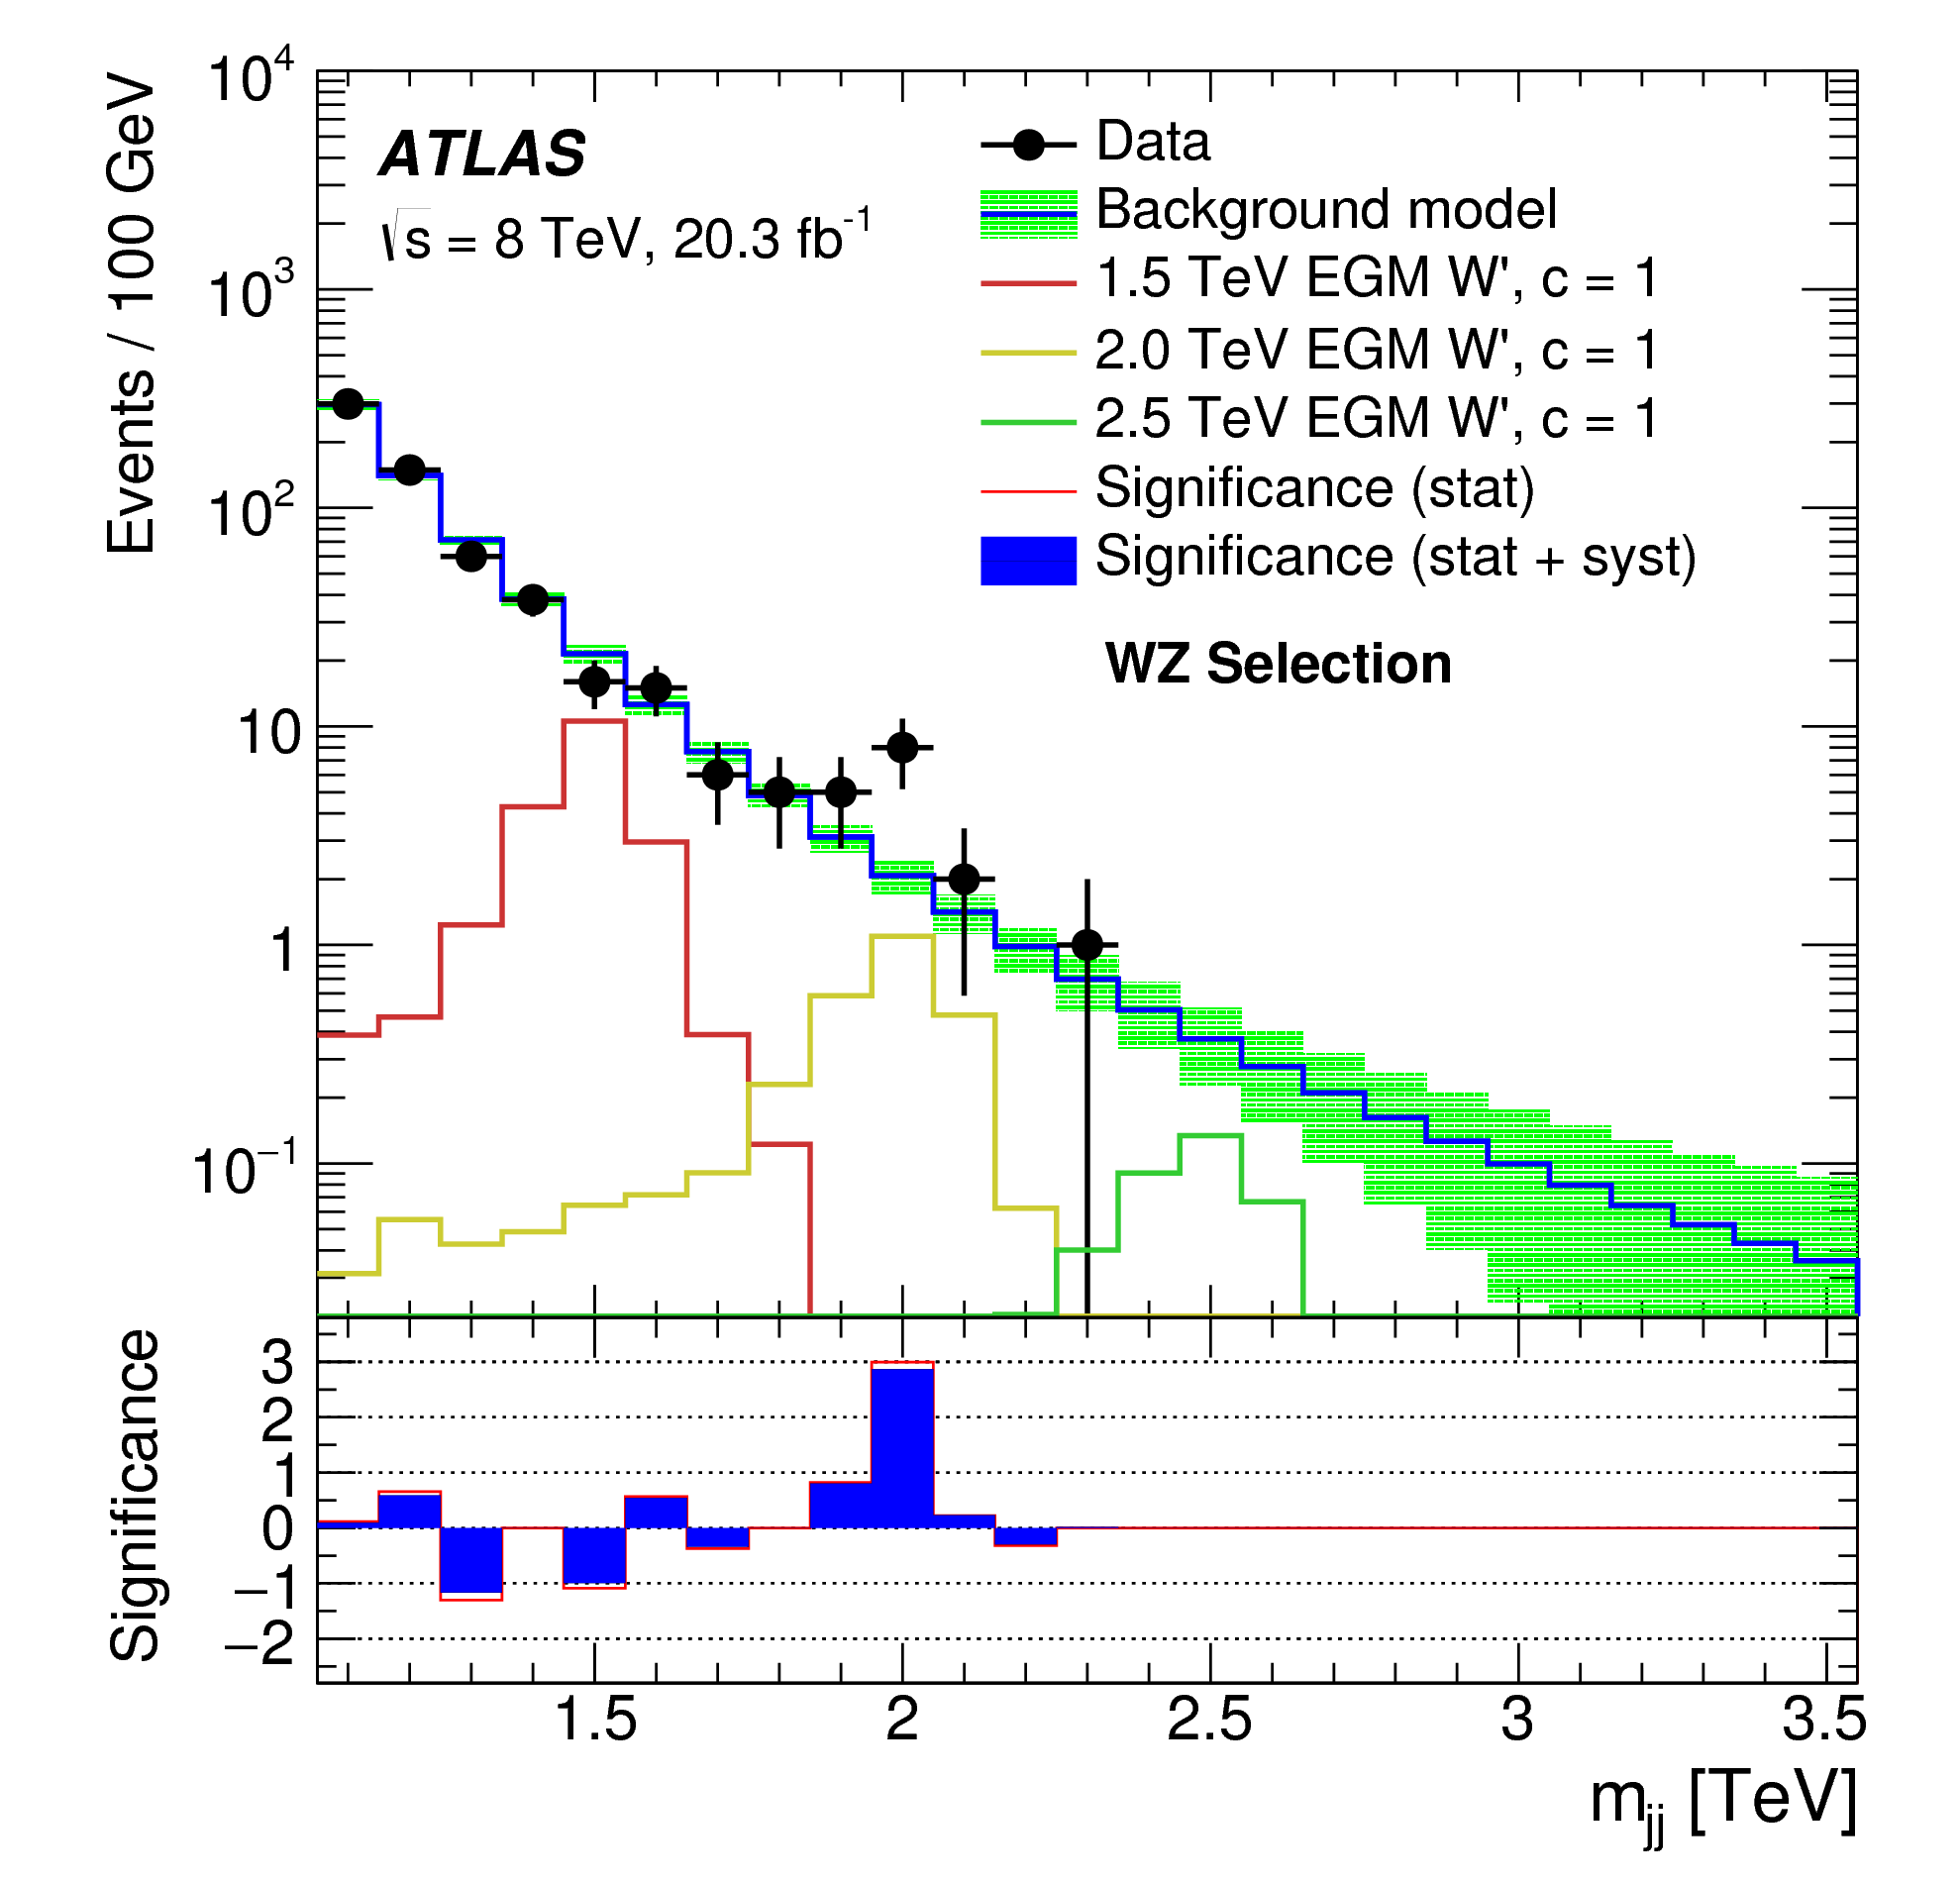
\includegraphics[width=0.4\textwidth]{figures/analysis/search1/misc/atlas_8tev.png}
    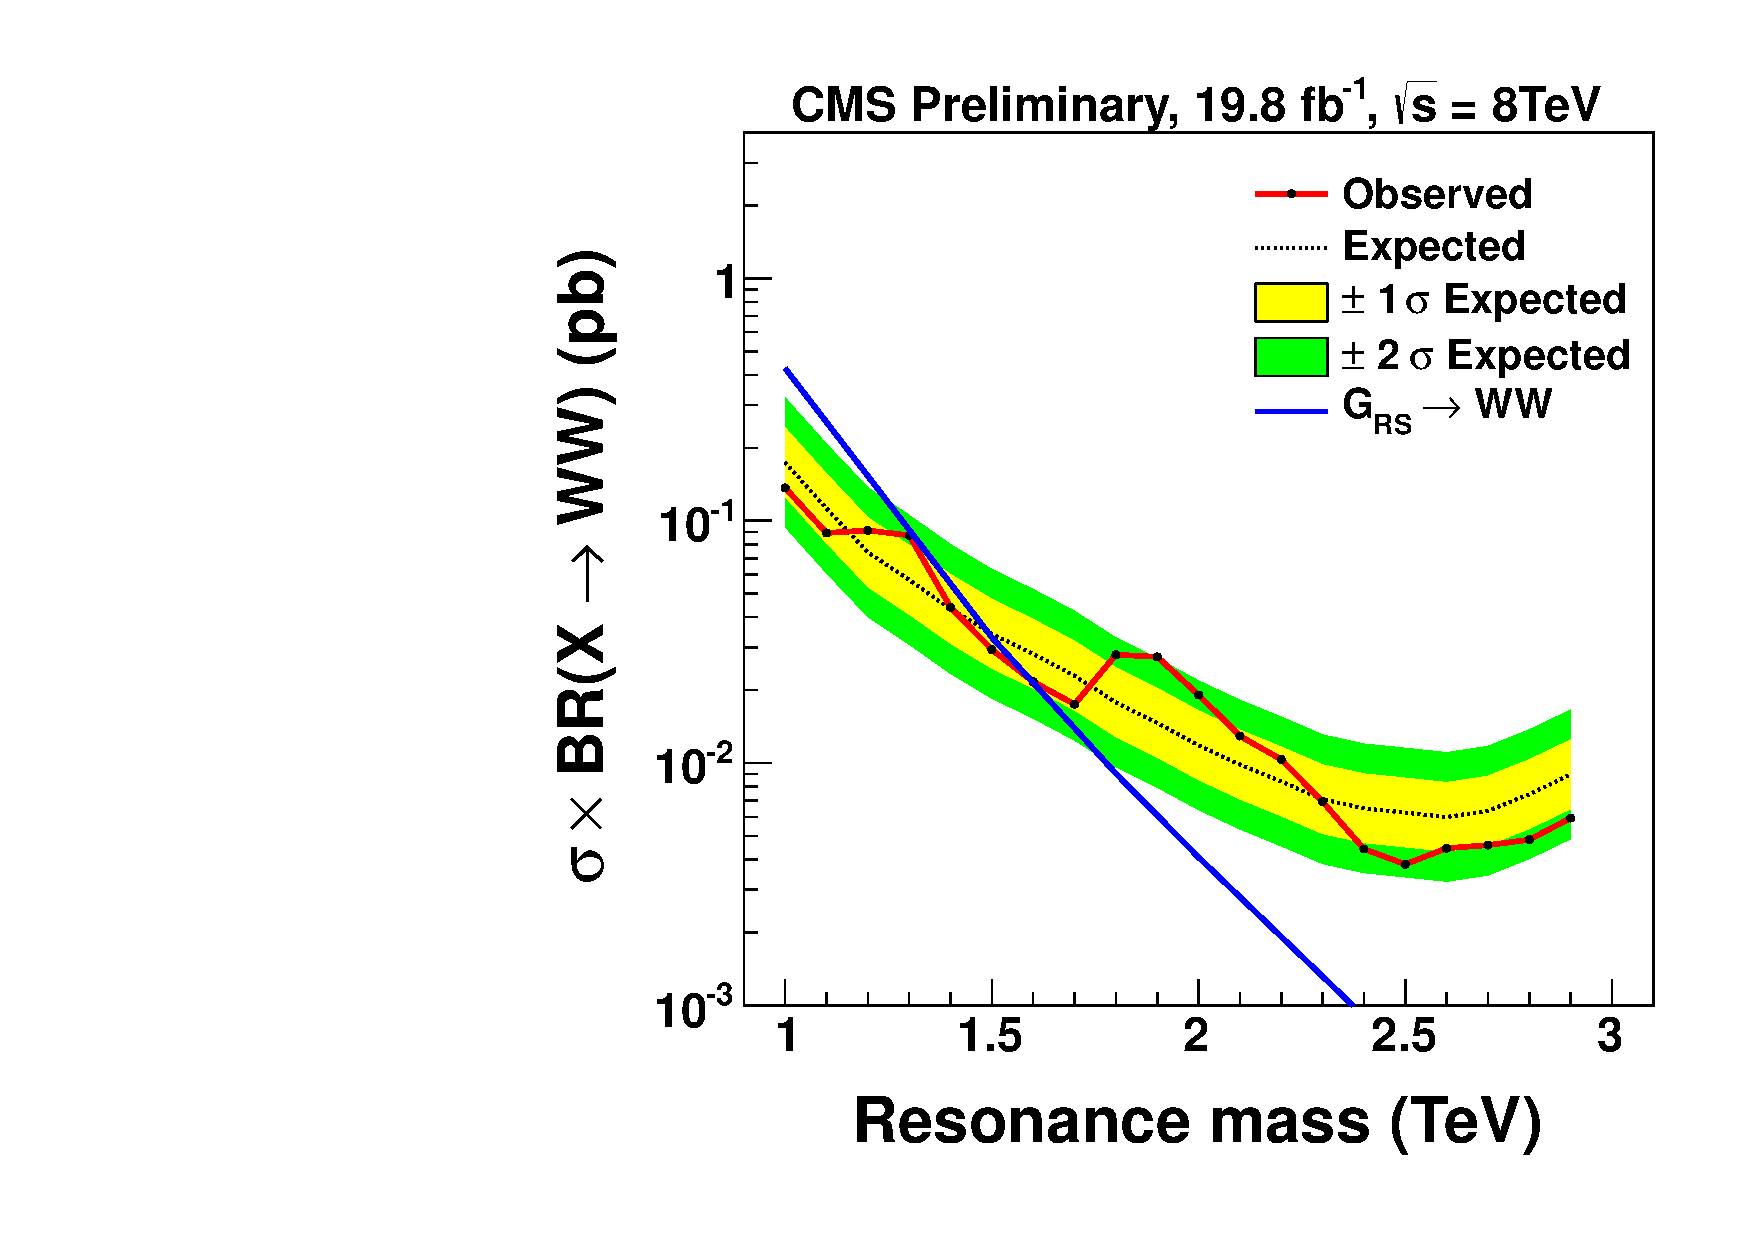
\includegraphics[width=0.4\textwidth]{figures/analysis/search1/misc/EXO-12-024_gWW.pdf}
    \caption{A "bump" corresponding to 3.4 $\sigma$ in the dijet invariant mass spectrum around 2 \TeV (left) observed by ATLAS when analyzing the full 8 \TeV dataset~\cite{Aad2015}, together with a similar excess (1.3 $\sigma$) observed in the corresponding CMS analysis~\cite{Khachatryan:1700394}.}
    \label{fig:searchI:8tev}
\end{figure}
The two measurements were found to be compatible, favoring a heavy resonance with a production cross section of around 5 femtobarn and a mass between 1.9 and 2.0 TeV decaying to either WW, WZ or ZZ~\cite{Dias:2015mhm}. Figure~\ref{fig:searchI:8tevcombo} shows the obtained p-value from the ATLAS (red) and CMS (blue) searches, as well as their combination (black). In addition to the observed excesses in the vector boson final states, another  $3 \sigma$ excess for a resonance with a mass of 1.8 \TeV had been observed in the search for heavy resonances decaying to a W and a Higgs boson~\cite{Khachatryan:2016yji} at 1.8 \TeV.
\begin{figure}[h!] 
    \centering
    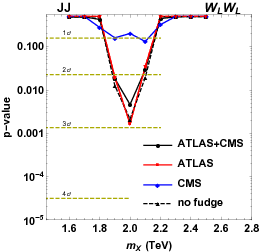
\includegraphics[width=0.25\textwidth]{figures/analysis/search1/misc/CMS_ATLAS_BulkWW_JJ_dijetfit_p.png}
    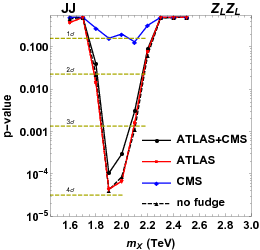
\includegraphics[width=0.25\textwidth]{figures/analysis/search1/misc/CMS_ATLAS_BulkZZ_JJ_dijetfit_p.png}
    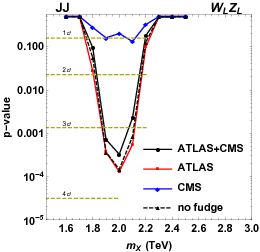
\includegraphics[width=0.25\textwidth]{figures/analysis/search1/misc/CMS_ATLAS_WZ_JJ_dijetfit_p.png}
    \caption{p-values as a function of resonance mass obtained with an emulation of the ATLAS (red) and CMS (blue) searches as well as the combination of the two (black). Here for a \PW\PW (left), \PW\PZ (middle) and \PZ\PZ (right) hypothesis~\cite{Dias:2015mhm}.}
    \label{fig:searchI:8tevcombo}
\end{figure}
The combination of the excesses and the timing of the ATLAS paper, naturally led to some excitement, and in the coming weeks, the arXiv was flooded with theory papers attempting an explanation of the deviations.\newline
In addition, one of the main benefits of increasing the LHC center-of-mass energy from 8 to 13 \TeV was that the partonic luminosity would increase.
One could therefore expect the same number of signal events in the 20 \fbinv data set collected with a center-of-mass energy of 8 TeV, for a considerably smaller luminosity with a center-of-mass energy of 13 TeV. Figure~\ref{fig:searchI:8vs13reach} shows the system mass that can be probed with the expected 2015 integrated luminosity of 3 \fbinv collected with a center-of-mass energy of 13 TeV, as a function of the probeable mass with 20 \fbinv of 8 TeV data for different partonic channels of qq, qg, and gg. For example, a 2 \TeV mass resonance would be observable in both datasets.
% The probable 13 \TeV mass is defined by finding the system mass which results in the same number of expected events at 8 \TeV, if assuming cross sections scale with partonic luminosity and $1/m^2$. Three different partonic scattering channels are considered: qq, qg and gg. We see that, for instance for a resonance with a mass of 2000 \GeV, the reach at 13 \TeV is 2241(gg), 2091(gq), 1851(qq, one type) and 2046(qq, all types) \GeV.
\begin{figure}[h!] 
    \centering
    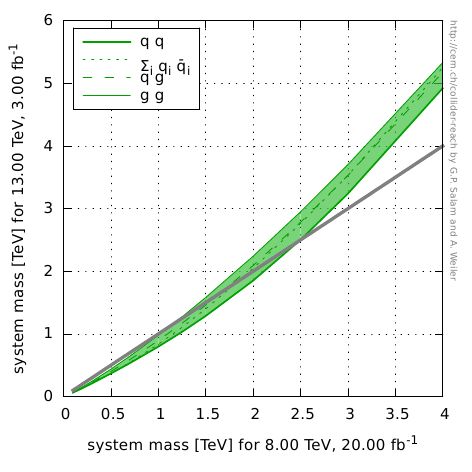
\includegraphics[width=0.50\textwidth]{figures/analysis/search1/misc/colliderReach.png}
    \caption{The system mass that can probed with 3 \fbinv of 13 \TeV data (y-axis) as a function of the probe-able system mass with 20 \fbinv of 8 \TeV data (x-axis) for different partonic channels (generated with~\cite{collreach}).}
    \label{fig:searchI:8vs13reach}
\end{figure}
We therefore expected that the small excess observed in the VV all-hadronic final state would be observable in the 2015 dataset if the signal was genuine.

\section{Analysis strategy}

When a resonance X with a mass above 1 TeV decays into a vector-boson pair, the bosons have a very high energy ($\tilde\PT=\mX/2=500 \GeV$, assuming X is produced at rest) is referred to as boosted. The decay products of a hadronically decaying boosted vector boson will therefore not appear as back-to-back in the lab frame but rather be collimated, as described in Section~\ref{sec:objreco:substructure}. This results in a final state with two high-pt, large-radius jets, such that the AK algorithm with an R=0.8 is expected to fully contain the two quarks coming from the vector boson decay. This is illustrated in Figure~\ref{fig:searchI:merged}.
\begin{figure}[h!] 
    \centering
    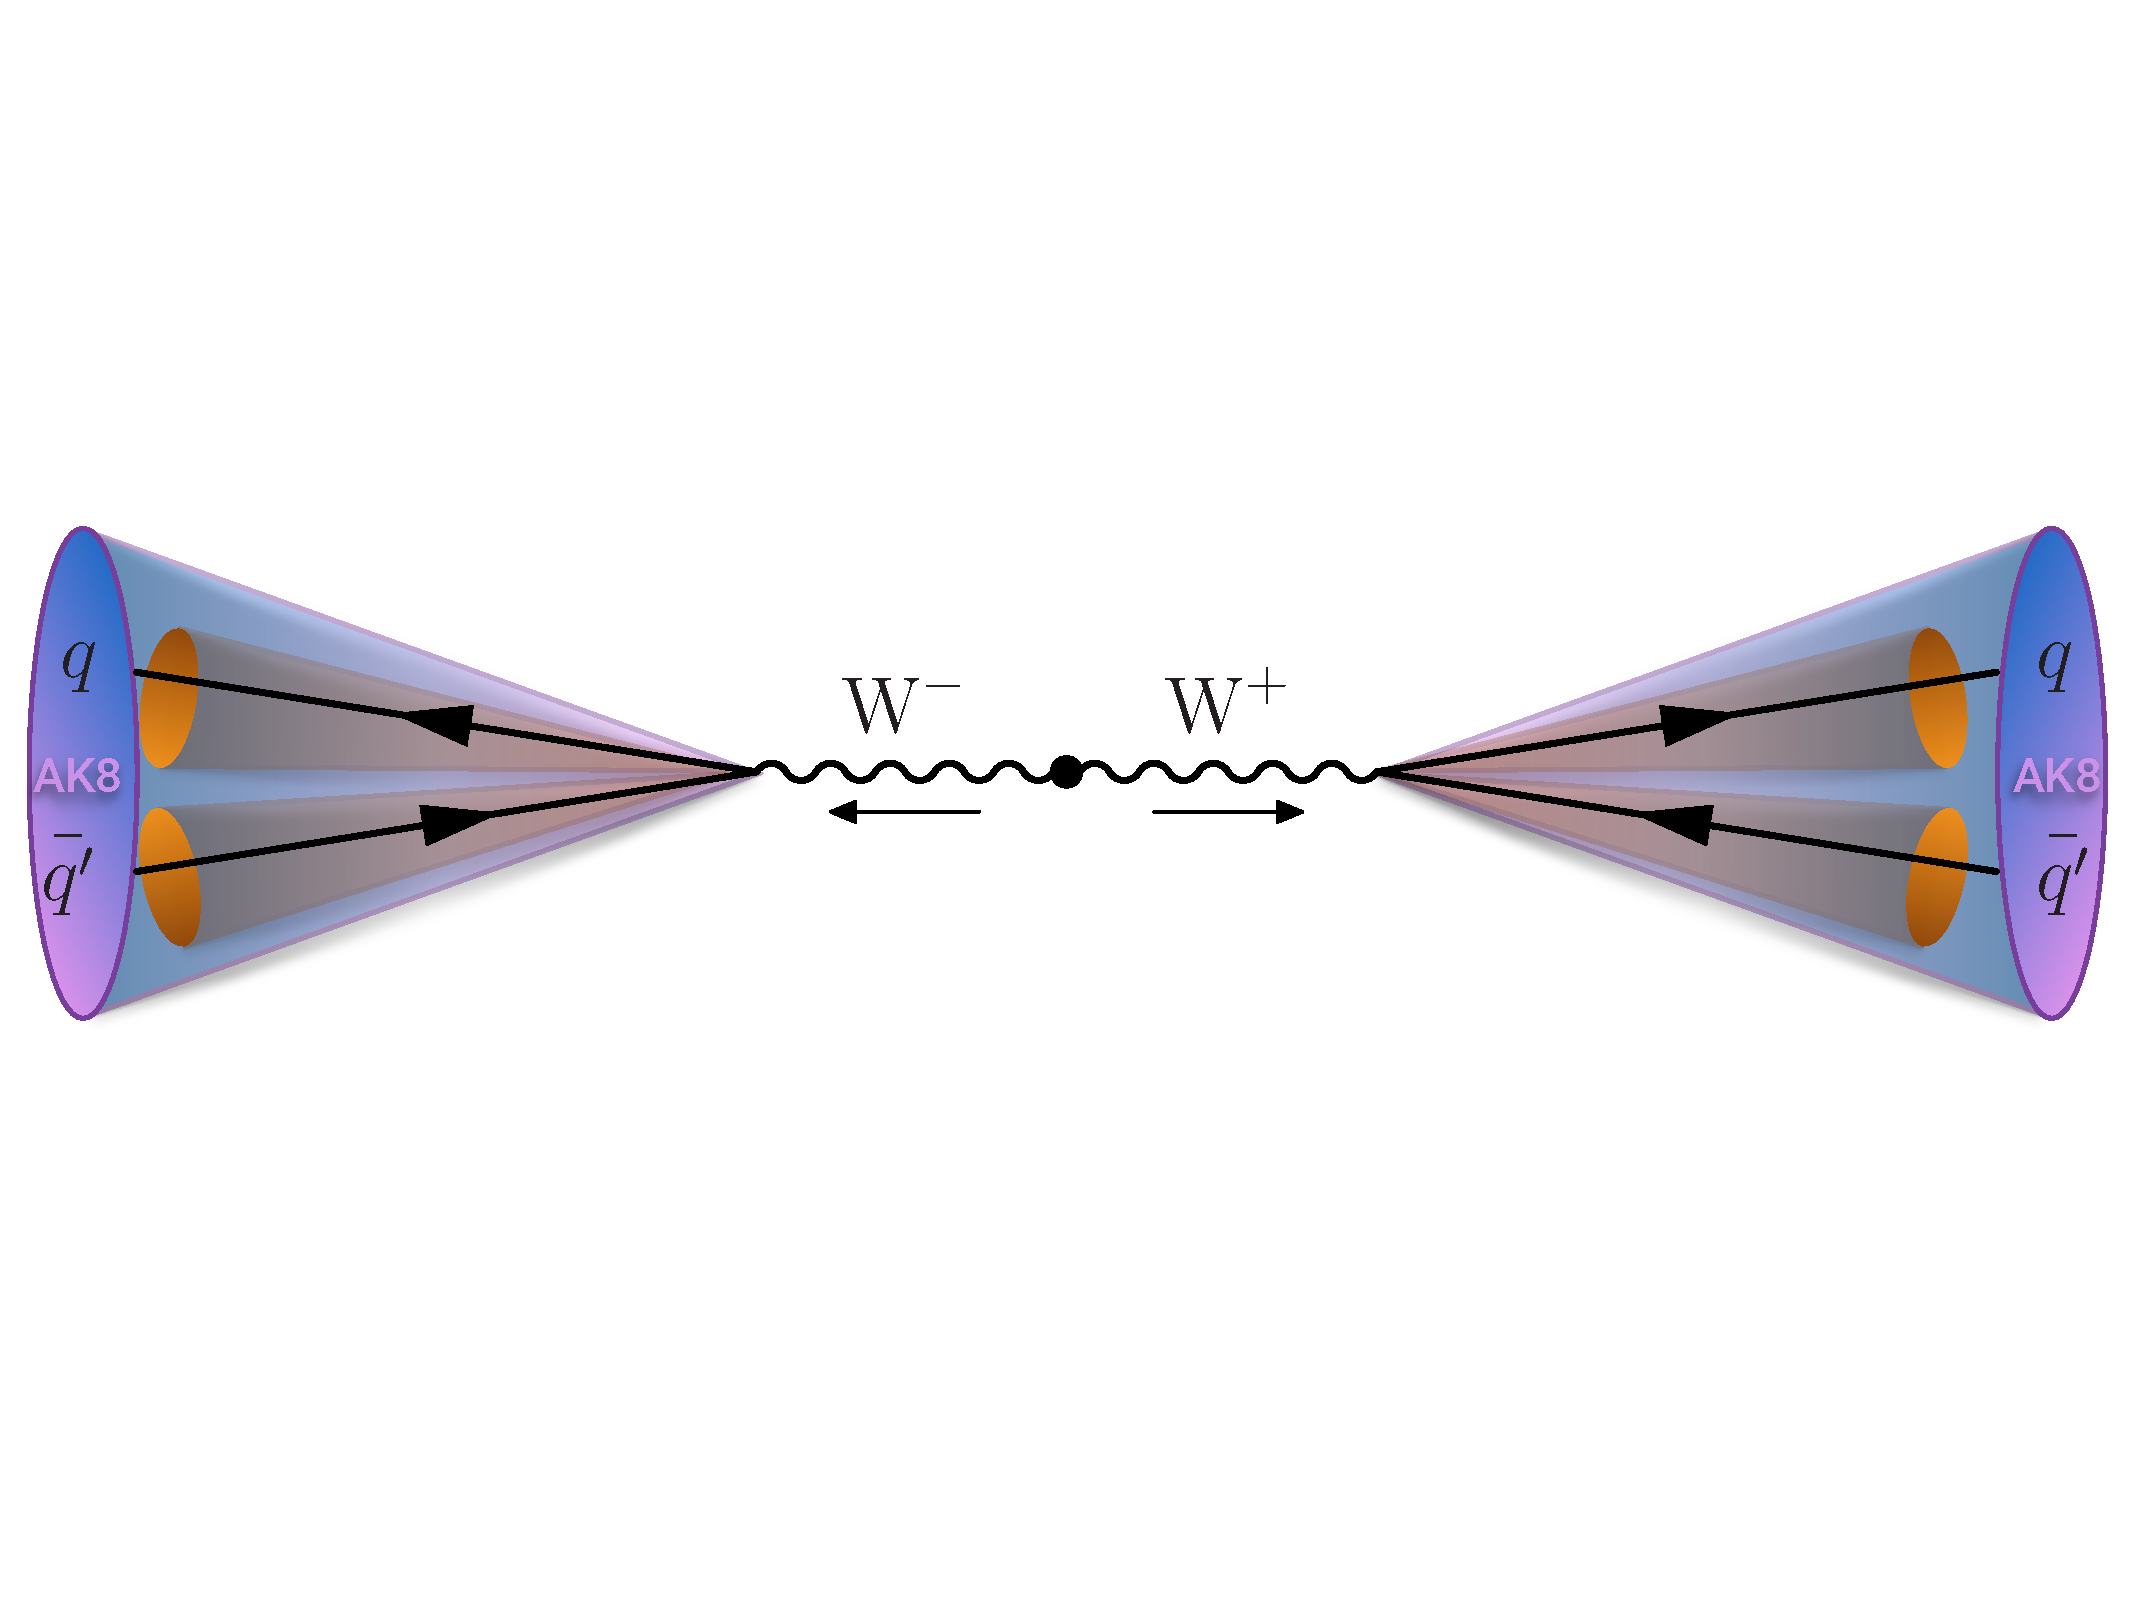
\includegraphics[width=0.70\textwidth]{figures/event_reconstruction/WWqqqq_merged_small.pdf}
    \caption{If a heavy ($>1 \TeV$) resonance decays into vector bosons, the transverse momentum of each boson will be large and its decay products are merged into one single large cone AK8 jet.}
    \label{fig:searchI:merged}
\end{figure}
The two jets are each expected to have a mass around the W or Z boson mass, and some intrinsic substructure stemming from their two-pronged decay. The invariant mass of the dijet system, \mjj, should be roughly equal to the resonance mass \mX. This dijet system is the final state under scrutiny and the dijet invariant mass is the parameter of interest. The final states of WW, ZZ, and WZ would produce similar final states. \par
The main background for such an analysis is QCD multijet events. As mentioned in Section~\ref{sec:objreco:substructure}, quark/gluon jets can obtain a high mass due to diffuse radiation and QCD processes have such a large cross section that the number of QCD jets with a mass compatible with the W mass can be large. In order to discriminate between the two, we take advantage of three properties. First, the groomed mass of signal and background jets should be very different. Second, signal jets should appear two-prong like, as opposed to quark/gluon jets, and third, the dijet invariant mass for the signal process should peak around the resonance mass while the QCD spectrum is predicted to be smoothly falling. Section~\ref{sec:searchI:bkg} explains this assumption in more detail. The strategy therefore consists of performing a smoothness test on \mjj of the observed data, a so-called "bump-hunt", by assuming that the signal will appear as a bump on top of a smooth distribution. This is illustrated in Figure~\ref{fig:searchI:bumphunt}.
\begin{figure}[h!] 
    \centering
    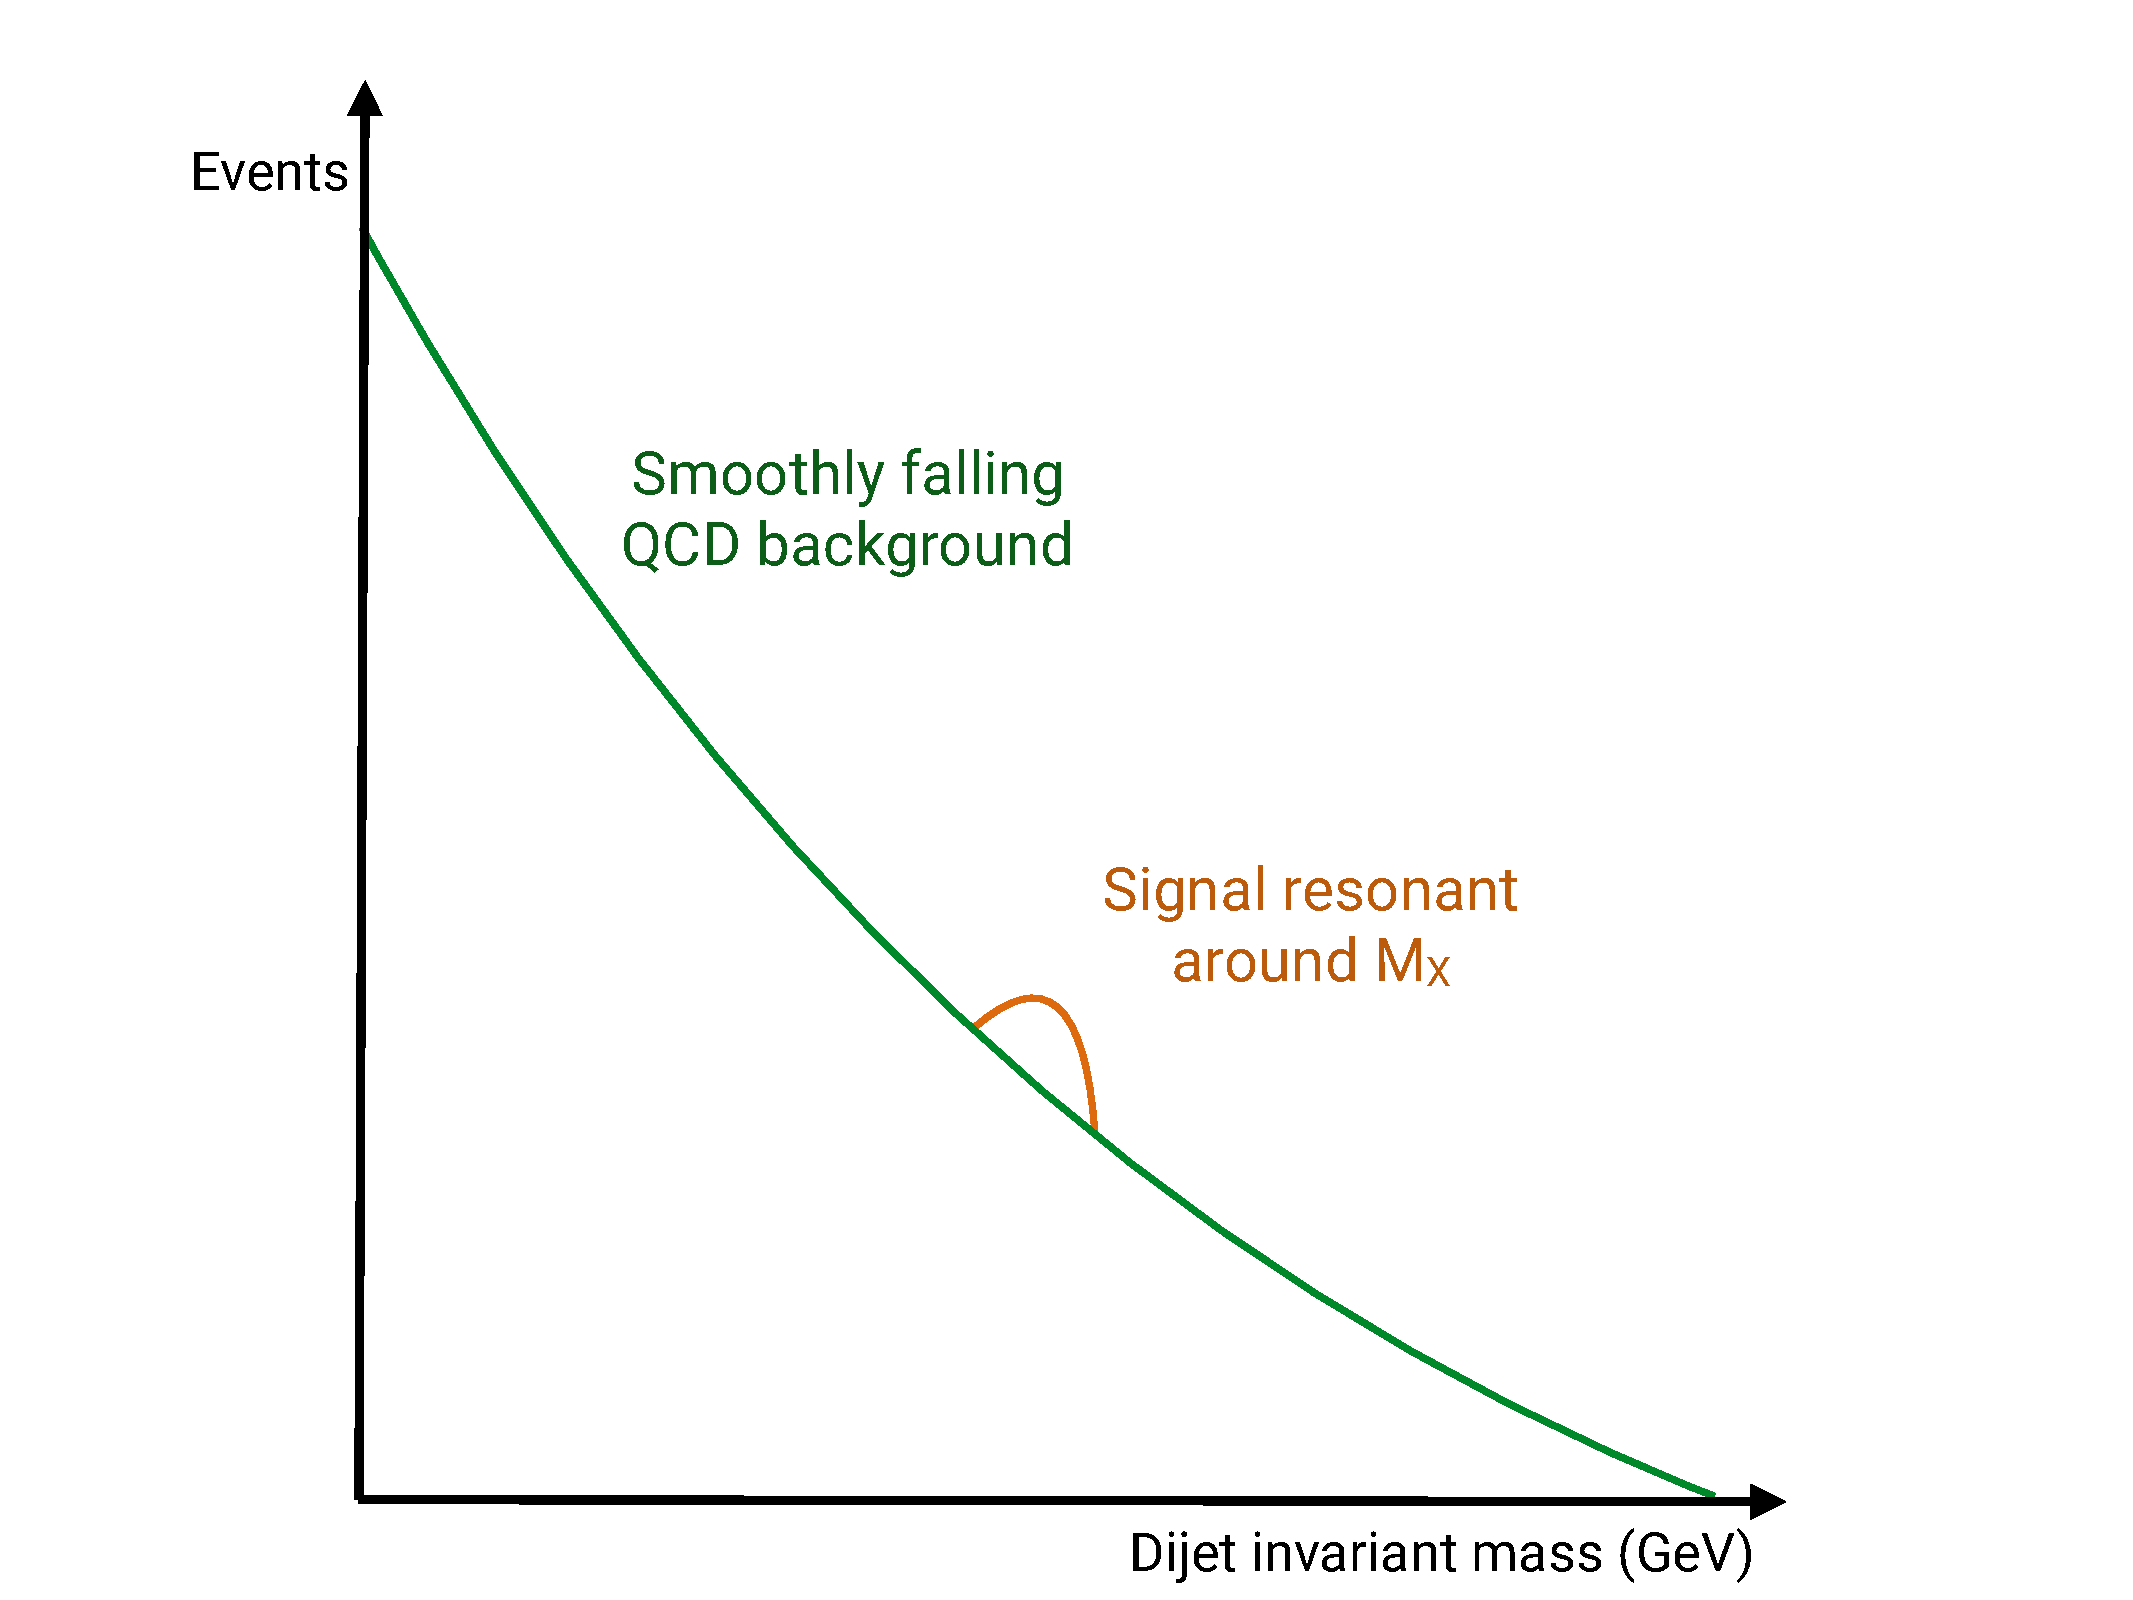
\includegraphics[width=0.49\textwidth]{figures/analysis/search1/misc/sigExtraction.pdf}
    \caption{The search strategy consists of looking for signal "bumps" in the dijet invariant mass on top of a smoothly falling QCD multijet background.}
    \label{fig:searchI:bumphunt}
\end{figure}
The benefit of such a method is that there is no need for a simulation of the background and the strategy is simple and robust. The disadvantage is that the analysis is intrinsically limited to regions where the dijet invariant mass spectrum is smooth and hence regions with discontinuities due to trigger turn-ons or kinematic selections must be avoided.

\section{Data and simulated samples}
\label{sec:searchI:samples}
The data analyzed in this search correspond to a total integrated luminosity of 2.7\fbinv collected at a center-of mass energy of 13 \TeV between June and December 2015. The instantaneous luminosity of the LHC during this run was around half of the design luminosity ($0.5 \times 10^{34} \percms$), with an average number of primary vertices per event of $<\mu>=13$. \par
The bulk graviton model (see Section~\ref{sec:theory:wed}) and the HVT model (\PWpr{} and \PZpr{}, see Section~\ref{sec:theory:hvt}) are used as benchmark signal processes. In these models, the vector gauge bosons are produced with a longitudinal polarization in more than 99\% of the cases, which leads to a 24\% higher acceptance per boson for reasons explained in Section~\ref{sec:objreco:pol}. For the HVT model, a scenario (model B) with $g_{\rm V}=3$, $c_{\rm H}=-0.976243$, and $c_{\rm F}=1.02433$ is chosen, where the heavy resonance predominantly couple to bosons and the coupling to fermions is suppressed. The bulk graviton samples were generated with $\ktilde = 0.5$. The resonance masses considered lie in the range 1.2 to 4 \TeV and are generated under the assumption of a natural width negligible with respect to the experimental resolution (narrow-width approximation). All signal samples are generated at leading order with \amcatnlo{} v2.2.2~\cite{Alwall:2014hca}. \par
Simulated samples of the production of QCD multijet events are generated to leading order using \PYTHIA version 8.205~\cite{Sjostrand:2007gs} with the CUETP8M1 tune~\cite{Khachatryan:2015pea} and are used to validate the analysis procedure.


\section{Event selection}

\subsection{Triggering}
\label{sec:searchI:trigger}
The first selection to be confronted in any analysis is the trigger selection. Due to an overwhelming QCD background in all-hadronic final states, the threshold for fully-hadronic triggers is very large in order to keep the trigger rate low (preferably around 10-30 Hz). In this analysis, we therefore decided to take advantage of triggers that place requirements on the jet's groomed mass in addition to the "standard" jet triggers based on the scalar sum of jet transverse energy \HT. These "boosted" triggers were never before tested in data, and this analysis was the first published result taking advantage of grooming at the trigger level in CMS. The following \HT-based High Level Triggers (HLT), referred to as inclusive triggers in the following, are used:
\begin{itemize}
  \itemsep0em 
\item {HLT\_PFHT650\_WideJetMJJ900DEtaJJ1p5},
\item {HLT\_PFHT650\_WideJetMJJ950DEtaJJ1p5}, and
\item {HLT\_PFHT800}.
\end{itemize}
Here, \emph{PFHT650} refers to a total \HT of at least 650 GeV. \emph{WideJet} means jets reconstructed with the \emph{wide jet algorithm}~\cite{2011123}, an algorithm inspired by jet grooming intended to reduce sensitivity to gluon radiation. The two AK R=0.4 jets with the largest \PT in the event are used as seeds. Geometrically close jets are then combined into the closest jet seed if they are within $\Delta R = \sqrt{(\Delta \eta)^2+\Delta \phi)^2}$, and these two jets form a dijet system used for further selections. \emph{MJJ900} refers to a wide-jet dijet mass of at least 900 GeV, and \emph{DetaJJ1p5} means there is an additional cut on the $|\Delta \eta|$ between the two wide jets for reasons that will be explained below. In addition, two triggers based on jet grooming are used. These require a trimmed jet mass (see Section 3.5.1) of 30 and 50 GeV, yielding the triggers:
\begin{itemize}
  \itemsep0em 
\item {HLT\_AK8PFJet360\_TrimMass30} and
\item {HLT\_AK8PFHT700\_TrimR0p1PT0p03Mass50}.
\end{itemize}
The tuneable parameters for the trimming algorithm are set to $r_{sub}=0.2$ and $p_{T,frac}=0.03$. The trigger requiring a trimmed jet mass of at least 30 GeV is seeded by single-object Level 1 triggers with jet $p_T$ thresholds of 176 or 200 GeV, and the remaining triggers require an online \HT of at least 150 or 175 GeV.\par
In order to avoid any kinks in the dijet invariant mass spectrum due to the presence of a trigger turn-on, we determine the dijet invariant mass at which the analysis triggers are fully efficient ($>99\%$), and only consider signal events above this value. In order to estimate the trigger efficiency, we use a trigger with a lower \HT threshold of 650 GeV as a reference trigger. This trigger has a prescale of 40, meaning events are only recorded one out of 40 times. It is seeded by L1 \HT triggers with thresholds of 150 or 175 GeV. We then define the efficiency as
\begin{equation*}
\textrm{Efficiency} = \frac{N_{trigger+ref}}{N_{ref}}  
\end{equation*}
where $N_{trigger+ref}$ corresponds to the number of events passing the trigger under study as well as the reference trigger, and $N_{ref}$ corresponds to the number of events passing the reference trigger. Figure~\ref{fig:searchI:trigger-fits} shows the trigger turn-on curves as a function of dijet invariant mass for jets where one of the jets is required to have a pruned mass larger than 65 GeV (in other words, compatible with a W jet). A sharp turn-on for the inclusive triggers (top left) is observed, reaching the 100\% efficiency plateau for dijet masses of around 1.0--1.1 TeV. The grooming triggers, however, turn on more slowly and are not fully efficient until dijet invariant masses reach around 1.2 TeV (top right). The real power of the grooming triggers become clear when considering them in addition to the \HT-based triggers. The bottom plot in Figure~\ref{fig:searchI:trigger-fits} compares the trigger turn-on curves as a function of dijet invariant mass for jets passing one of the three inclusive triggers only, one of the grooming triggers only, and when combining all of them. Here, one can see that the 99\% efficiency threshold is lowered by 75 \GeV when including the substructure triggers, once substructure is required at analysis level. This combination of triggers allowed the analysis to consider dijet invariant masses as low as 1 TeV.
\begin{figure}[h!]
\centering
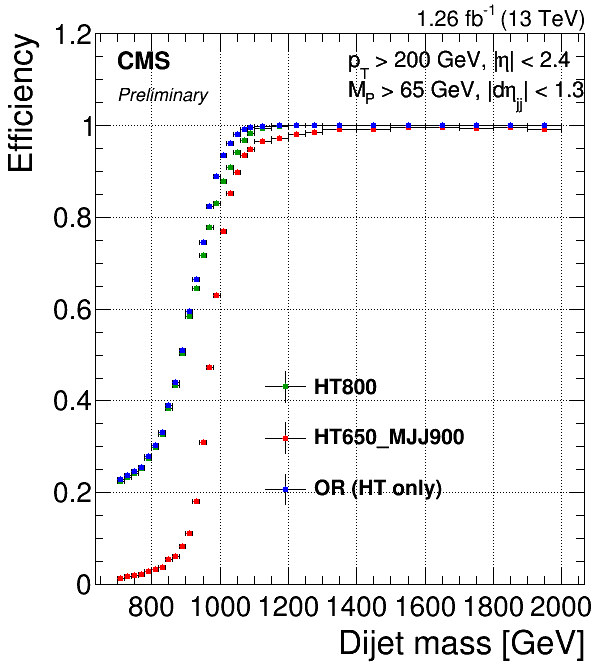
\includegraphics[width=0.4\textwidth]{figures/analysis/search1/AN-15-211//triggereffMjj-HT.png}
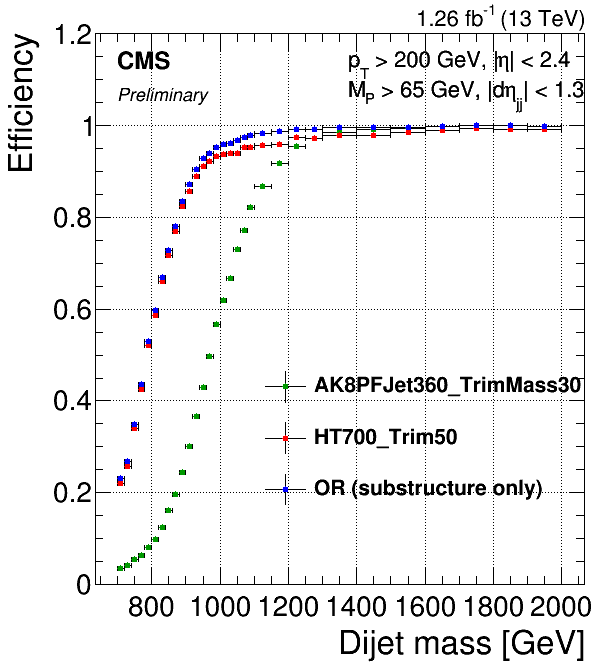
\includegraphics[width=0.4\textwidth]{figures/analysis/search1/AN-15-211//triggereffMjj-SUBST.png}\\
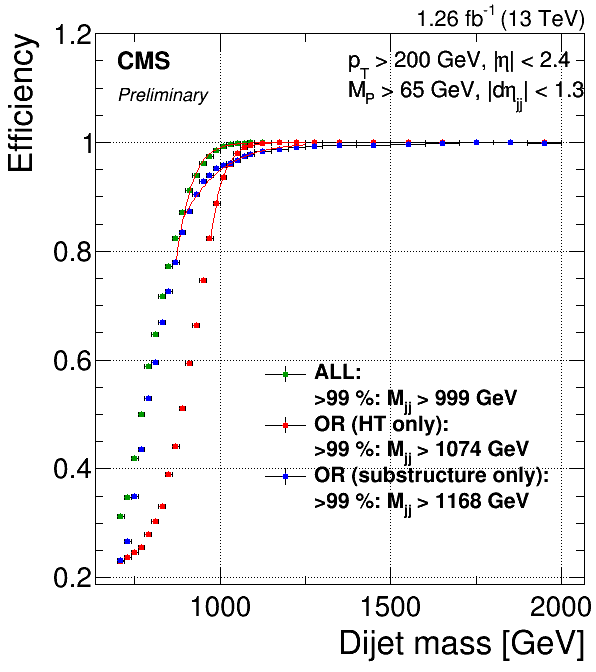
\includegraphics[width=0.4\textwidth]{figures/analysis/search1/AN-15-211/triggereffMjj-ALL.png}
\caption{Top: Efficiency for the inclusive triggers (top left) and the grooming triggers (top right) as a function of dijet invariant mass for jet pairs where one jet has a pruned mass larger than 65 GeV. Bottom: Comparison of trigger efficiencies for jets passing one of the HT-triggers only (red), for jets passing one of the grooming-triggers only (blue) and for jets passing one of the HT-triggers or one of the grooming triggers (green). Here as a function of dijet invariant mass for all jet pairs passing loose selections and where one jet has a pruned mass larger than 65 GeV. The 99\% efficiency threshold is lowered by 75 \GeV when including substructure taggers.}
\label{fig:searchI:trigger-fits}
\end{figure}
As a measure of the performance of the grooming triggers, we have in addition looked at the trigger efficiencies as a function of the offline groomed mass (using the pruned and softdrop algorithms described in Sections~\ref{sec:objreco:pruning} and ~\ref{sec:objreco:softdrop}), for the grooming trigger with the lowest mass threshold (30 \GeV). This is shown in Figure~\ref{fig:searchI:grooming-mj-trigger}, where an additional cut on the jet transverse momentum of one of the jets of 600 GeV is required and no other mass cut is applied. The trigger plateau is reached for offline groomed-jet masses around 50 GeV. 
\begin{figure}[h!]
\centering
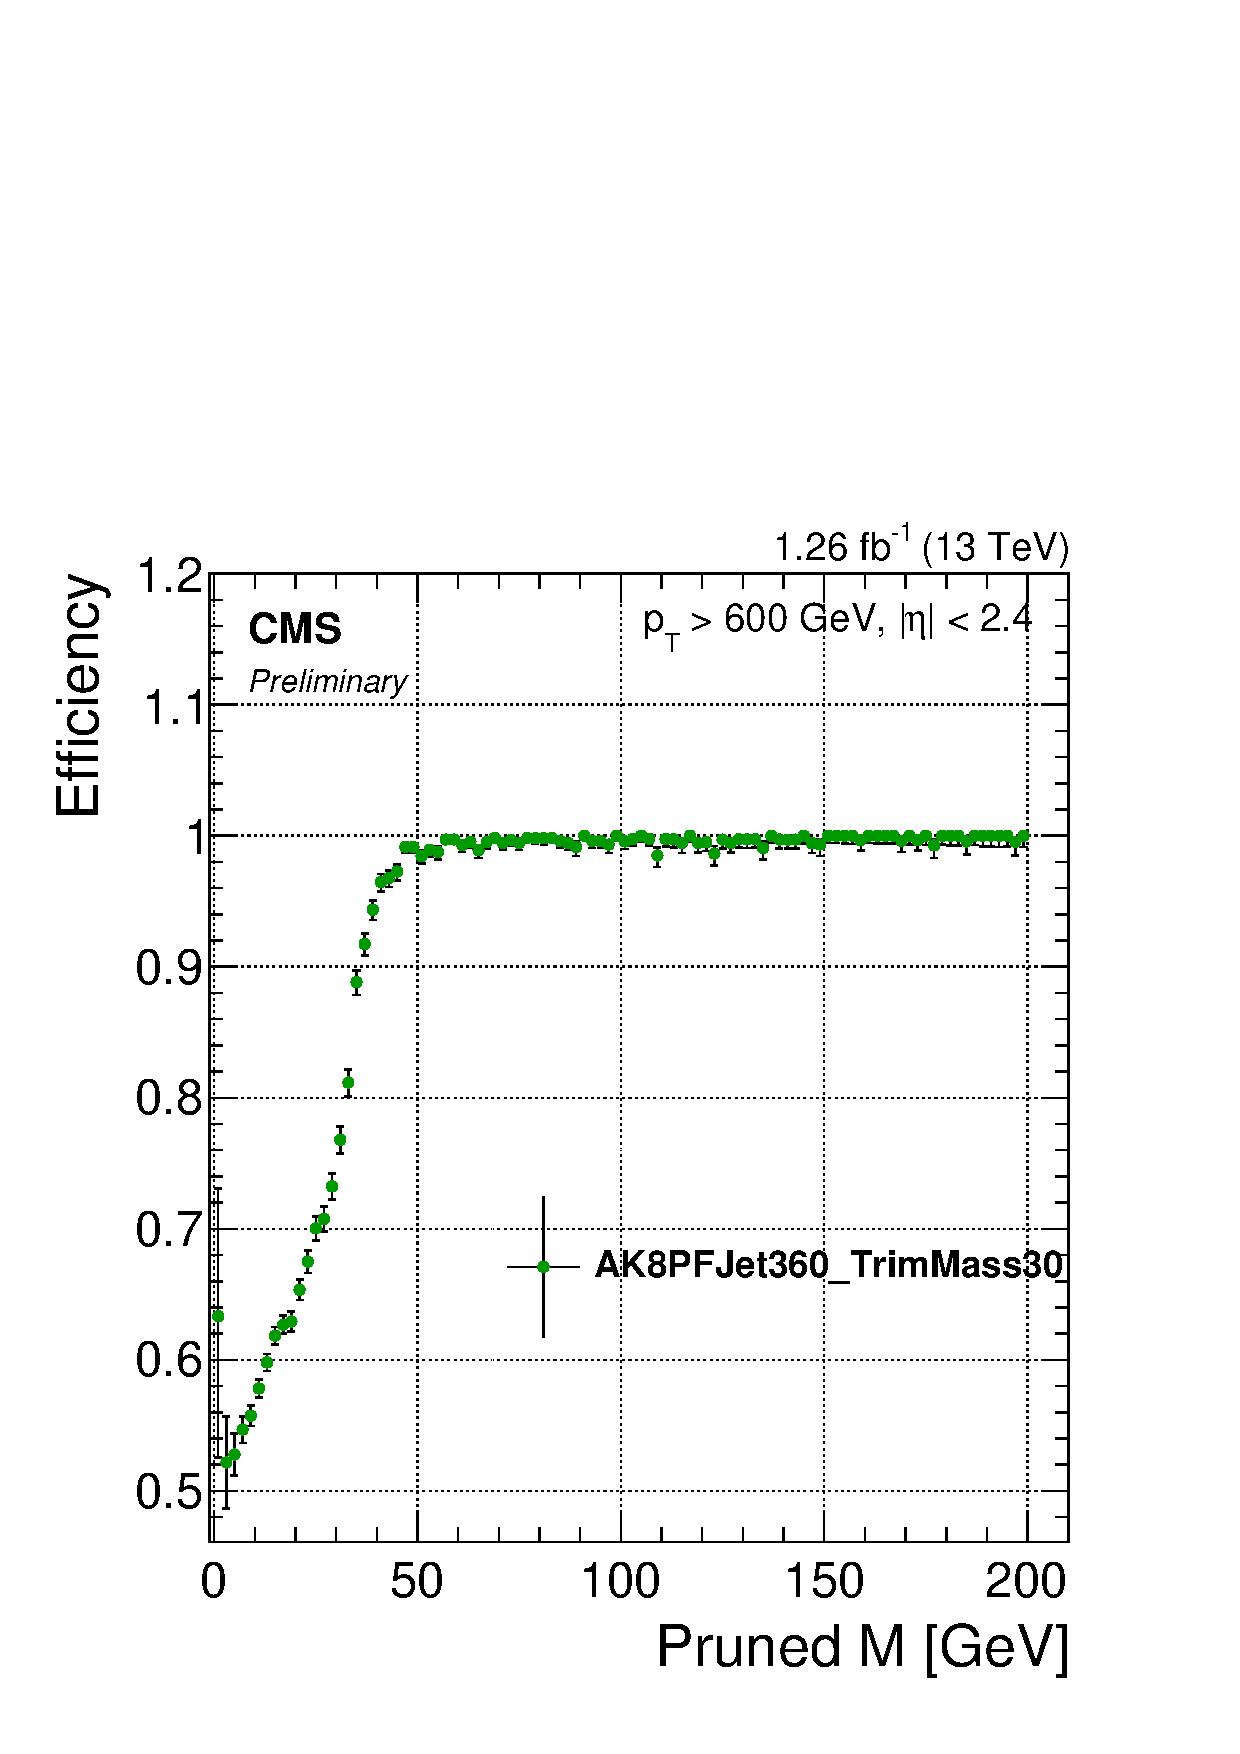
\includegraphics[width=0.4\textwidth]{figures/analysis/search1/AN-15-211//triggereff-prunedmass600.pdf}
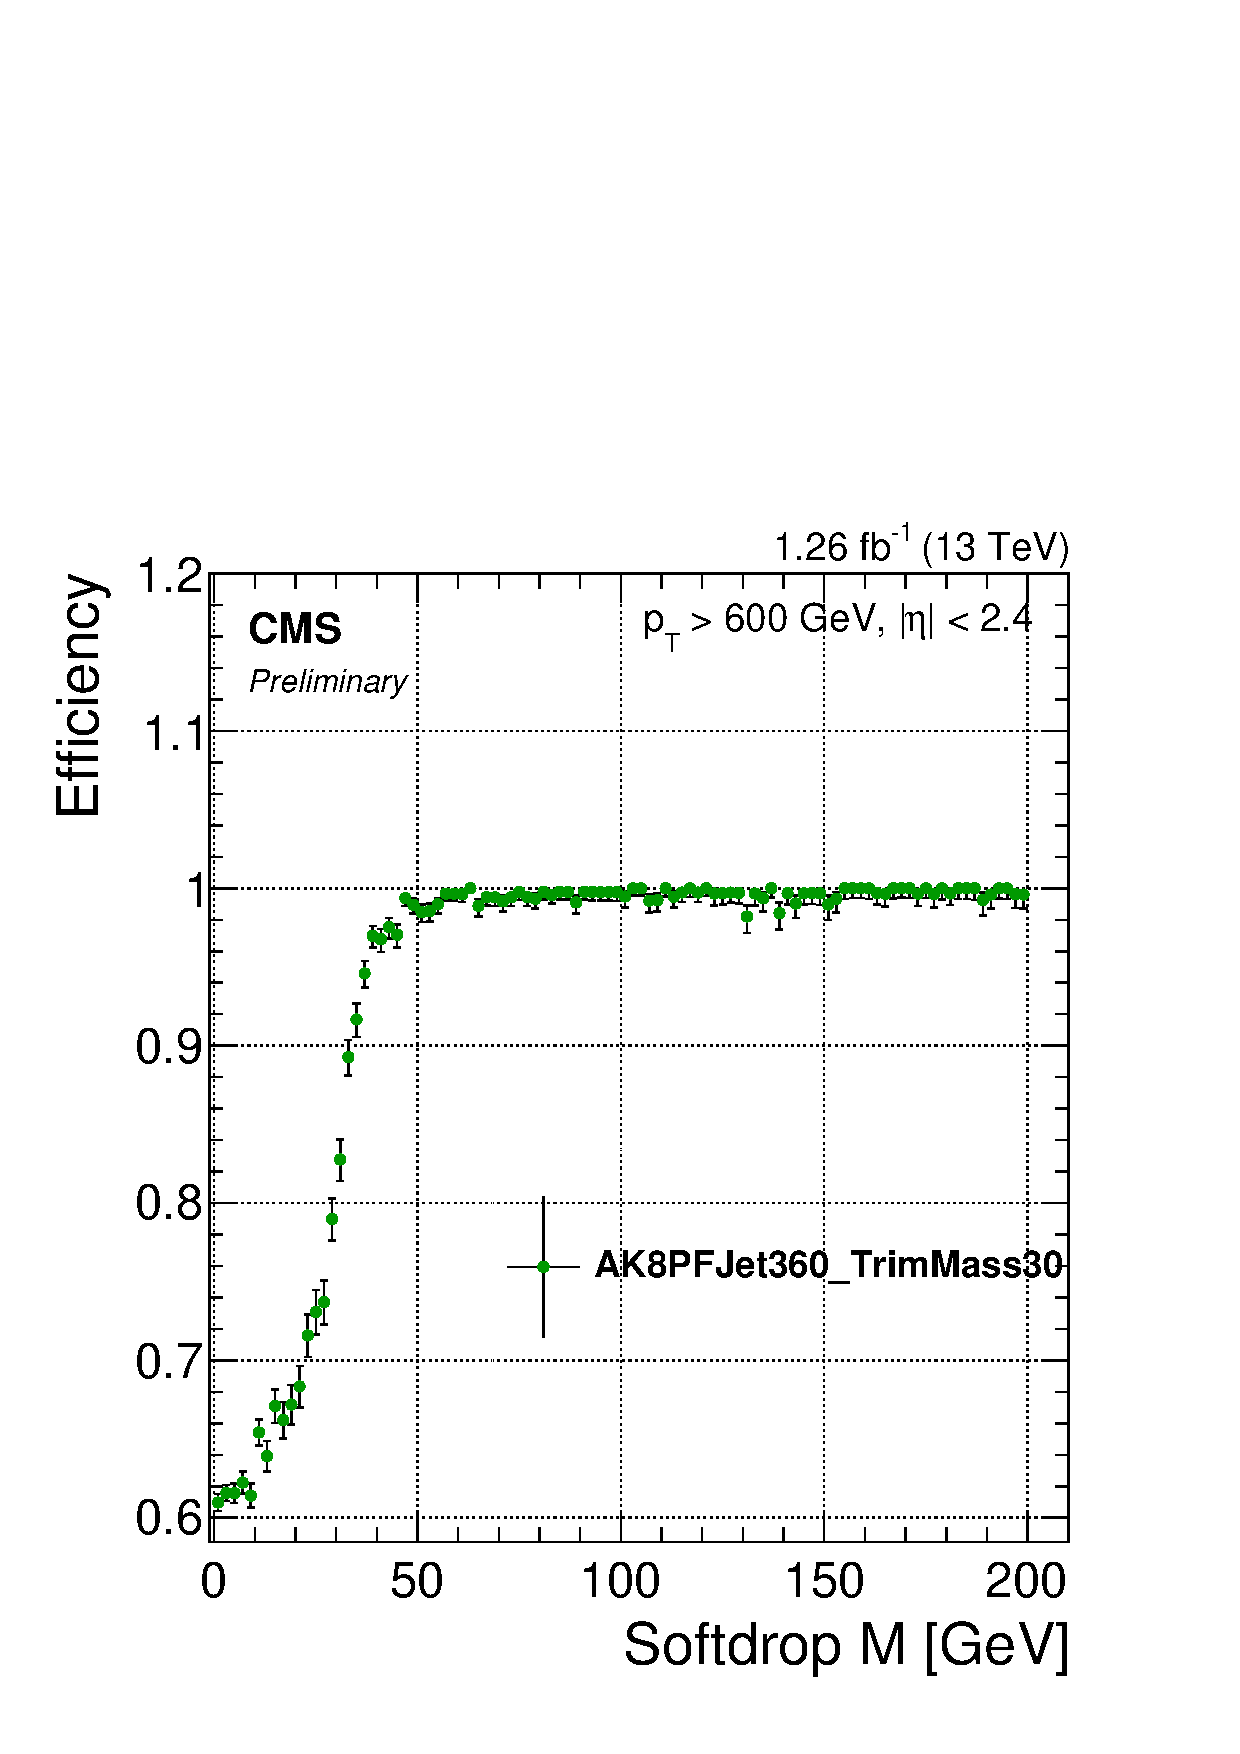
\includegraphics[width=0.4\textwidth]{figures/analysis/search1/AN-15-211//triggereff-sdmass.pdf}
\caption{Efficiency for the lowest threshold grooming trigger as a function of pruned-jet (left) and softdrop-jet (right) mass for jets with $\PT > \unit{600}{\GeV}$.}
\label{fig:searchI:grooming-mj-trigger}
\end{figure}

\subsection{Preselection} 
\label{sec:searchI:preselection}
After trigger selections, and the corresponding requirement of a dijet invariant mass above 1 \TeV to ensure a smoothy falling background, we begin the process of maximizing the signal significance while keeping the background low. This is done by optimizing the selection requirements on the jets. The jets used in this analysis are clustered with the anti-\kt{} jet clustering algorithm with a clustering parameter of $R=0.8$ (see Section ~\ref{sec:objreco:jets}) to allow containment of the full vector-boson decay products. Since a minimum transverse momentum of 200 \GeV is required for the decay products of a W/Z to be fully contained within an R=0.8 jet, events are further selected by requiring at least two jets with $\PT > \unit{200}{\GeV}$. These are in addition required to be central, with an $|\eta| < 2.4$. The two highest \PT jets in the event passing these criteria are selected as potential vector boson candidates. As our main background is QCD multijet events, we further take advantage of the fact that the angular distribution between these, mainly t-channel, processes are very different from the s-channel signal processes under study. The crossection for QCD t-channel processes as a function of the opening angle with respect to the beam axis ($\theta*$), exhibit a pole around $\cos \theta*=1$, meaning QCD t-channel jets are mostly produced in the forward direction, with an opening angle with respect to the beam axis close to zero. The signal jets on the other hand, produced through an s-channel process, are concentrated in the barrel region. We therefore require the jets to have a separation of $|\Delta\eta|<1.3$ in order to reduce the QCD multijets background. The distribution of $|\Delta\eta|$ between the two highest-\PT jets for QCD, as well as for different signal scenarios, is shown in Figure~\ref{fig:searchI:detaopt}.
\begin{figure}[h!]
\centering
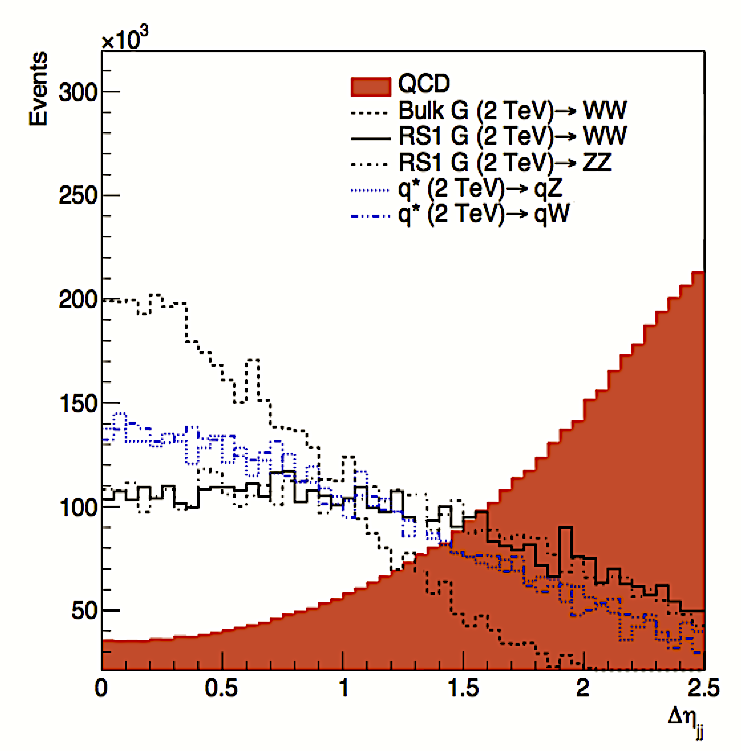
\includegraphics[width=0.4\textwidth]{figures/analysis/search1/misc/deta_opt.png}
\caption{ $|\Delta\eta|$  between the two highest-\PT jets for QCD jets and jets stemming from different signal scenarios.}
\label{fig:searchI:detaopt}
\end{figure}
A cut of $|\Delta \eta|_{jj}<1.3$ removes the t-channel pole at $\cos \theta* = 1$ and is in addition found to yield the highest signal sensitivity. In addition to these requirements on the jets themselves, a veto on jets overlapping with leptons is applied. Here the overlap $\Delta R(\text{jet},\text{lepton})$ between the jet candidate and a lepton is required to be larger than 0.8. Leptons used for this veto are required to pass the identification requirements described in Section~\ref{sec:objreco:electrons} and~\ref{sec:objreco:muons}, have a transverse momentum larger than 35 (30) GeV, and a pseudorapidity smaller than 2.5 (2.4) in the case of electrons (muons). The \PT, $\eta$, dijet invariant mass, and $|\Delta \eta|_{jj}$ distribution for the two leading jets in the event after the above preselections have been applied is shown in Figure~\ref{fig:kinematics-all}.
\begin{figure}[h!]
\centering
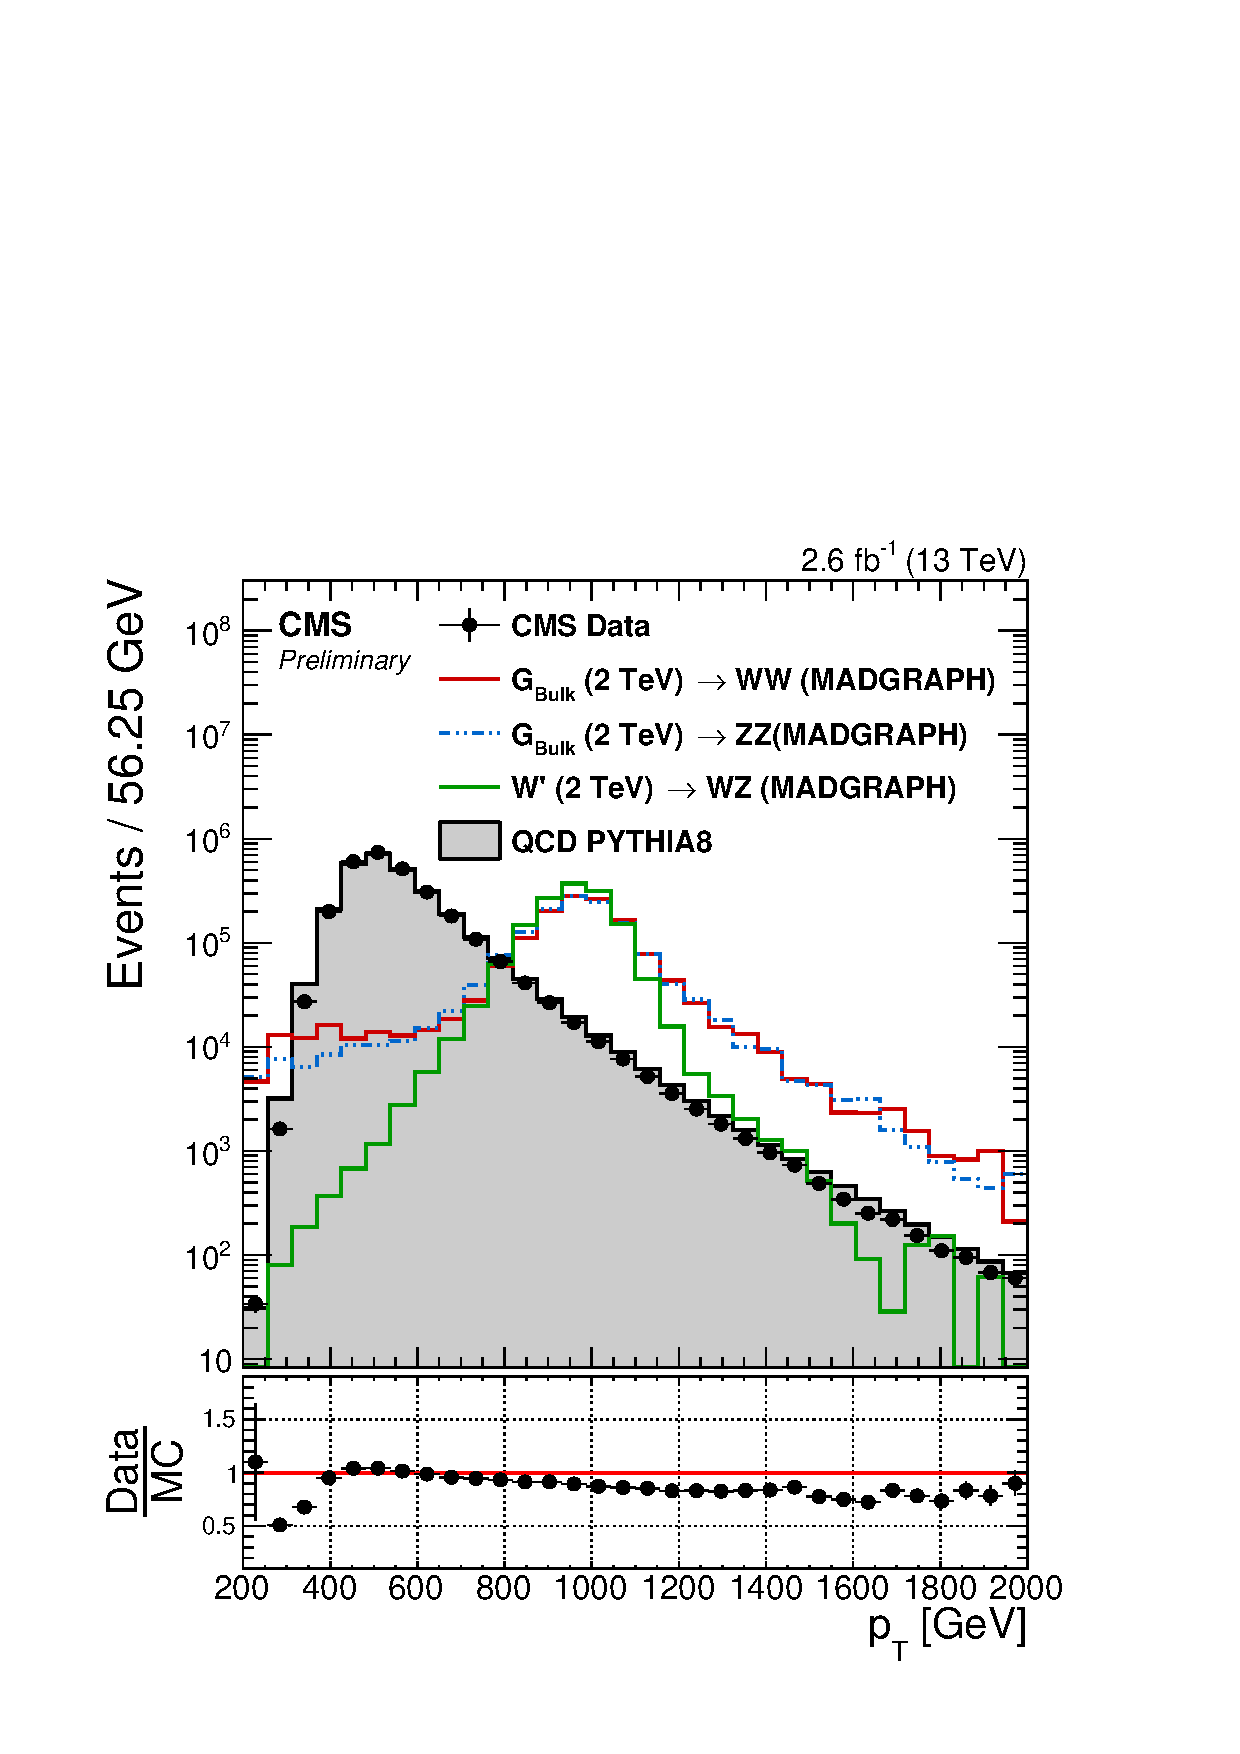
\includegraphics[width=0.4\textwidth]{figures/analysis/search1/AN-15-211/controlplots/silverjson/Pt_WSignal.pdf}
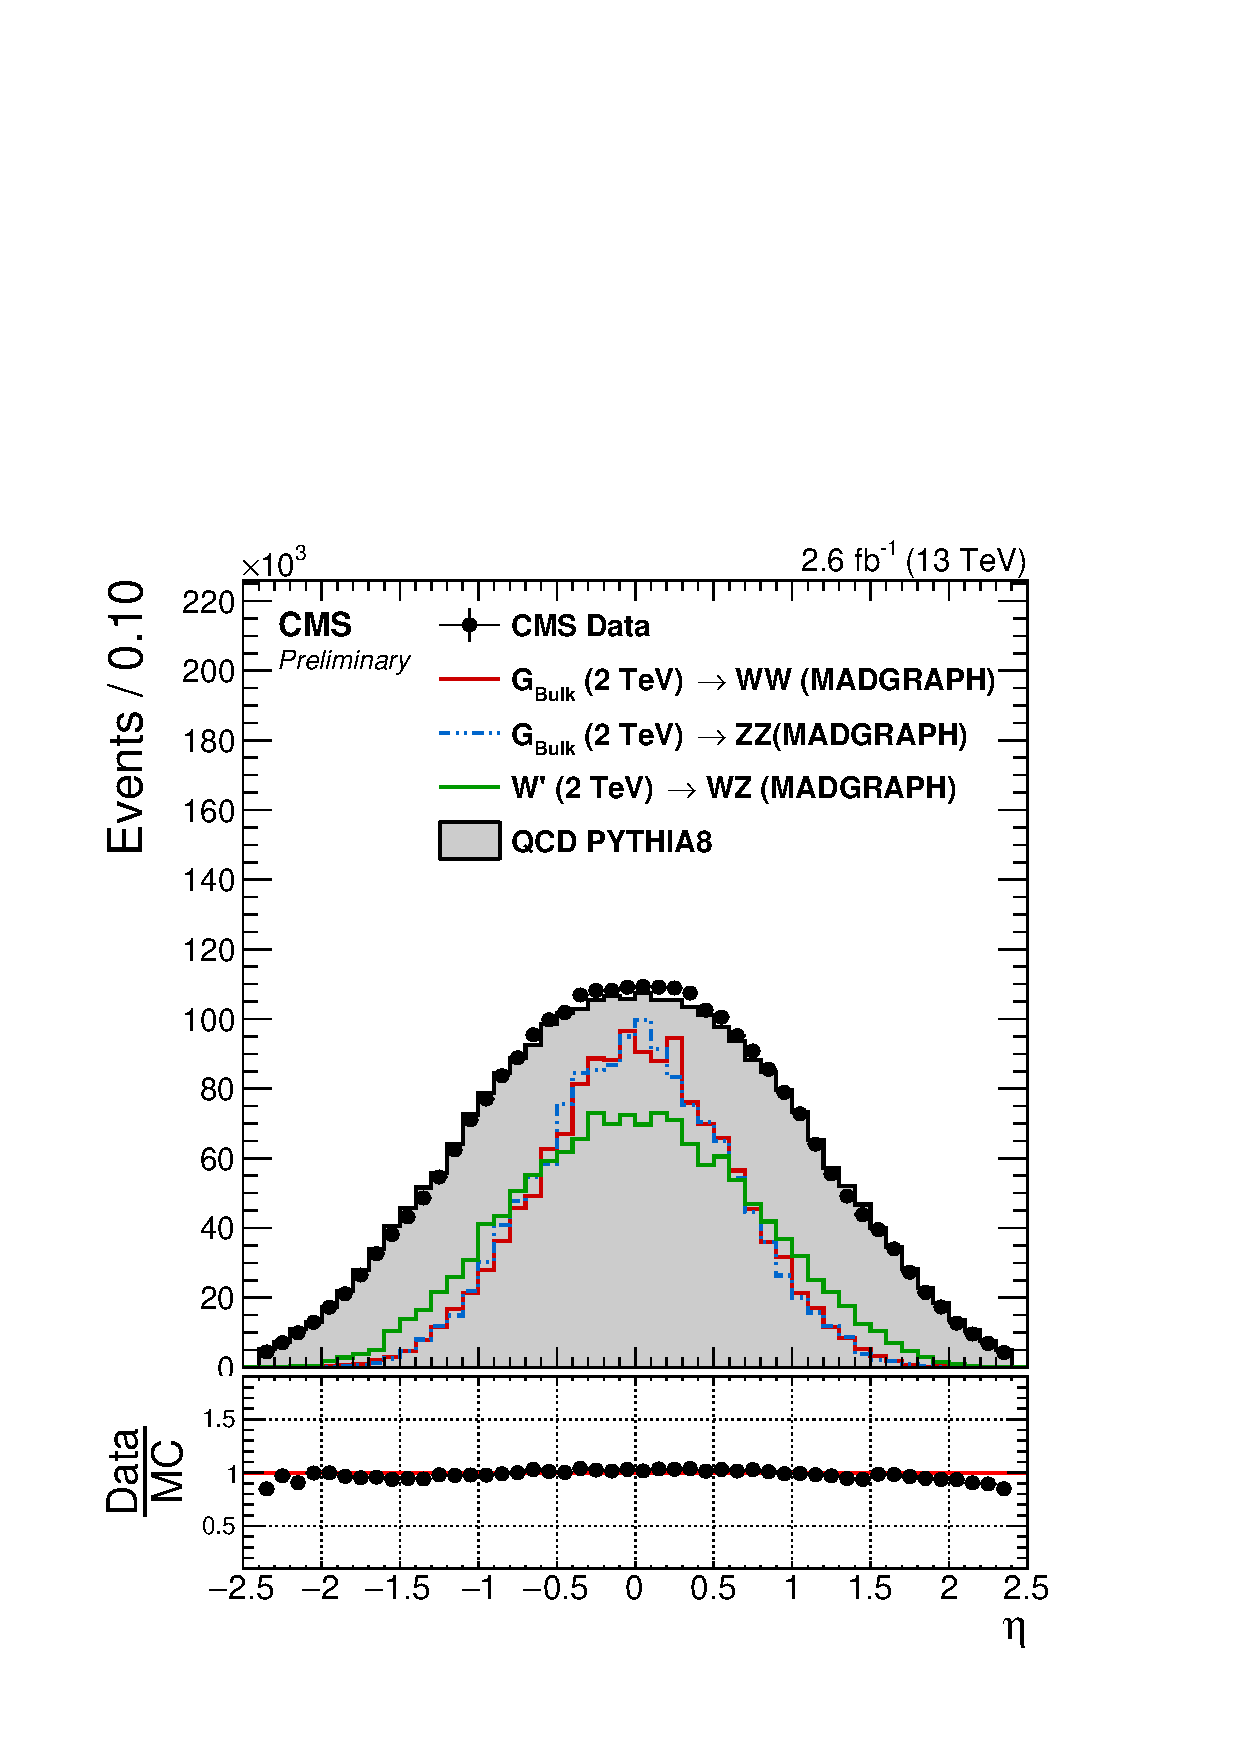
\includegraphics[width=0.4\textwidth]{figures/analysis/search1/AN-15-211/controlplots/silverjson/Eta_WSignal.pdf}\\
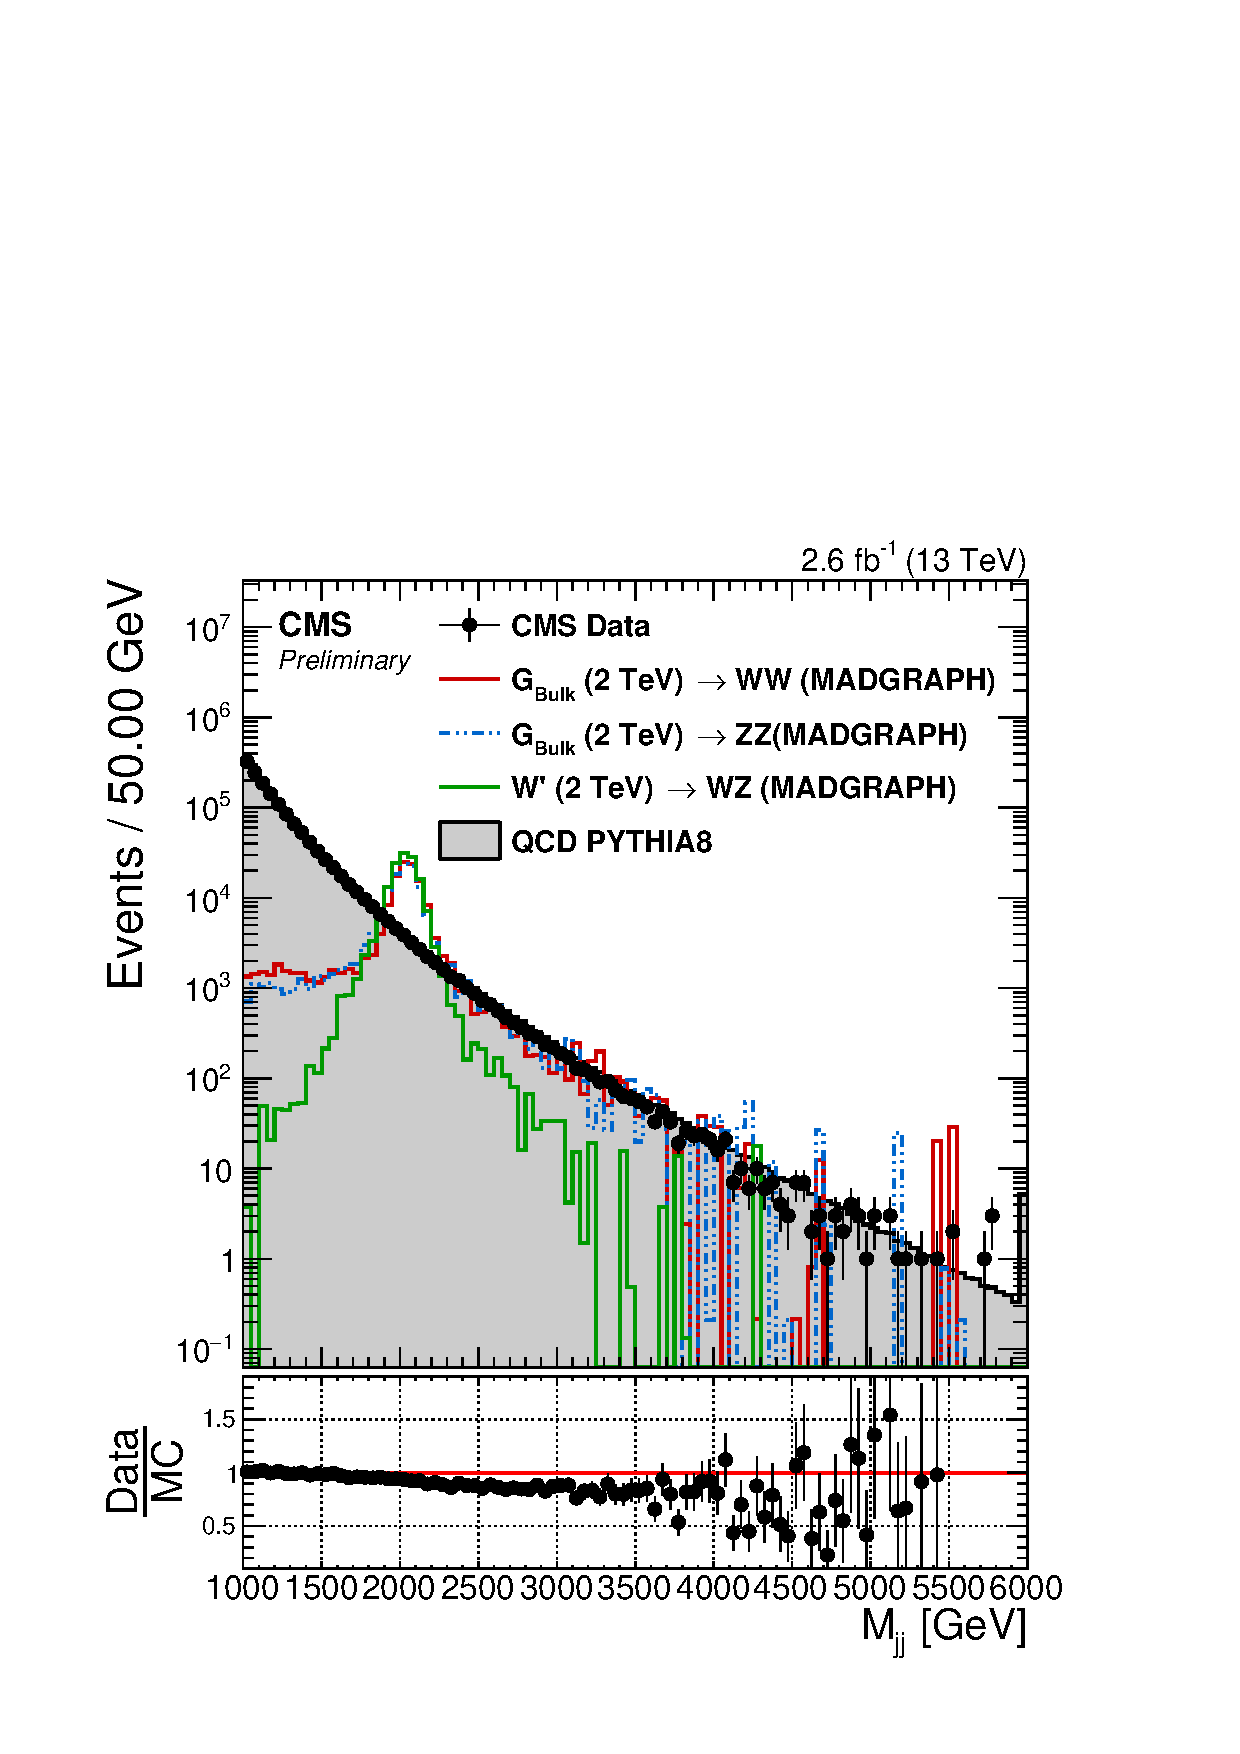
\includegraphics[width=0.4\textwidth]{figures/analysis/search1/AN-15-211/controlplots/silverjson/Mjj_WSignal.pdf}
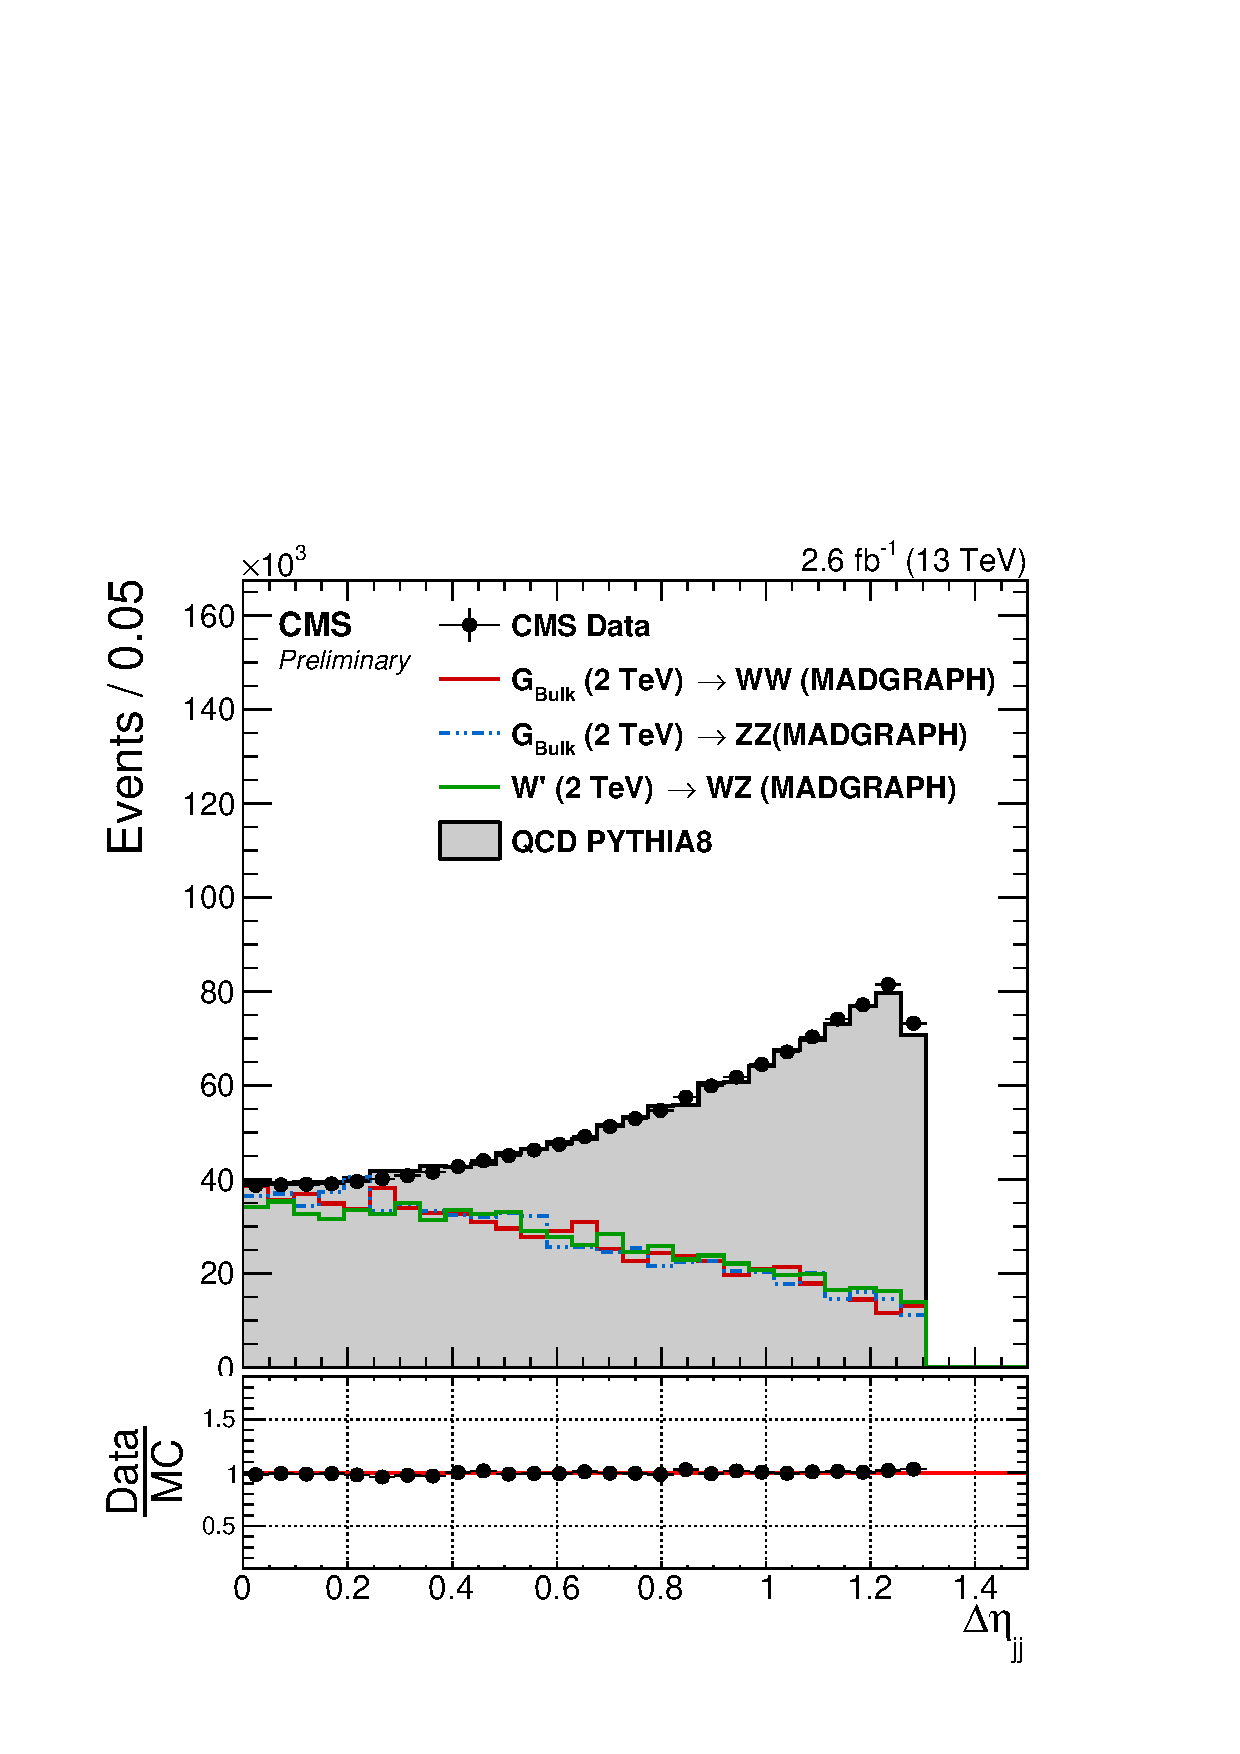
\includegraphics[width=0.4\textwidth]{figures/analysis/search1/AN-15-211/controlplots/silverjson/DeltaEta_WSignal.pdf}
\caption{Jet \PT (top left), $\eta$ (top right), dijet invariant mass (bottom left) and $|\Delta \eta|_{jj}$ (bottom right) distribution for the two leading jets in the event after loose preselections are applied. The signal is scaled by an arbitrary number.}
\label{fig:kinematics-all}
\end{figure}

\subsection{Vector boson tagging}
\label{sec:searchI:wtagging}
After preselections, we take advantage of the jet substructure algorithms described in Section~\ref{sec:objreco:substructure} to further separate boosted W/Z jets from the QCD multijet background. In the 8 \TeV analysis~\cite{Khachatryan:1700394} published the previous year, the pruning algorithm was the chosen grooming algorithm of CMS. However, recent progress had been made in the development of alternative grooming algorithms that had favorable properties from a theoretical point of view (see Sections~\ref{sec:objreco:grooming} and ~\ref{sec:searchII:puppisoftdrop}). We therefore studied two different grooming algorithms: pruning and softdrop (with $\beta=0$ and $z_{cut} = 0.1$). A comparison of the jet mass for W, Z, and H jets after either the softdrop (dotted lines) or pruning (solid lines) algorithms were applied is shown in Figure~\ref{fig:searchI:sdvspruning}.
 \begin{figure}[h!]
 \centering
 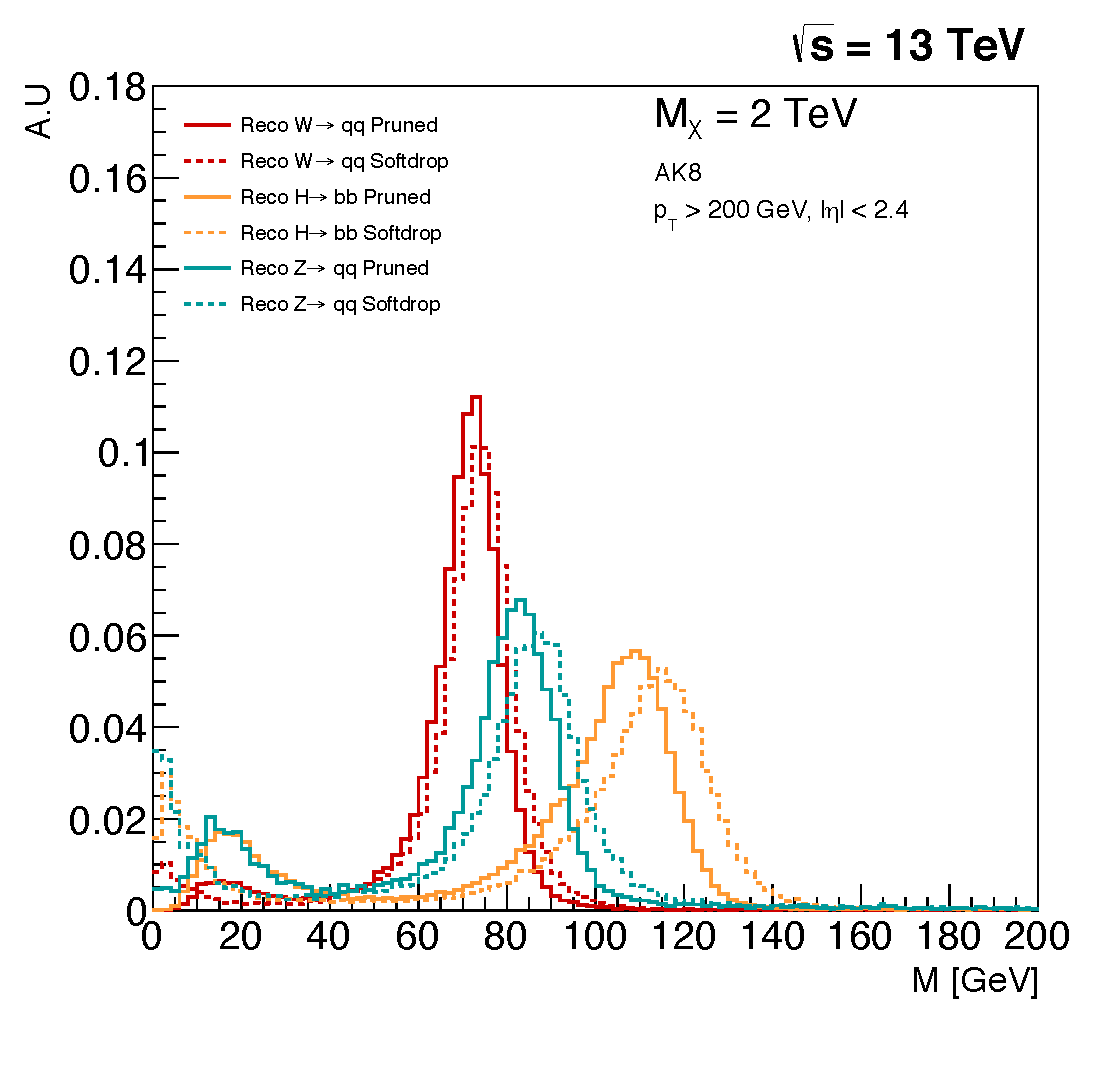
\includegraphics[width=0.49\textwidth]{figures/analysis/search1/misc/SDvsPruned.pdf}
 \caption{The softdrop (dotted lines) and the pruned (solid lines) jet mass for \PW, \PZ and \PH jets.}
 \label{fig:searchI:sdvspruning}
 \end{figure}
One of the first observations we made comparing the two grooming algorithms was that there appeared to be a strong dependence of the softdrop mass on the jet \PT. Figure~\ref{fig:searchI:grommedmassshift} shows the pruned (left) and softdrop (right) mass distributions for \PW jets coming from the decay of a \BulkG with a resonance mass of $0.8 \TeV < \mX < 4 \TeV$. While the pruned jet mass mean appeared stable as the jet transverse momenta of the jet increased ($\PT\sim\mX/2$), the mean of the softdrop jet mass shifted towards lower values as jet \PT increased.
\begin{figure}[h!]
\centering
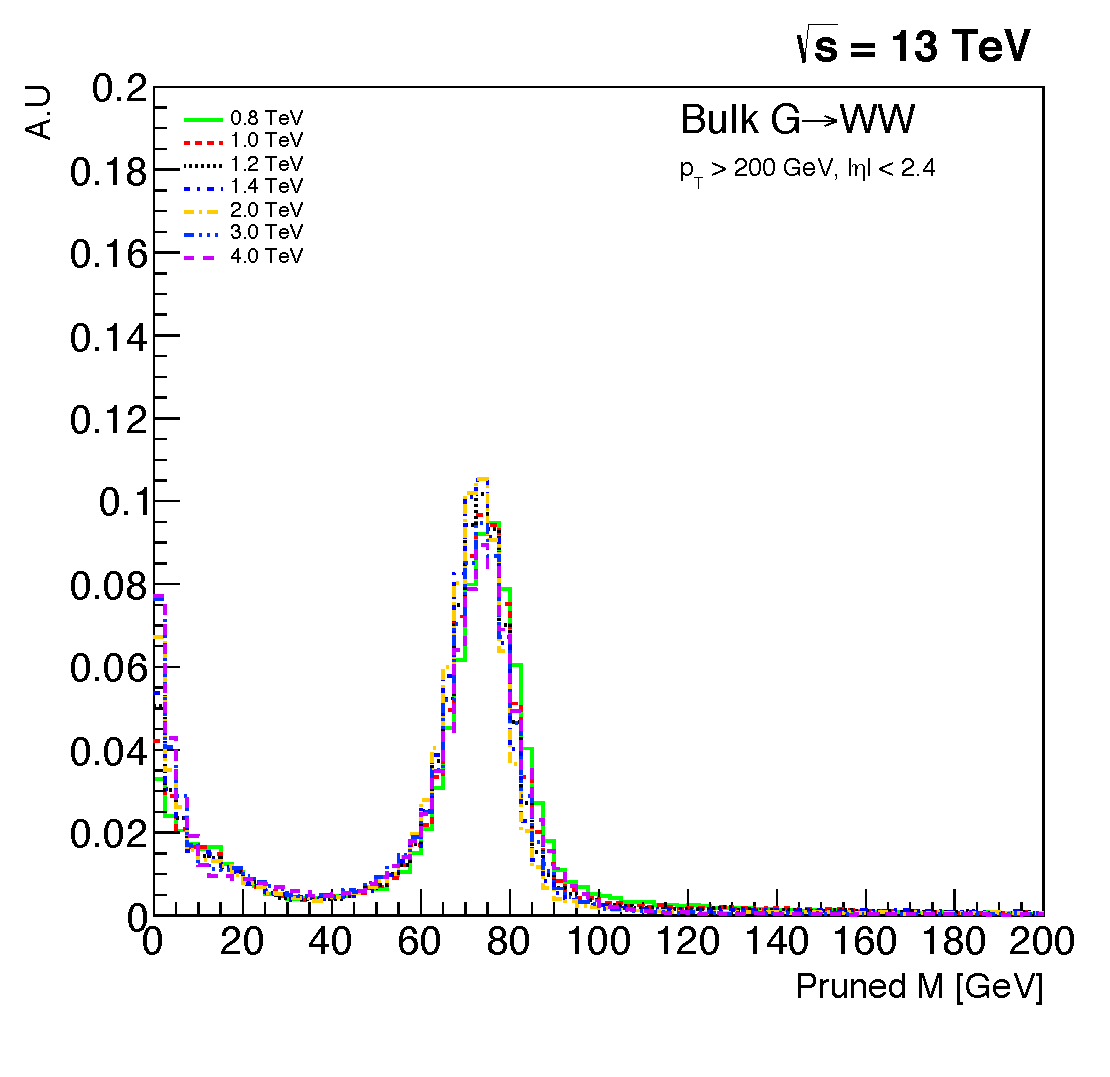
\includegraphics[width=0.49\textwidth]{figures/analysis/search1/misc/pruned_mass_shift.pdf}
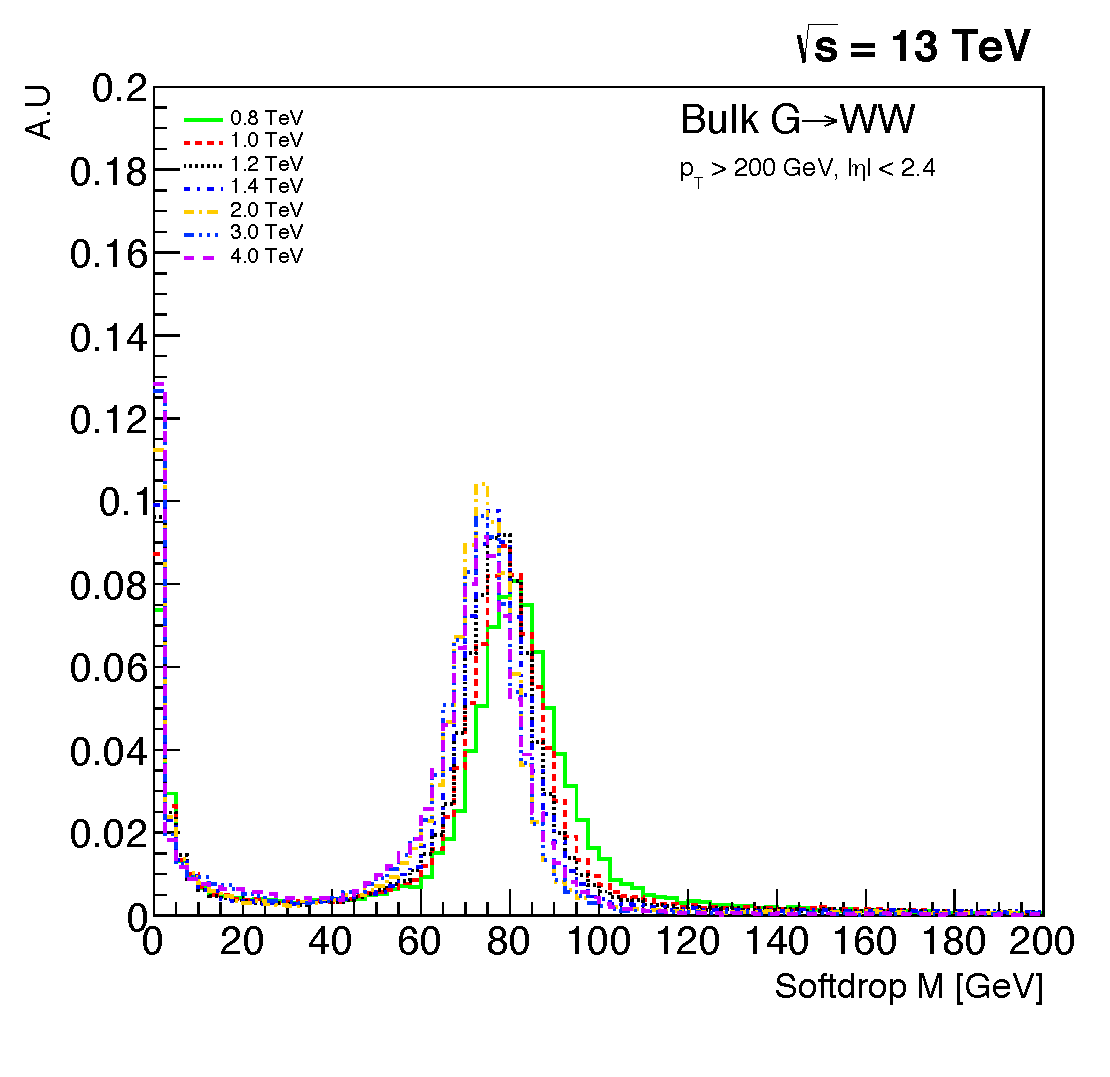
\includegraphics[width=0.49\textwidth]{figures/analysis/search1/misc/softdrop_mass_shift.pdf}
\caption{The jet mass distribution for W jets coming from a $\textrm{G}_{\textrm{bulk}}$ of masses in the range $0.8 \TeV < \mX < 4 \TeV$ decaying to \WW, here with pruning applied (left) and softdrop (right). A strong shift in the jet mass mean as a function of \PT ($\sim\mX/2$), is observed for jets groomed with the softdrop algorithm. Charge hadron subtraction is applied to all jets before clustering.}
\label{fig:searchI:grommedmassshift}
\end{figure}
In order to investigate whether this was a reconstruction effect or an algorithmic effect, we additionally looked at the pruned and softdrop mass for generator-level jets (jets clustered with generator-level particles not passed through the detector simulation). Figure~\ref{fig:searchI:grommedmassshift_genvsreco} shows the reconstructed (solid line) and generator-level (dotted line) jet mass distributions after pruning (left) or softdrop (right) have been applied. Again, the distributions are compared for jets with very different \PT profiles, here for W jets coming from a $\BulkG \rightarrow \WW$ of mass 0.8 \TeV (red) yielding a \PT of about 400 GeV, and a mass of 2.0 TeV, yielding a \PT of about 1 TeV. Interestingly, we observe a \PT-dependent mass shift already for generator level softdrop jets (comparing the dotted lines in the right plot), an effect further enhanced at reconstruction level. This effect is not present for pruned jets, for either generator level or reconstruction level.
\begin{figure}[h!]
\centering
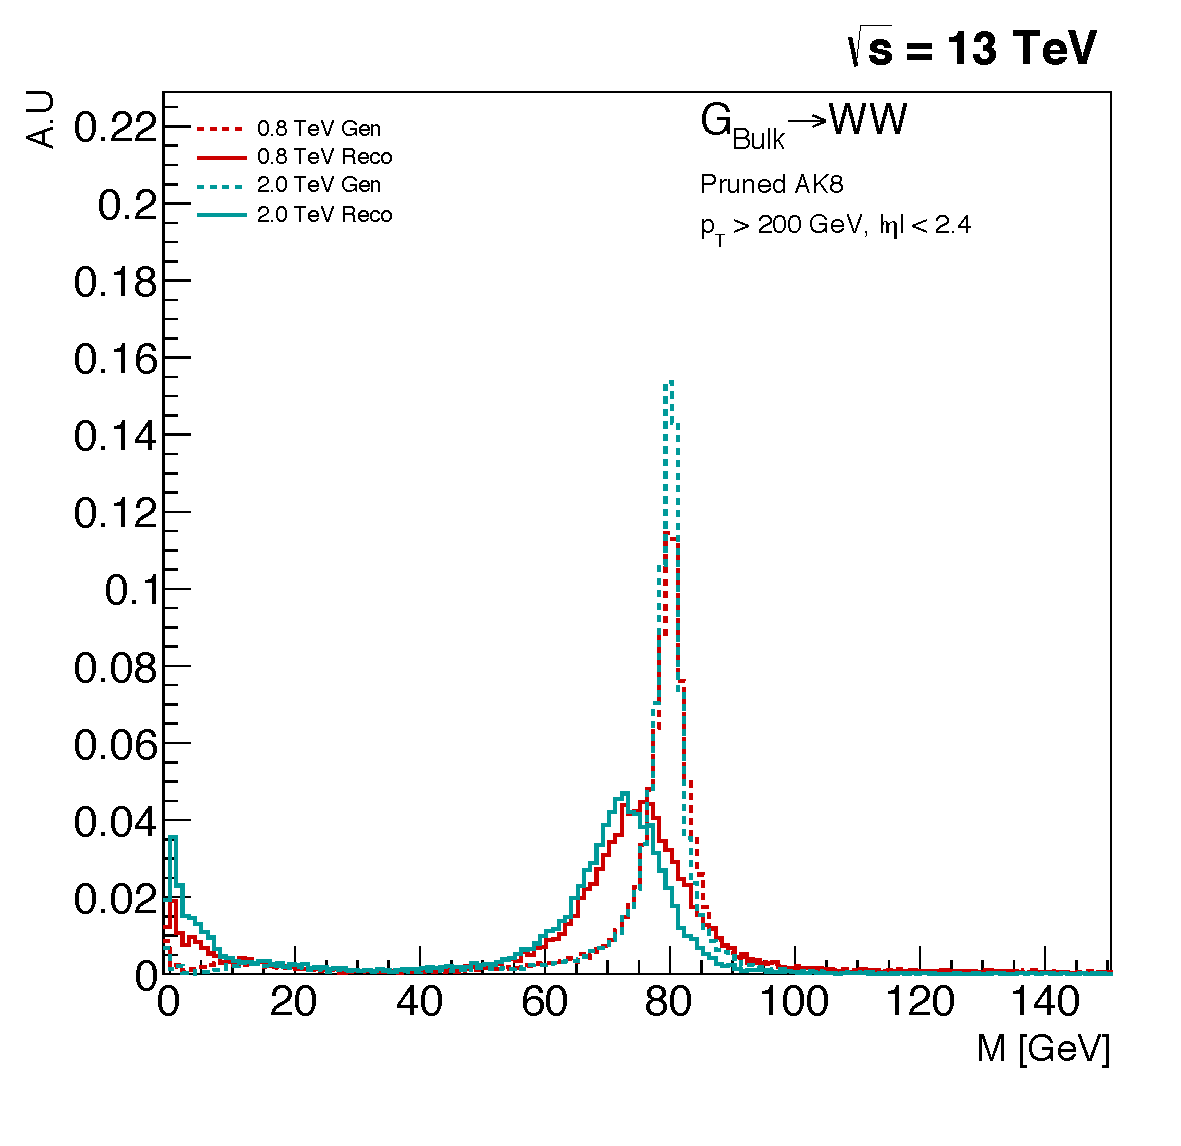
\includegraphics[width=0.49\textwidth]{figures/analysis/search1/misc/pruned_mass_shift_genvsreco.pdf}
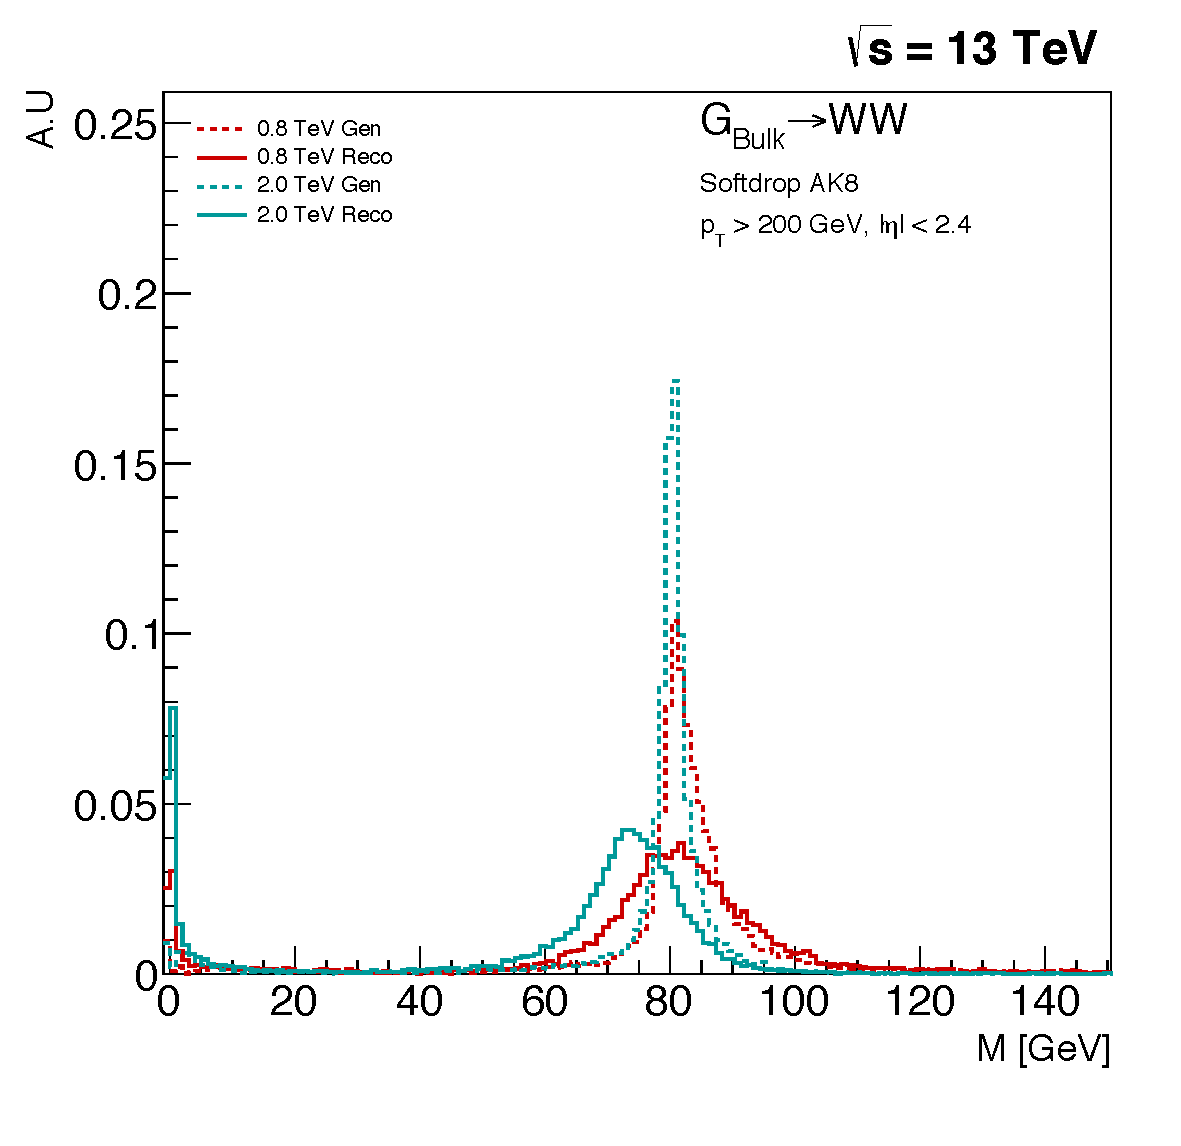
\includegraphics[width=0.49\textwidth]{figures/analysis/search1/misc/softdrop_mass_shift_genvsreco.pdf}
\caption{The reconstructed (solid line) and generator level (dotted line) jet mass distribution for W jets coming from a $\BulkG \rightarrow \WW$ of mass $\mX = 0.8 \TeV$ (red), roughly $\PT\sim 400 \GeV$, and $\mX = 2.0 \TeV$ (blue), $\PT\sim 1 \TeV$. Here for the pruned (left) and softdrop (right) jet mass.}
\label{fig:searchI:grommedmassshift_genvsreco}
\end{figure}
The observed \PT-dependence of the softdrop mass was problematic due to the fact that it would require a \PT-dependent mass window. This would again require several different measurements to produce an efficiency scale factor between simulation and data, for each mass window, or a significantly higher uncertainty on the signal yield. Due to these findings, the grooming algorithm of choice for this analysis is pruning, with the signal selection window defined as $65 \GeV < m_{p} < 105 \GeV$. The above findings will be important for subsequent analyses and are revisited in Section~\ref{searchII}.\par
The variable used to determine the substructure of the V jets is the n-subjettiness ratio \nsubj, as described in Section~\ref{sec:objreco:nsubj}. The \nsubj variable is correlated to the pruned jet mass, however, it still provides additional signal discrimination when applied after the pruned jet mass selection. Figure~\ref{fig:searchI:tau21_groomedvsungroomed} shows the \nsubj distribution for the QCD background and W jets from a signal decay before (left) and after (right) a pruned mass cut of $65 \GeV < m_{p} < 105 \GeV$ has been applied.
\begin{figure}[h!]
\centering
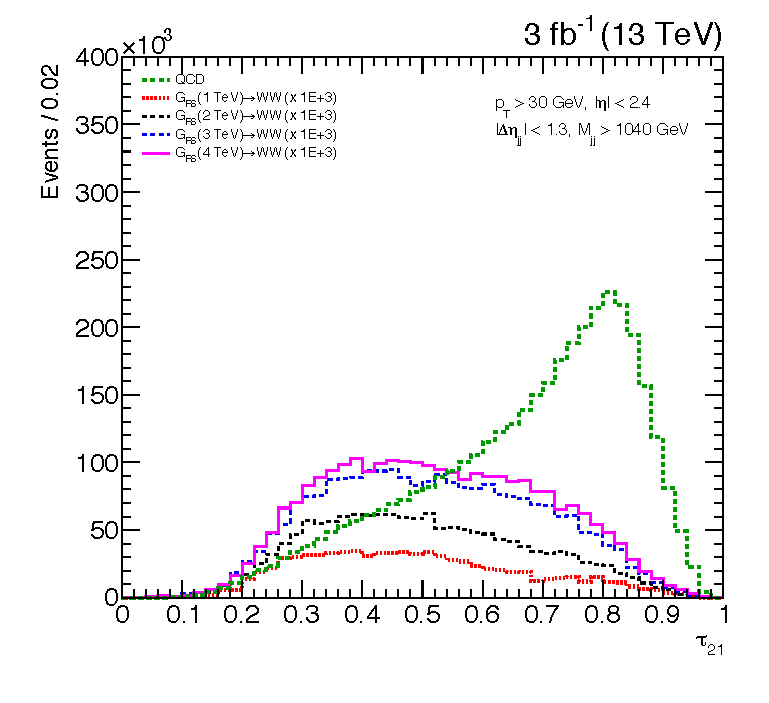
\includegraphics[width=0.49\textwidth]{figures/analysis/search1/misc/tau21_ungroomed.pdf}
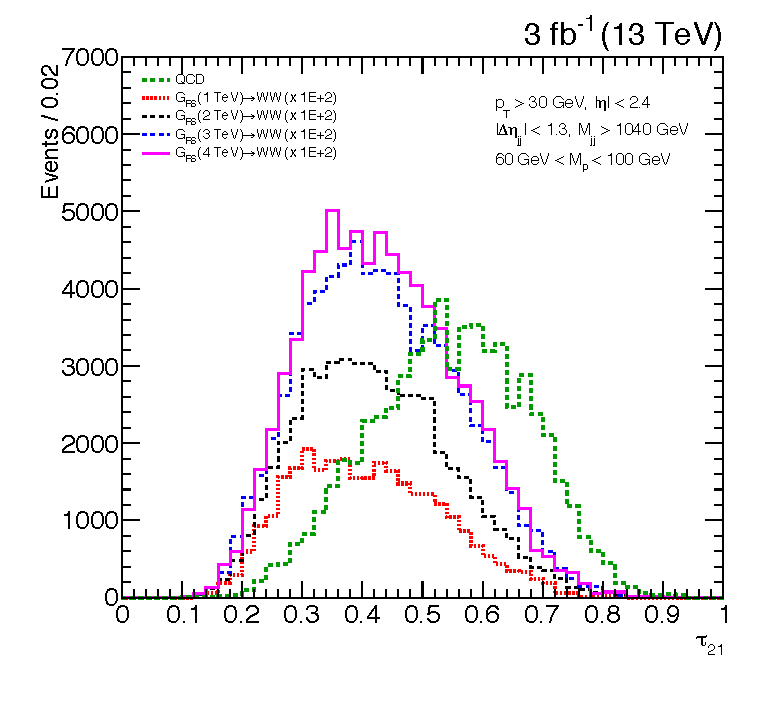
\includegraphics[width=0.49\textwidth]{figures/analysis/search1/misc/tau21_groomed.pdf}
\caption{The \nsubj distribution for QCD background and signal jets before (left) and after (right) a pruned mass window is applied. The discriminating power of \nsubj is strongly reduced after grooming.}
\label{fig:searchI:tau21_groomedvsungroomed}
\end{figure}
\noindent We perform a cut optimization on \nsubj after all analysis selections, including the pruned mass window of $65 \GeV < m_{p} < 105 \GeV$, have been applied. This is done by scanning over thresholds for the \nsubj variable, and for each threshold, computing the Punzi significance~\cite{Punzi:2003bu} defined as
\begin{equation*}
\textrm{S} = \frac{\epsilon_S}{1+\sqrt{\textrm{B}}}  ,
\end{equation*}  
where $\epsilon_S$ is the signal efficiency and B is the total number of background events. The selection with the highest significance is defined as the optimal value. The signals under consideration are W jets coming from the decay of a \BulkG with $1 \TeV< mX < 4 \TeV$, against a background of light-flavored QCD jets. Only jets with a dijet invariant mass in a 20\% window around the resonance mass are considered. The Punzi significance as a function of the upper cut value on \nsubj is shown on the left in Figure~\ref{fig:searchI:tau21_punzi}.
\begin{figure}[h!]
\begin{center}
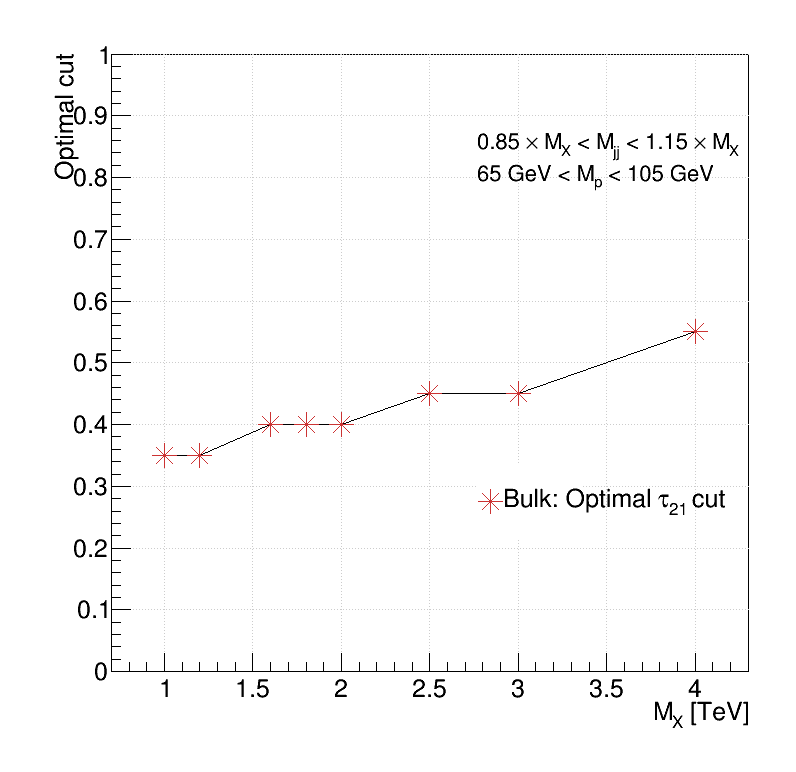
\includegraphics[width=0.49\textwidth]{figures/analysis/search1/AN-15-196/tau21optimisation/HP_Punzi_BulkWW.png}
%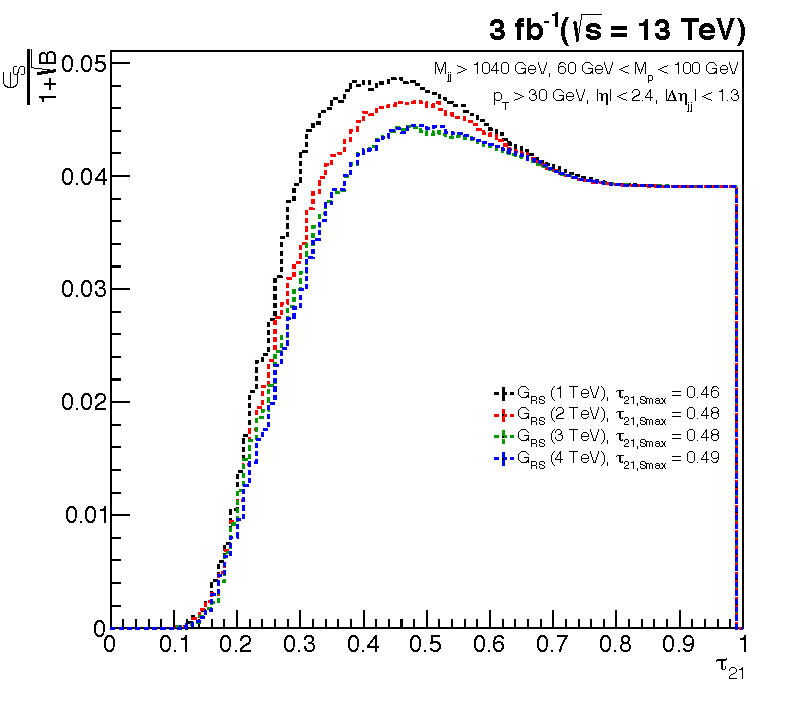
\includegraphics[width=0.49\textwidth]{figures/analysis/search1/misc/tau21_punzi.pdf}
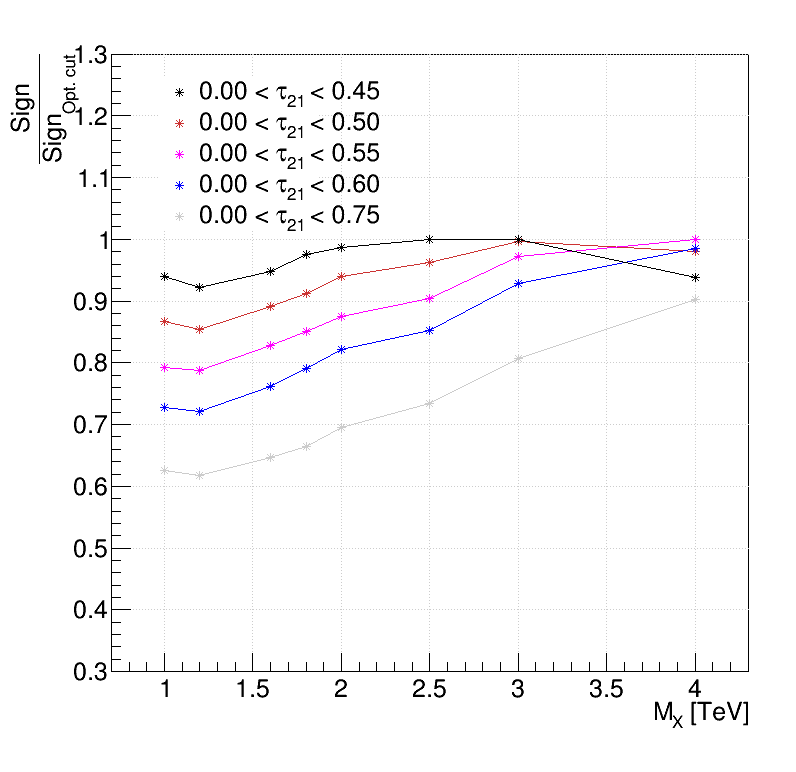
\includegraphics[width=0.49\textwidth]{figures/analysis/search1/AN-15-196/tau21optimisation/HP_CutSignificance_bulkWW.png}\\
\caption{Left: Optimal upper value of \nsubj for selecting the signal as a function of \BulkG mass. Right: The ratio of a given \nsubj cut over the significance of the best cut at that mass value.}
\label{fig:searchI:tau21_punzi}
\end{center}
\end{figure}
The optimal cut gets looser as the dijet invariant mass increases, something which can be understood when looking at the QCD dijet invariant mass spectrum in Figure~\ref{fig:kinematics-all}. The number of QCD jets falls off exponentially with \mjj, meaning that the background at 4 \TeV is considerably lower than at 1 \TeV. This allows for a looser cut on \nsubj as \mjj increases. In order to choose a single cut which works reasonably well for all values of resonance mass, we look at the ratio of a given \nsubj cut over the significance of the best cut at that mass value. This is shown in the right plot of Figure~\ref{fig:searchI:tau21_punzi}. Choosing signal events with a $\nsubj < 0.45$ yields the most stable performance out of the investigated \nsubj selection requirements and also maintains low background rates at low \mjj. This selection is therefore used for our main analysis category. In order to account for the fact that background rates are lower for higher values of \mjj, we add an additional analysis category, $0.45 < \nsubj < 0.75$, which contains $>95\%$ of the signal and enhances the analysis sensitivity in the case when the background is low. These categories are hereafter referred to as the \emph{high-purity} (HP) category, for jets with $0<\tau_{21} \leq 0.45$, and the \emph {low-purity} (LP) category, for jets with $0.45<\tau_{21}\leq0.75$. QCD jets from light-flavor quarks and gluons (u,d,s,g) can be incorrectly identified as W-jets, and these events are referred to as "mistags" of the W-tagger. The W-tagging efficiency and QCD light-flavored jet mistagging rate for a W-tagger consisting of $0<\tau_{21} \leq 0.45$ and  $65 \GeV < m_{p} < 105 \GeV$ is shown in Figure~\ref{fig:searchI:wtageff}, both as a function of jet \PT and as a function of number of primary vertices in the event.
\begin{figure}[h]
\begin{center}
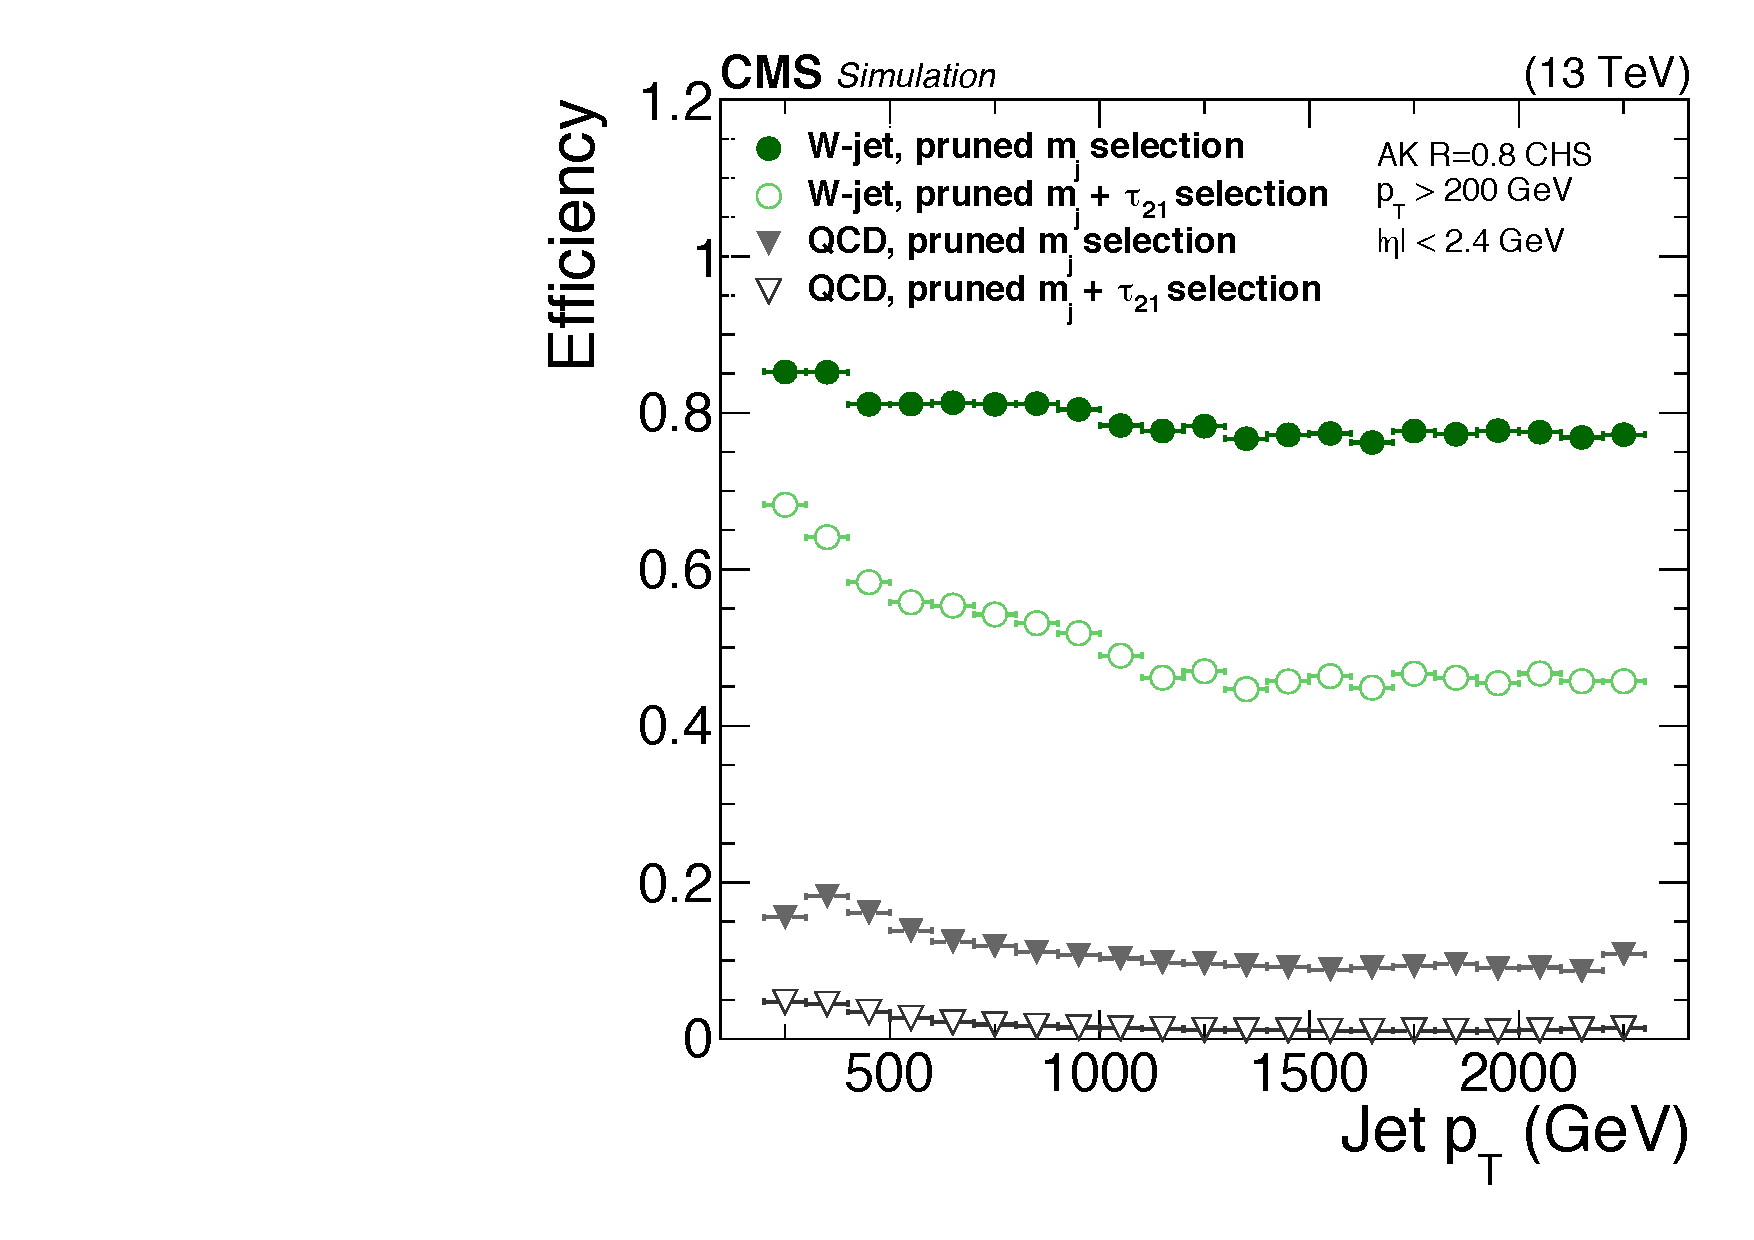
\includegraphics[width=0.49\textwidth]{figures/analysis/search1/misc/WtagSigEff_vpT_pruned.pdf}
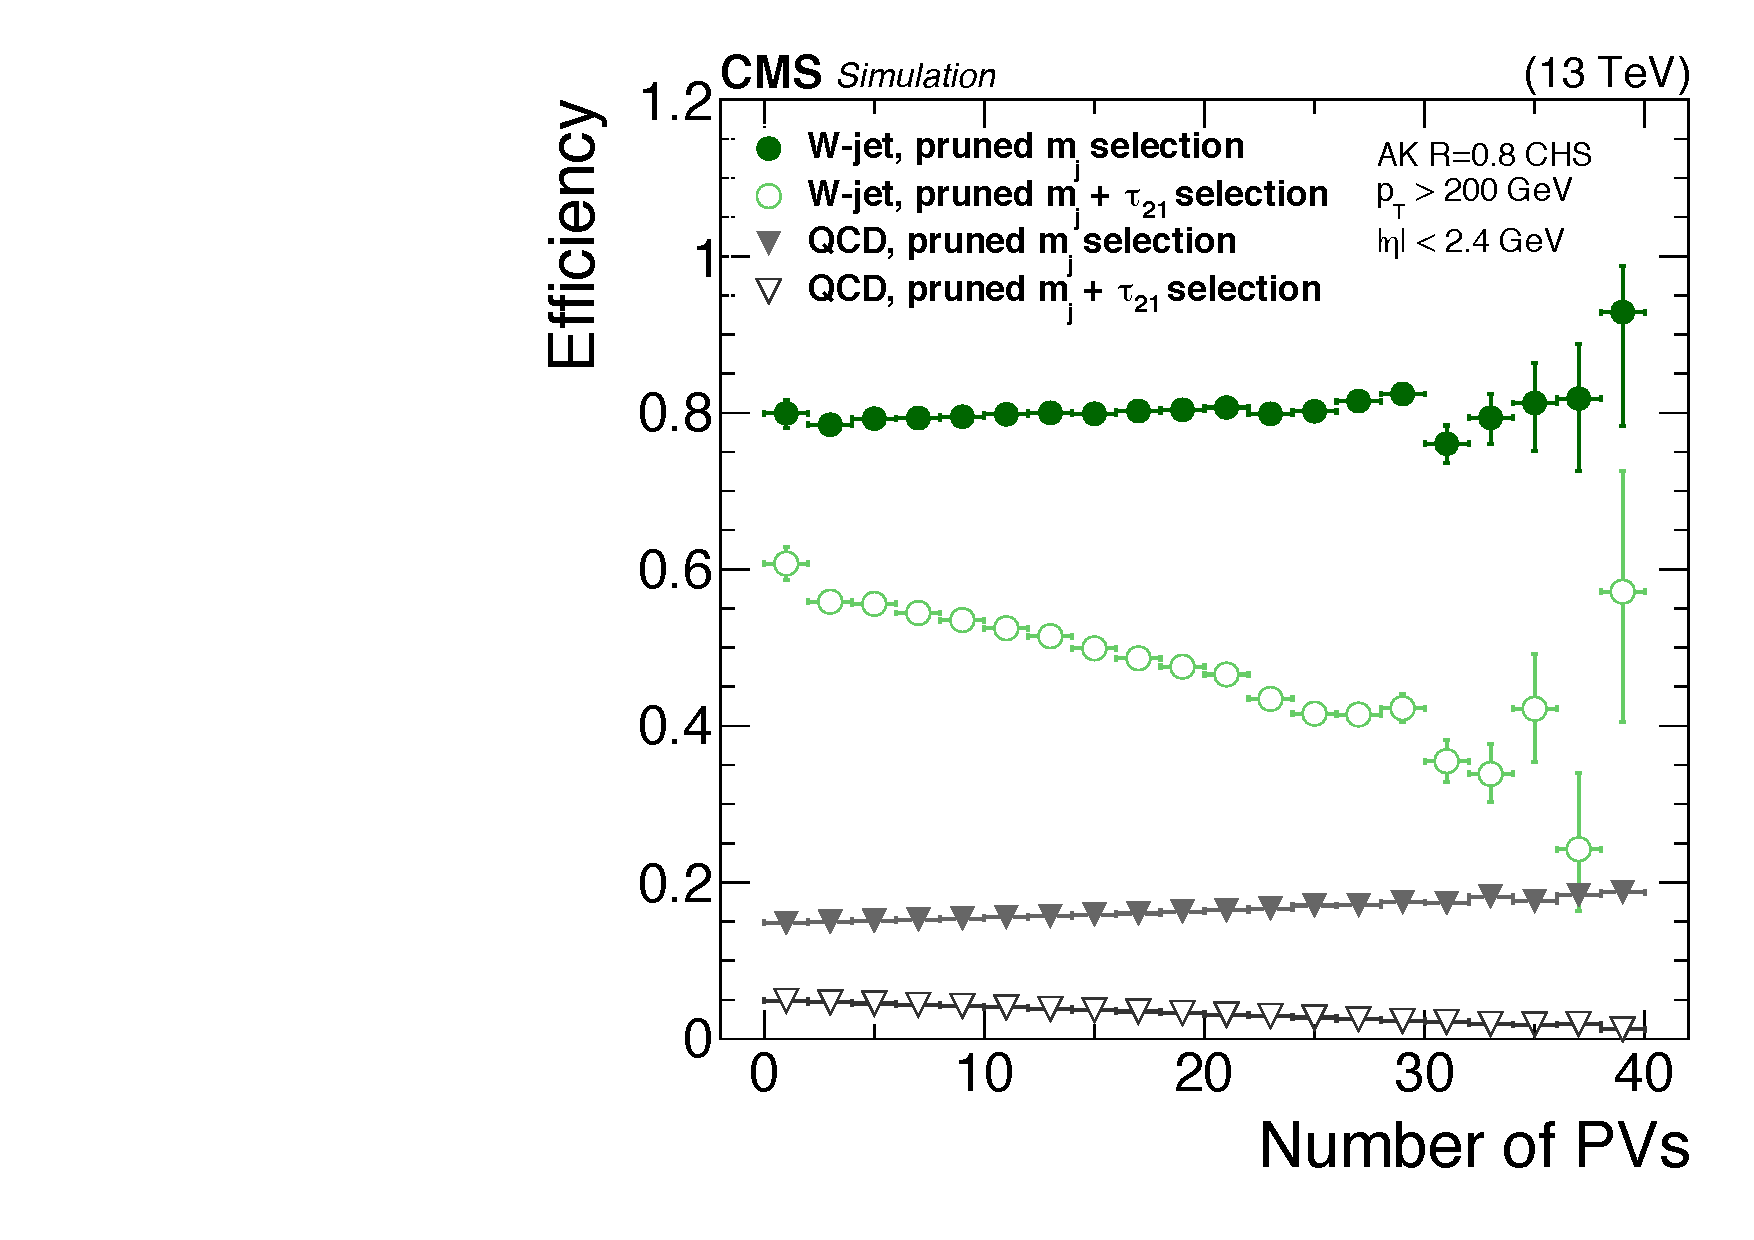
\includegraphics[width=0.49\textwidth]{figures/analysis/search1/misc/WtagSigEff_vnPVs_pruned.pdf}
\caption{The W-tagging efficiency (green) and light jet mistag rate (grey) for a selection based on either the pruned jet mass or the pruned jet mass and \nsubj as a function of \PT (left) and the number of primary vertices (right).}
\label{fig:searchI:wtageff}
\end{center}
\end{figure}
The signal efficiency when applying only the pruned jet mass selection is around 80\% with a mistag rate of $\sim 15\%$. After applying the \nsubj selection, the signal efficiency drops to around 55\% and the mistagging rate to $\sim 2\%$. Another interesting feature is the dependence of \nsubj on jet \PT and pileup, compared to the resilience of the groomed mass as a function of the same variables. This will be another feature we explore in the second analysis (Section~\ref{searchII}). Figure~\ref{fig:wtag} shows the pruned jet mass (left) and the $\tau_{21}$ distribution (right) for signal and background Monte Carlo, as well as the distributions measured in data. 
\begin{figure}[h!]
\centering
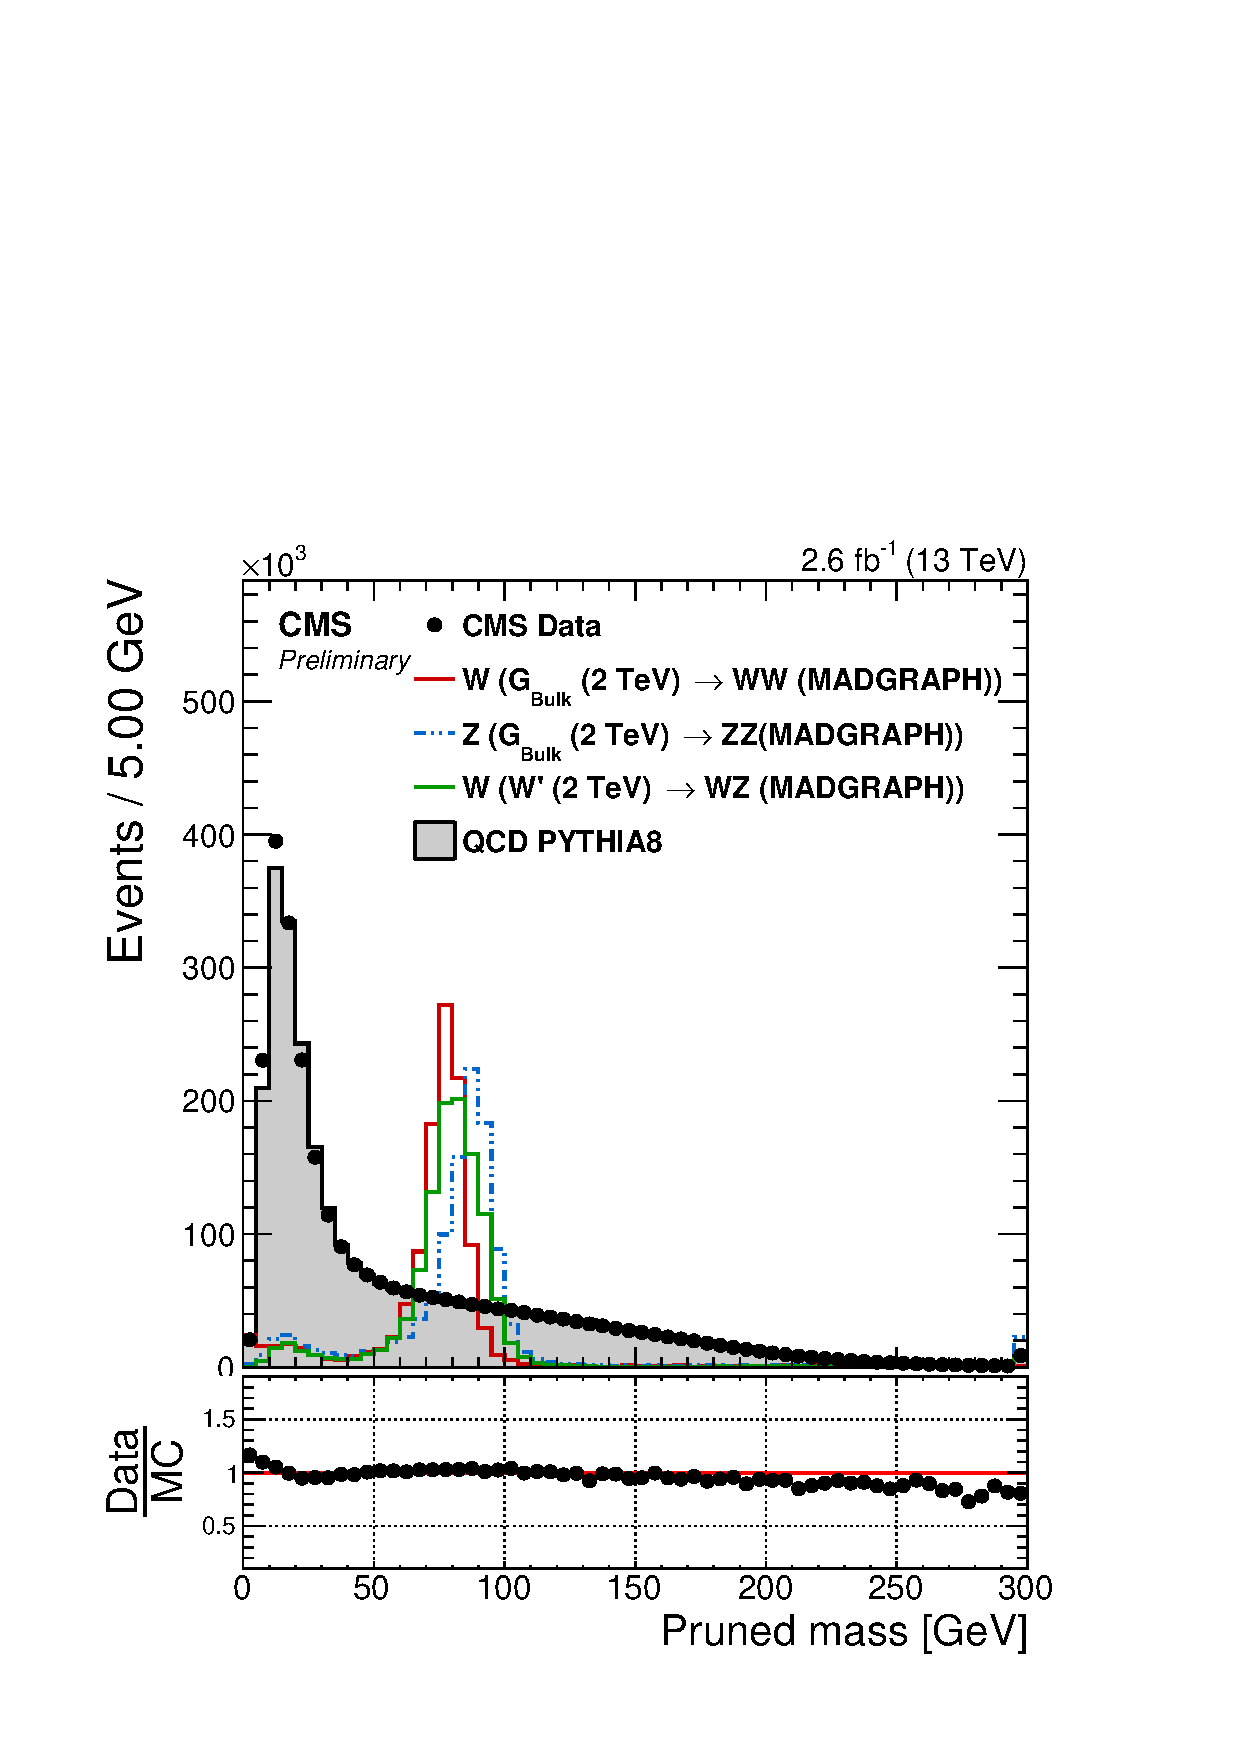
\includegraphics[width=0.4\textwidth]{figures/analysis/search1/AN-15-211/controlplots/silverjson/PrunedMass_WSignal.pdf}
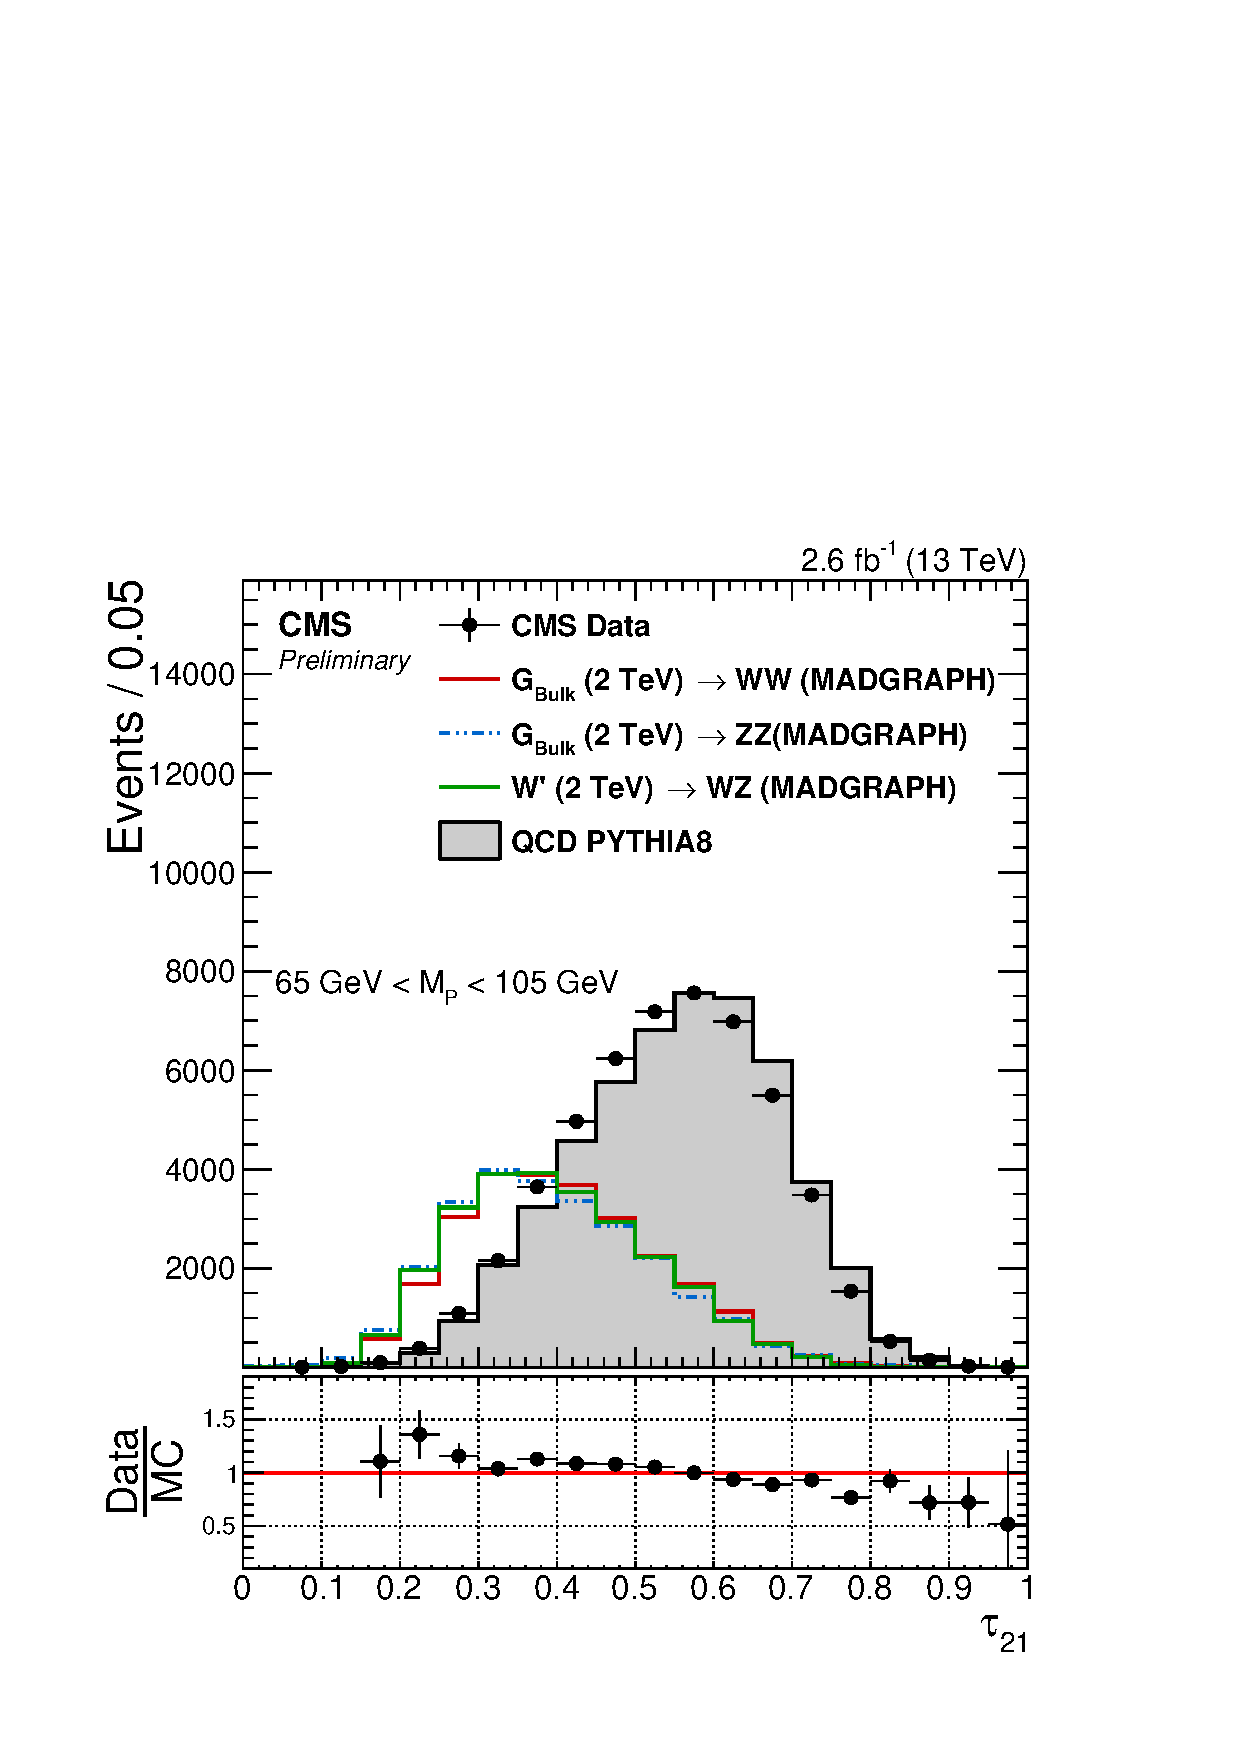
\includegraphics[width=0.4\textwidth]{figures/analysis/search1/AN-15-211/controlplots/silverjson/Tau21_punzi_WSignal.pdf}\\
\caption{Pruned jet mass (left) and $\tau_{21}$ (right) distributions for data and simulated samples. Simulated samples are scaled to match the distribution in data. The $\tau_{21}$ distribution is shown for jets after a cut on the pruned jet mass of $65 {\GeV} < m_{p} < 105 {\GeV}$ has been applied.}
\label{fig:wtag}
\end{figure}

\subsection{Analysis categorization}
As the analysis requires two W/Z-tags, we always require one HP-tagged jet and then divide into LP and HP categories depending on whether the other jet is of high or low purity. In addition, in order to further enhance the analysis sensitivity, we further split the pruned jet mass window into a W and a Z boson window where the W window is defined as $65 {\GeV} < m_{p} < 85 {\GeV}$ and the Z boson window as $85 {\GeV} < m_{p} < 105 {\GeV}$. This has the added benefit of allowing us to discriminate between a \BulkG decaying to \WW or \ZZ, and a \PWpr decaying into \WZ by separating these events into categories. The signal yield will be higher in the WZ category for a \PWpr decaying to a W and Z boson than for a \BulkG decaying to \WW or \ZZ. Figure~\ref{fig:searchI:massCatWpr} shows the relative expected signal yield (left) and expected limits (left) in the different mass categories for a \PWpr with a mass of 2 TeV.
 \begin{figure}
 \centering
 \begin{minipage}{0.5\textwidth}
 \centering
 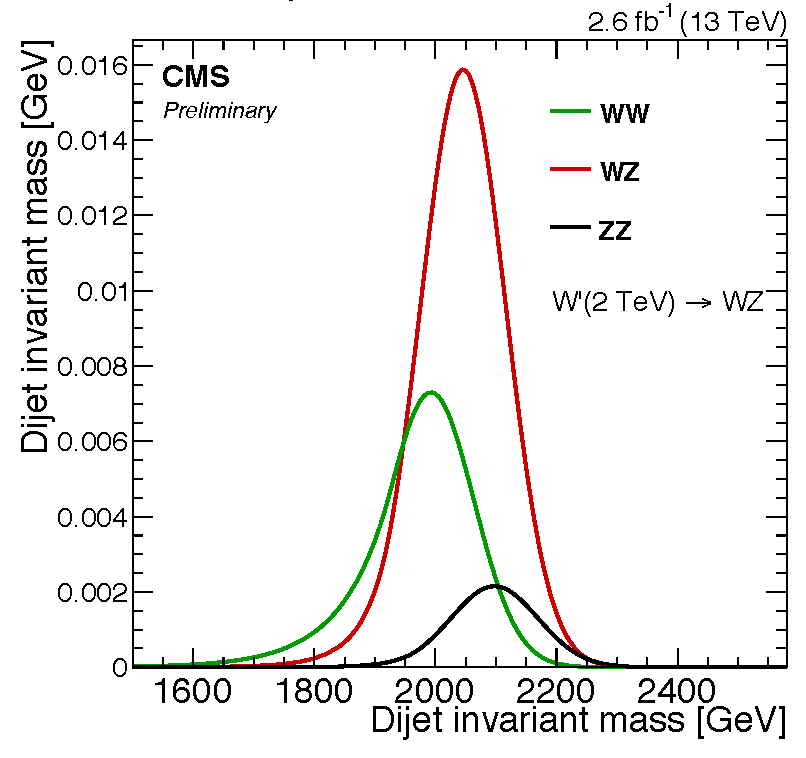
\includegraphics[width=0.99\textwidth]{figures/analysis/search1/misc/massCategories.pdf}
 \end{minipage}
 \begin{minipage}{0.29\textwidth}
 \centering
 \captionsetup{type=table} %% tell latex to change to table
 \begin{tabular}{| l | c |}
 \hline
 \multicolumn{2}{|c|}{$\PWpr (2 \TeV) \rightarrow \WZ$}\\
 \hline
 Category & Expected limit \\
 \hline
 WWHP & 2.1984 \\ 
 WWLP & 2.3261 \\ 
 WZHP & 1.2419 \\ 
 WZLP & 1.7157 \\ 
 ZZHP & 7.0855 \\ 
 ZZLP & 9.2012 \\ 
 \hline
 \end{tabular}
 \end{minipage}
 \caption{The expected signal yield per mass category for a \PWpr (2 \TeV) decaying to a \PW and a \PZ (left) together with the expected limit per mass category for the same signal (right).}
 \label{fig:searchI:massCatWpr}
 \end{figure}
All categories are combined in the end, leading to the same or better sensitivity at each resonance mass value than when using the whole pruned mass window. Figure~\ref{fig:searchI:massCategories} shows the expected 95\% CL upper limits on the production cross section of a \PWpr decaying to \WZ (left) and a \BulkG decaying to \WW (right) as a function of the resonance mass in the HP category. The blue line corresponds to the expected limits obtained when not splitting into mass categories and the red line corresponds to the limit using the combination of two categories. The dotted and solid black lines are the limits for the \PW and \PZ categories, respectively. The combination of two mass categories leads to slightly better (~10\%) or similar sensitivity as when using one large mass window.
\begin{figure}[h!]
 \centering
 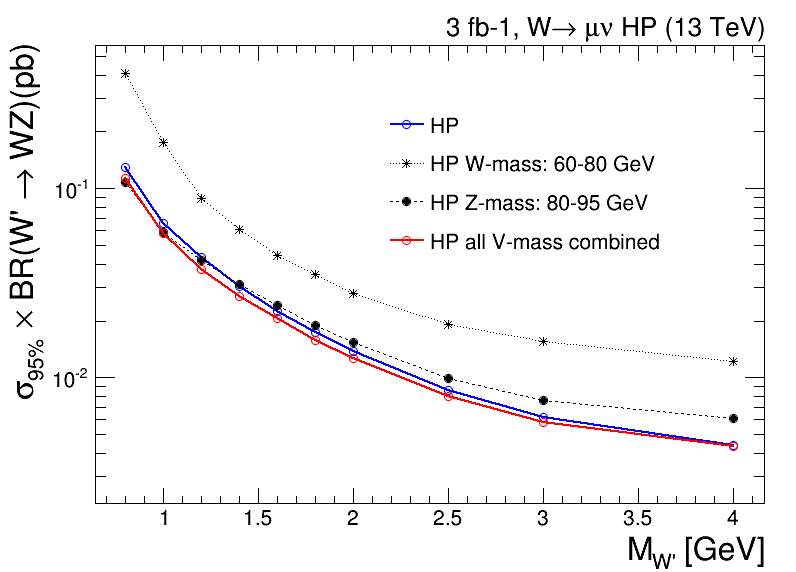
\includegraphics[width=0.49\textwidth]{figures/analysis/search1/AN-15-196/massCategories/compare-HP-HPV-Wprime.png}
  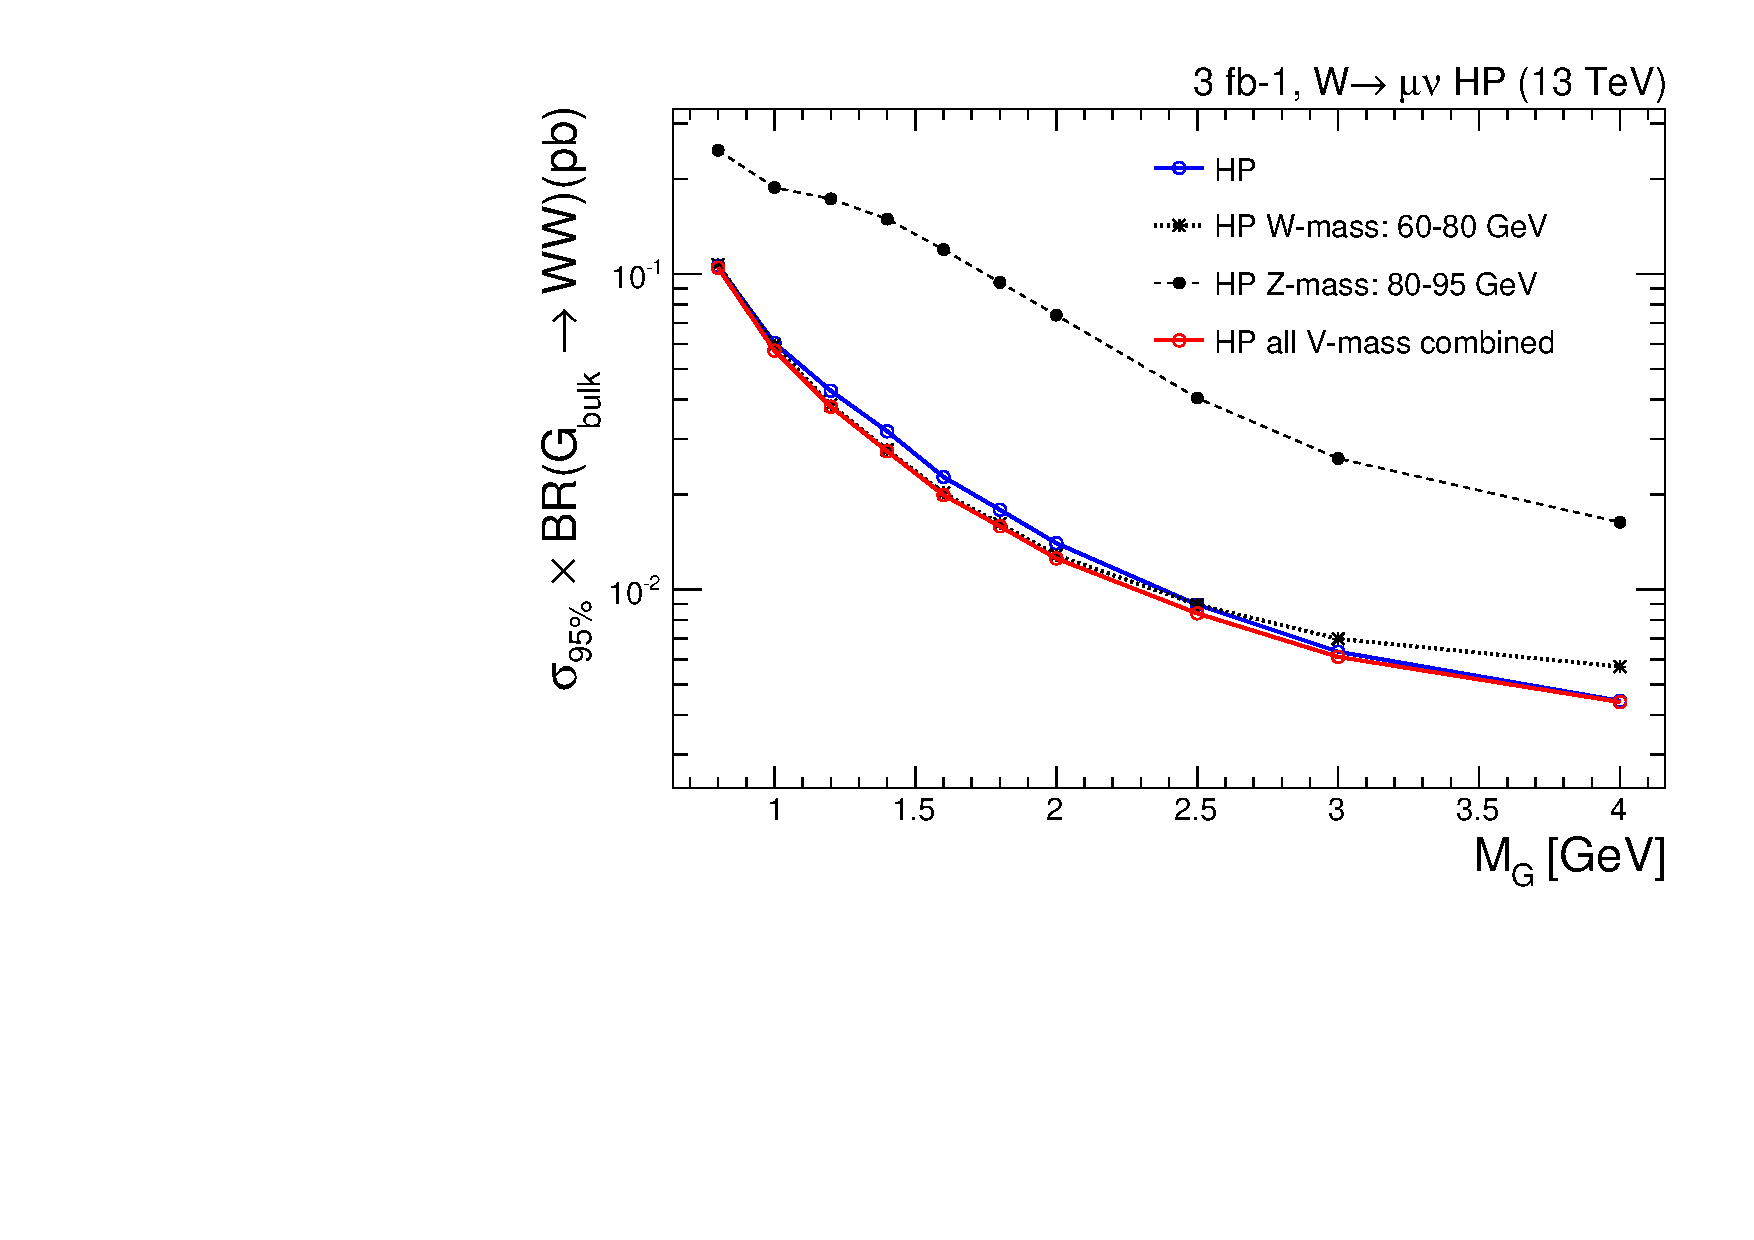
\includegraphics[width=0.49\textwidth]{figures/analysis/search1/AN-15-196/massCategories/compare-HP-HPV-BulkG.pdf}
 \caption{Expected 95\% CL upper limits on the production cross section of a \PWpr (left) and \BulkG (right) signal as a function of the resonance mass for the different mass categories for events passing the high-purity $\tau_{21}$ selection.}
 \label{fig:searchI:massCategories}
 \end{figure}
 The real benefit of splitting into mass categories becomes obvious when defining a test statistics based on the likelihood ratios of each signal hypothesis, $q = -2 \ln(L_{\BulkG}/L_{\PWpr})$, shown in Figure~\ref{fig:searchI:signalsep}. For a signal with a signal strength corresponding to a 3-4 $\sigma$ excess, the test statistics for each signal hypothesis are well separated ($\sim3.5 \sigma$), allowing us to make a statement of whether a possible signal is more likely due to a \BulkG or a \PWpr particle.
\begin{figure}[h!]
 \centering
 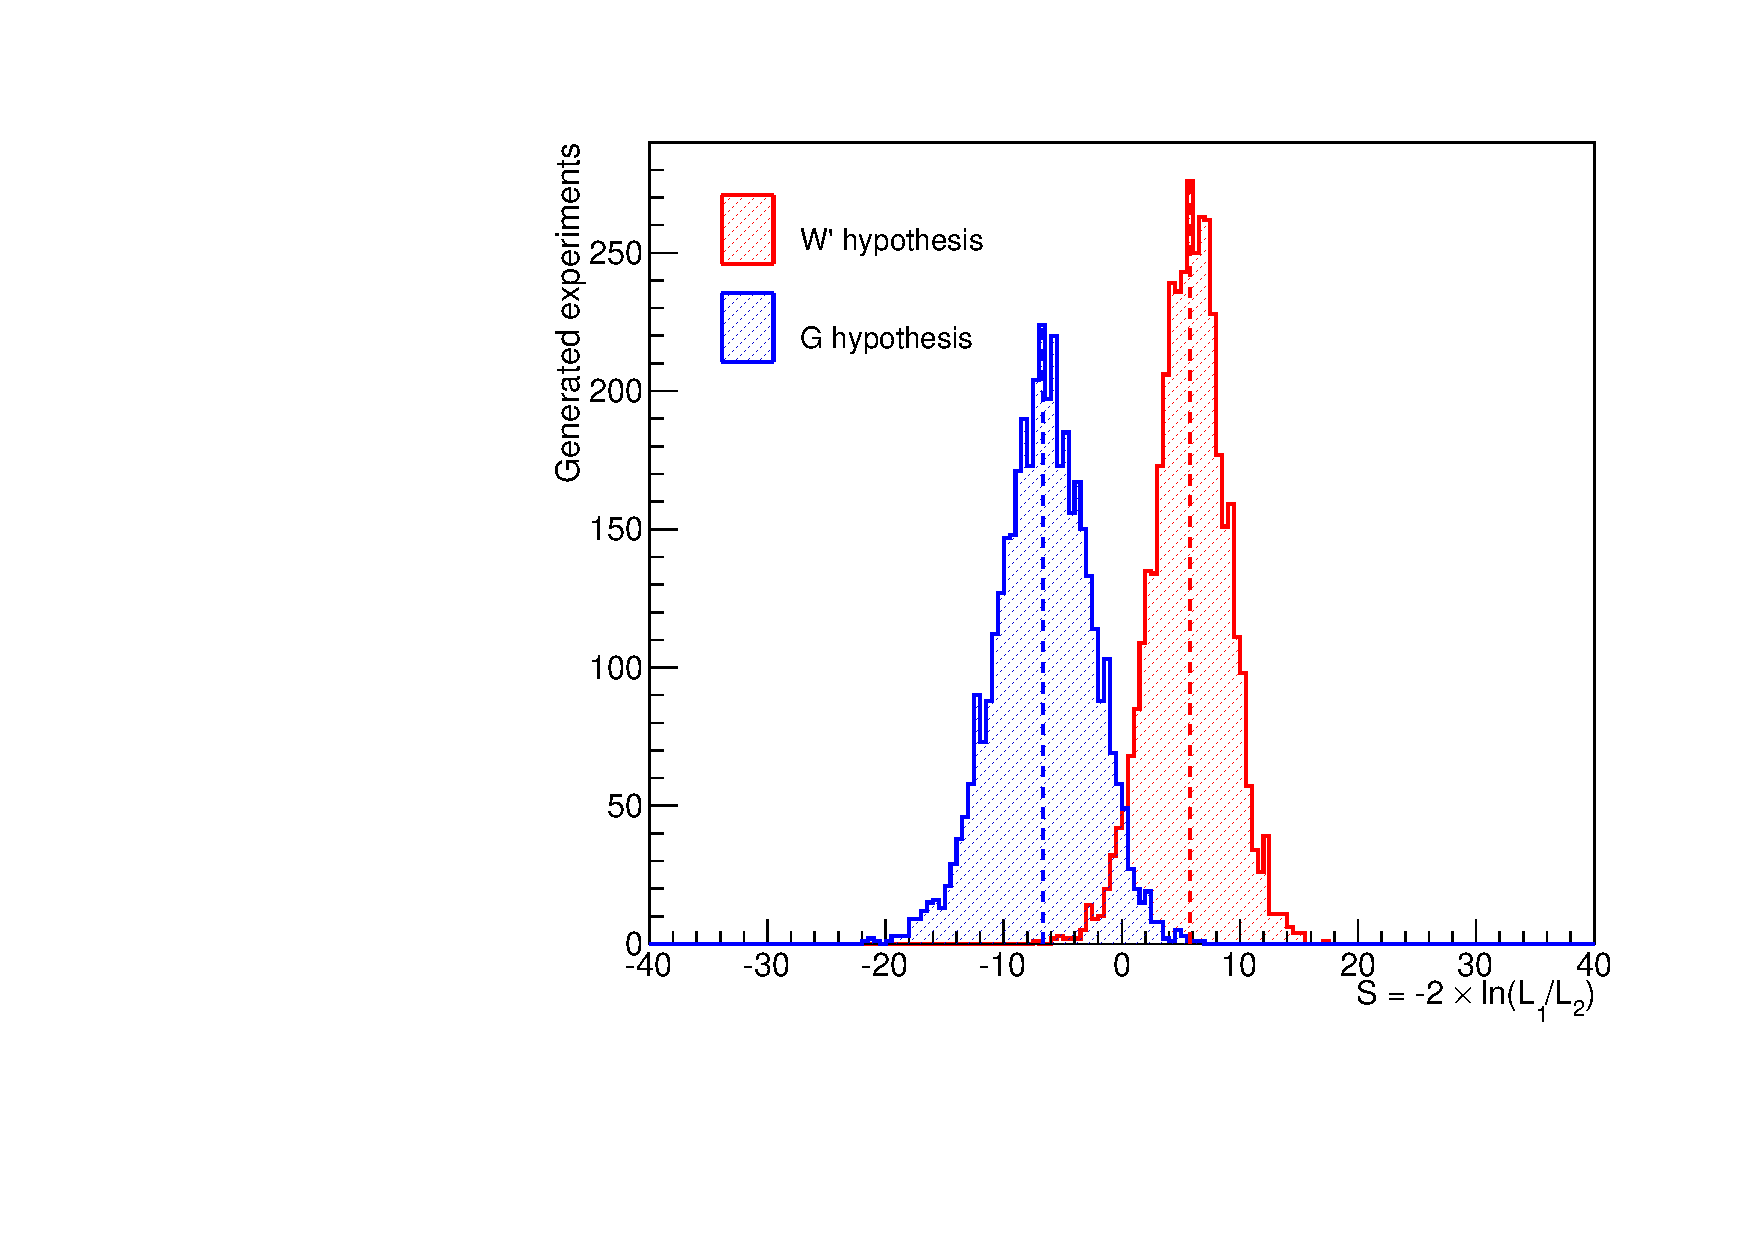
\includegraphics[width=0.49\textwidth]{figures/analysis/search1/AN-15-196/massCategories/sig_sep.pdf}
 \caption{Distribution of the test statistic  $q = -2 \ln(L_{\BulkG}/L_{\PWpr})$ for a \BulkG (blue) and \PWpr signal hypothesis.}
 \label{fig:searchI:signalsep}
 \end{figure}
With the high-purity and low-purity categories as defined above for each mass window combination, this leaves us with six different signal categories:  HP with 3 mass categories corresponding to WW, WZ, and ZZ, and the same 3 mass categories for LP. In parallel to the mass-category based analysis, we perform an analysis without categorization in mass (similar to the 8 \TeV analysis) as a cross-check. We found the sensitivity with mass categories to be higher and hence will not present these studies here. The final tagging efficiency for different signal hypotheses (top) together with the QCD mistag rate (bottom) in the different signal categories is shown in Figure~\ref{fig:search1:sigeff}. The solid lines represent the tagging efficiency in the full mass window ($65 {\GeV} < m_{p} < 105 {\GeV}$) before splitting into mass categories. A lower signal efficiency in the ZZ mass category is observed in all cases. This can be explained from the pruned jet mass distribution on the left in Figure~\ref{fig:wtag}, where a lower pruned jet mass selection of 85 GeV leaves a large fraction of the Z peak in the W mass window. The main benchmark models under consideration preferably decay to W bosons, since in the Bulk Graviton model the branching ratio BR($G_{Bulk}$ $\rightarrow$\WW) = 2* BR($G_{Bulk}$$\rightarrow$ \ZZ) and in the HVT model \PWpr/\PZpr$\rightarrow$ WZ/WW (but not \ZZ). Therefore, the tagging procedure is optimized for a high efficiency to tag W bosons. In the limit-setting procedure all the categories are combined and the overall signal efficiency is maintained. For the combined mass-categories (solid line) the signal efficiency is between 16 and 23\% in the double-tag categories, and between 20 and 34 \% in the single-V tag categories. The mistagging rate is below 1\% in the high-purity category.
\begin{figure}[h!]
\centering
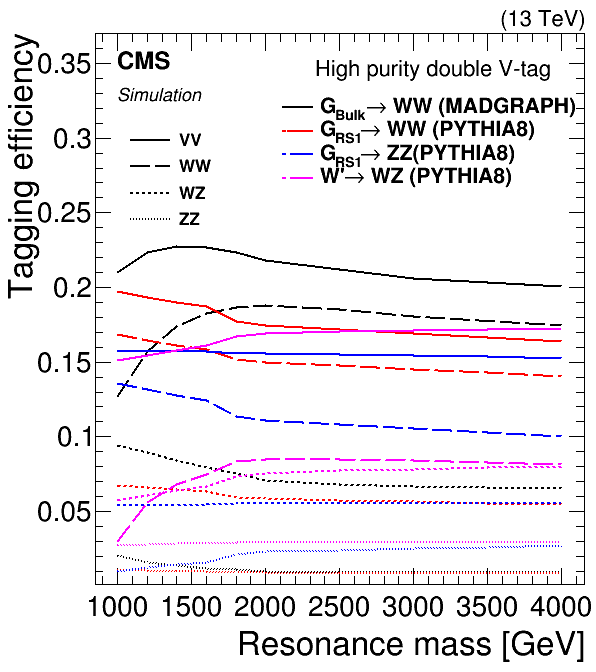
\includegraphics[width=0.4\textwidth]{figures/analysis/search1/AN-15-211/HP_VV_SigEff.png}
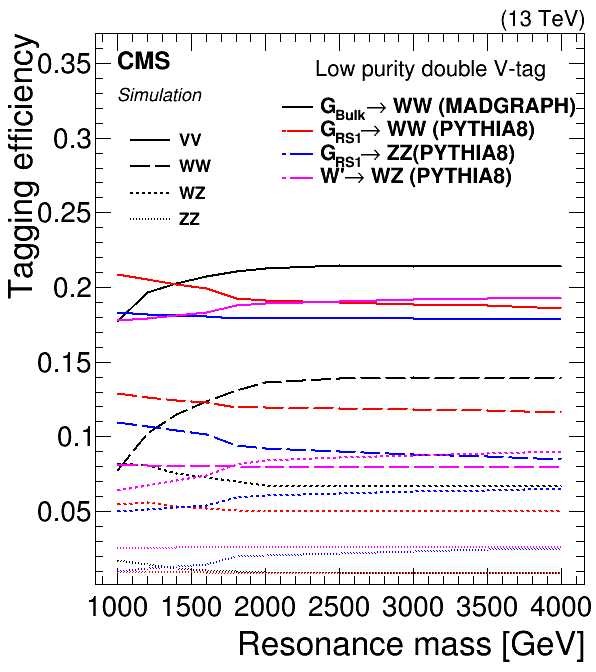
\includegraphics[width=0.4\textwidth]{figures/analysis/search1/AN-15-211/LP_VV_SigEff.png}\\
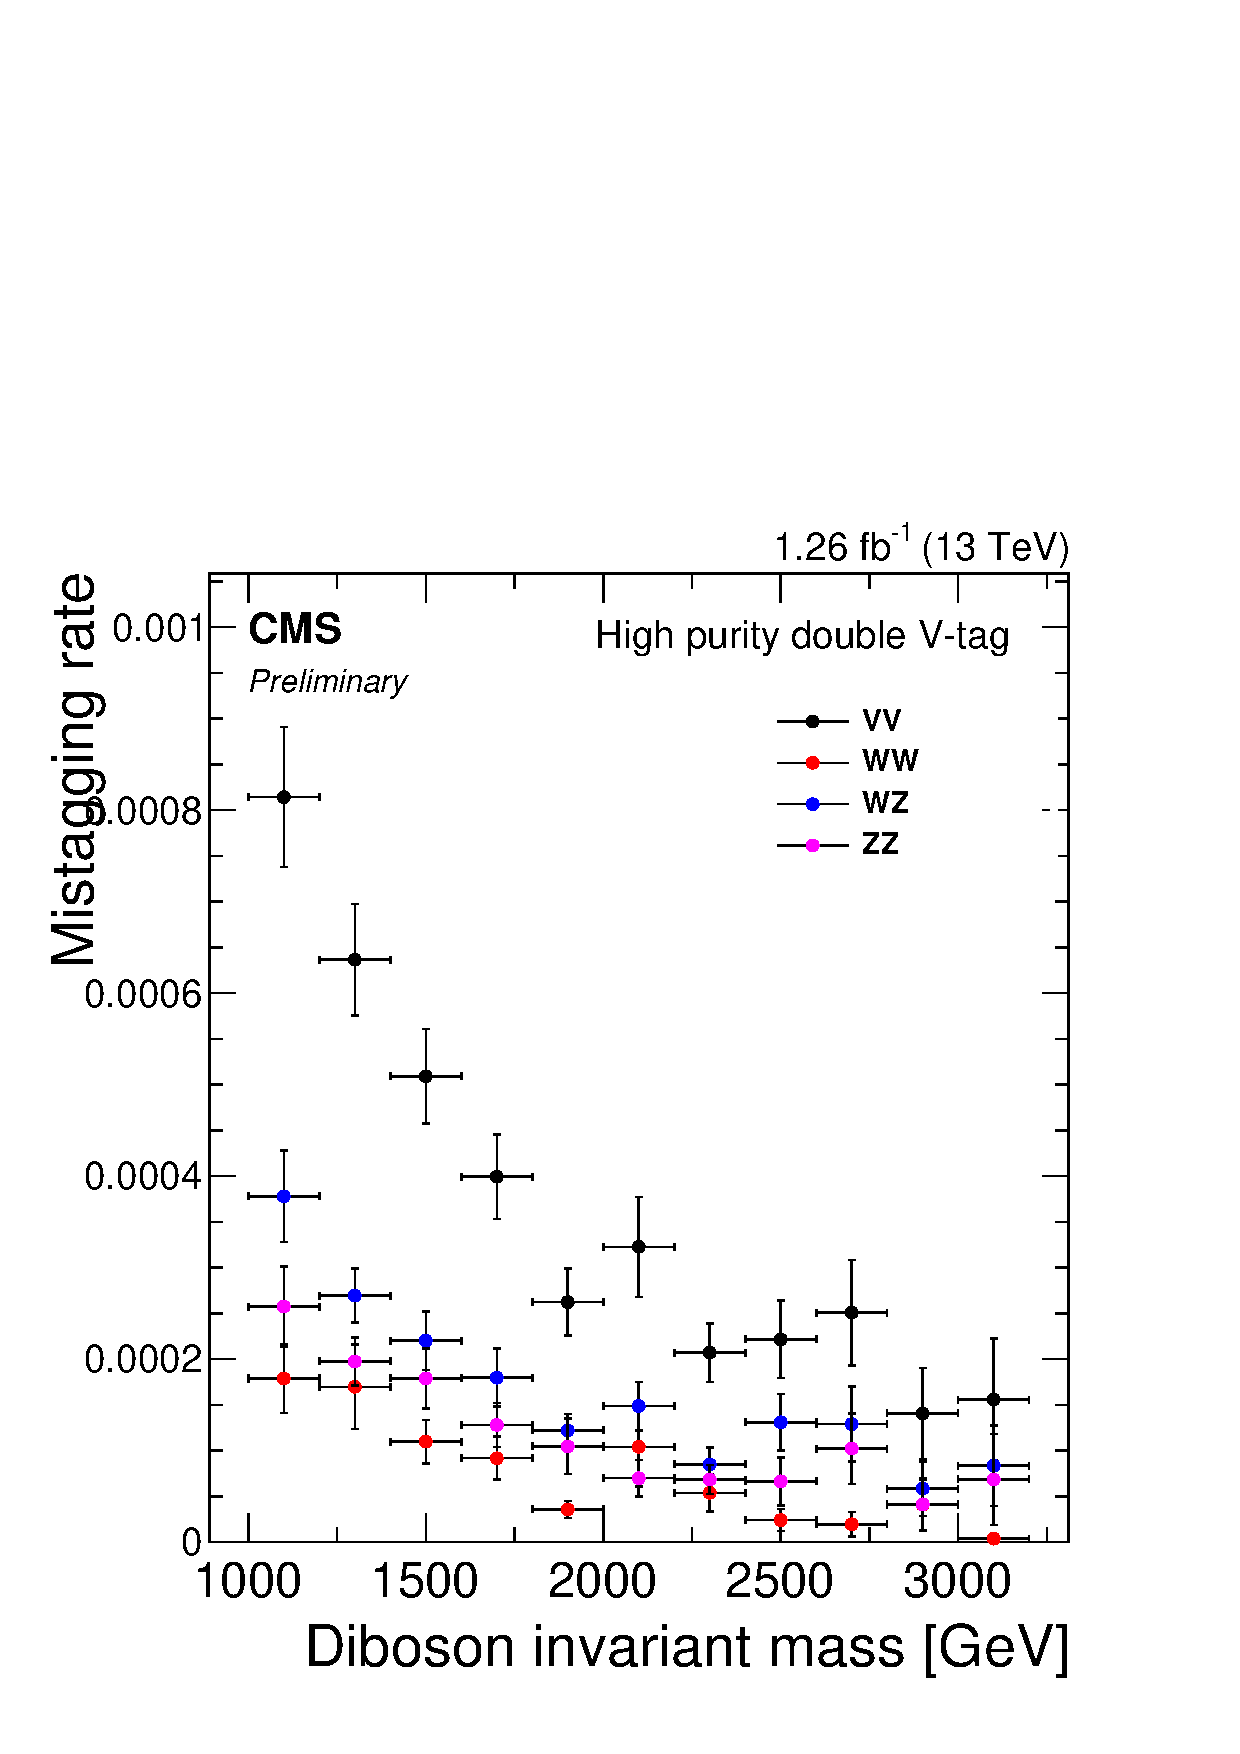
\includegraphics[width=0.4\textwidth]{figures/analysis/search1/AN-15-211/QCD_HP_VV_MistaggingRateEff.pdf}
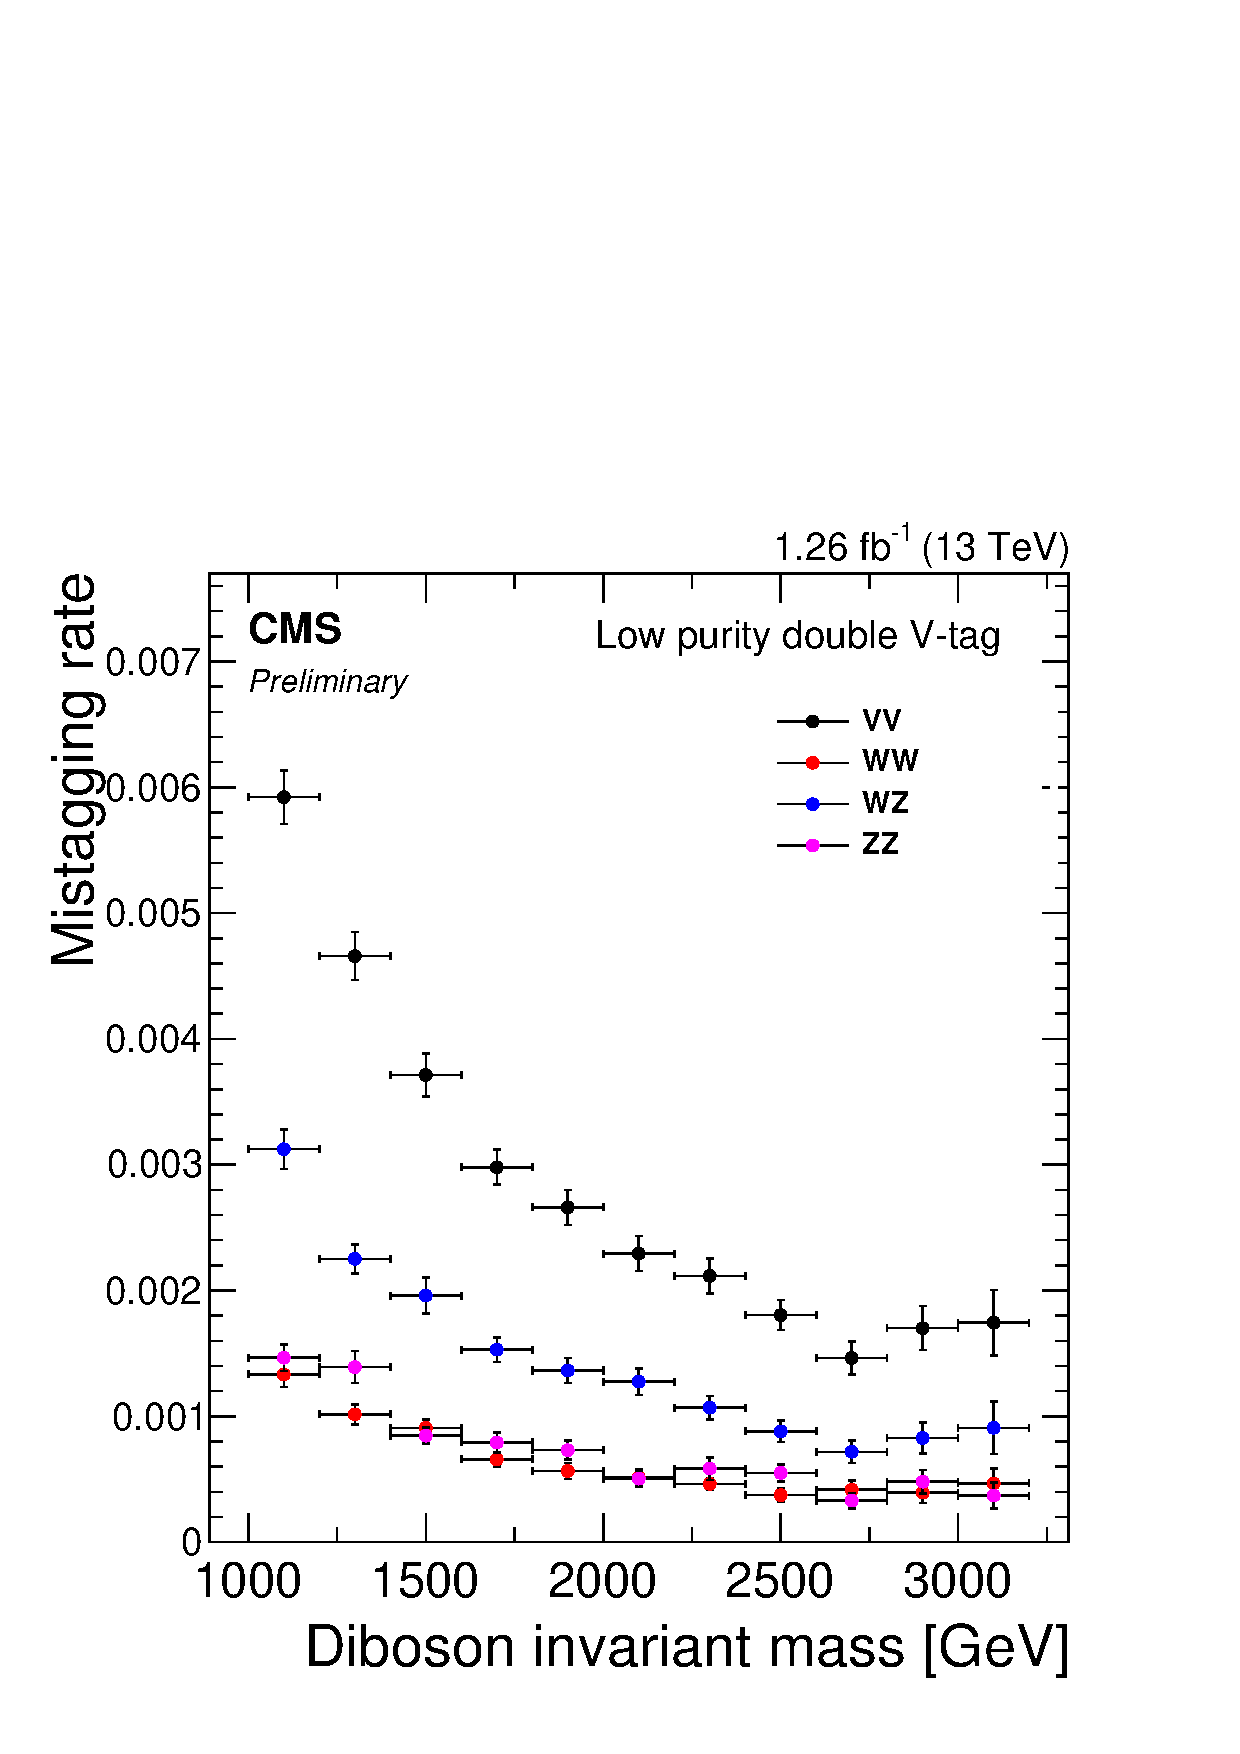
\includegraphics[width=0.4\textwidth]{figures/analysis/search1/AN-15-211/QCD_LP_VV_MistaggingRateEff.pdf}
\caption{Tagging efficiency (top) and mistagging rate (bottom) in the different pruned mass categories in the high-purity category (left) and in the low-purity category (right).}
\label{fig:search1:sigeff}
\end{figure}
The full analysis selections and final signal categories are listed in Table~\ref{tab:search1:selection}, where ${\mJ}_1$ and ${\mJ}_2$ refers to the jet with the highest and second highest jet \PT, respectively.
\begin{table}[!h!]
\footnotesize
\begin{center}
\renewcommand{\arraystretch}{1.2}
\begin{tabular}{lc}
\hline 
\multicolumn{1}{c}{Selection} & Value\\
\hline \hline
\multicolumn{1}{c}{Boson selections}\\
\cline{1-1}
V $\to\qqbar$ (2 AK8 jets) & $\pt >200\GeV$\\
  & $|\eta| < 2.4$\\
Pruned jet mass & $65 < {\mJ}_1,{\mJ}_2  < 105\GeV$\\
Topology    & $|\Delta \eta_\mathrm{jj}| < 1.3$\\
Dijet invariant mass     & $\mjj >1\TeV$\\ 
2- to 1-subjettiness ratio    & $\nsubj < 0.75$\\
\hline
%\hline
\multicolumn{1}{c}{\mJ{} categories}\\
\cline{1-1}
WW & $ 65 < {\mJ}_{1} < 85\GeV$, $ 65 < {\mJ}_{2} < 85\GeV$\\
WZ & $ 65 < {\mJ}_{1} < 85\GeV$, $ 85 < {\mJ}_{2} < 105\GeV$\\
ZZ & $ 85 < {\mJ}_{1} < 105\GeV$, $ 85 < {\mJ}_{2} < 105\GeV$\\
\hline
\multicolumn{1}{c}{\nsubj{} categories}\\
\cline{1-1}
High-purity   & $\tau_{\rm{21, jet1}} < 0.45$, $\tau_{\rm{21, jet2}} < 0.45$\\
Low-purity    & $\tau_{\rm{21, jet1}} < 0.45$, $0.45 < \tau_{\rm{21, jet2}} < 0.75$\\
\hline						       
\end{tabular}
\caption{The full analysis selections, and the signal categories based on the pruned jet mass and \nsubj values.}
\label{tab:search1:selection}
\end{center}
\end{table}
\clearpage

\section{Background modeling}
\label{sec:searchI:bkg}
We assume that the QCD multijets background can be described by a smooth, monotonically decreasing function, which is parametrizable. This is similar to what is done in previous CMS analyses looking for bumps in the dijet invariant mass spectrum~\cite{Chatrchyan:2012ypy,CMS-PAS-EXO-12-059}. The search is then performed by fitting the sum of the functions for background and signal to the dijet invariant mass spectrum in data. Neither data control regions nor simulated samples are used directly by this method. The background functions are of the following form:
\begin{equation}
\label{eq:dijet1}
\frac{dN}{d\mjj}= \frac{ P_0 } { (\mjj/\sqrt{s})^{P_2} }\quad\quad\quad{\rm and}
\quad\quad\quad\quad
\frac{dN}{d\mjj}= \frac{ P_0(1-\mjj/\sqrt{s})^{P_1} } { (\mjj/\sqrt{s})^{P_2} }\:\:,
\end{equation}
where $m$ is the dijet invariant mass, $\sqrt{s}$ is the center-of-mass energy, $P_0$ is a normalization parameter for the probability density function, and $P_1$ and $ P_2$ describe the shape. The number of fit parameters is decided through a Fisher's F-test~\cite{RePEc:bla:istatr:v:80:y:2012:i:3:p:491-491}. In this test, we start from the 2-parameter function and compare the goodness of fit ($\chi^2$ divided by degrees of freedom) when fitting the data signal region with a 2, 3, 4 and 5 parameter function. If the confidence level is less than 10\%, we add additional parameters to model the background distribution. The 4- and 5-parameter functions are
\begin{align}
\label{eq:dijet2}
\frac{dN}{d \mjj} &= \frac{ P_0(1-\mjj/\sqrt{s})^{P_1} } {(\mjj/\sqrt{s})^{P_2+P_3\times\log(\mjj/\sqrt{s})} }\quad{\rm and}\\
\frac{dN}{d \mjj} &= \frac{ P_0(1-\mjj/\sqrt{s})^{P_1} } {(\mjj/\sqrt{s})^{P_2+P_3\times\log(\mjj/\sqrt{s})+P_4\times\log(\mjj/\sqrt{s})^2} },
\end{align}
where $P_3$ and $P_4$ are additional free parameters. As an additional crosscheck, an alternative fit function is also tested:
\begin{equation}
\label{eq:dijet4}
\frac{dN}{d\mjj} = \frac{ P_0(1-\mjj / \sqrt{s}+P_3(\mjj / \sqrt{s})^2)^{P_1} } { (\mjj/\sqrt{s})^{P_2} }.
\end{equation}
The fit range is chosen such that it starts where the trigger efficiency has reached its plateau to avoid bias from trigger inefficiency, and extends to the bin after the highest $m_{VV}$ mass point. The binning chosen for the fit follows the detector resolution as in Refs.~\cite{Chatrchyan:2012ypy,CMS-PAS-EXO-12-059}, and is referred to as the "dijet binning". Before unblinding the signal region, we check that the QCD dijet invariant mass spectrum is expected to be smooth from the distribution in QCD MC as well as exercise the F-test in QCD MC and in a data sideband.\par
The fits to data in the signal region using the different fit functions are shown in Figure \ref{fig:searchI:fit-dataVV}, and the corresponding F-test output are given in Tables~\ref{tab:WW_enriched} through~\ref{tab:ZZ_enriched}. The findings can be summarized as follows: for the WW enriched category, a 2-parameter fit is sufficient to describe the data in both the high- and low-purity categories. In the WZ category, a 2-parameter fit is sufficient in the high-purity category, while three parameters are needed for the low-purity category. For the ZZ category, a 3-parameter fit is needed for both purity categories. The 2- and 3-parameter fit functions as defined in Equation \ref{eq:dijet2} will therefore be used to model the background component in the simultaneous signal and background fit.
\begin{figure}[h!]
\centering
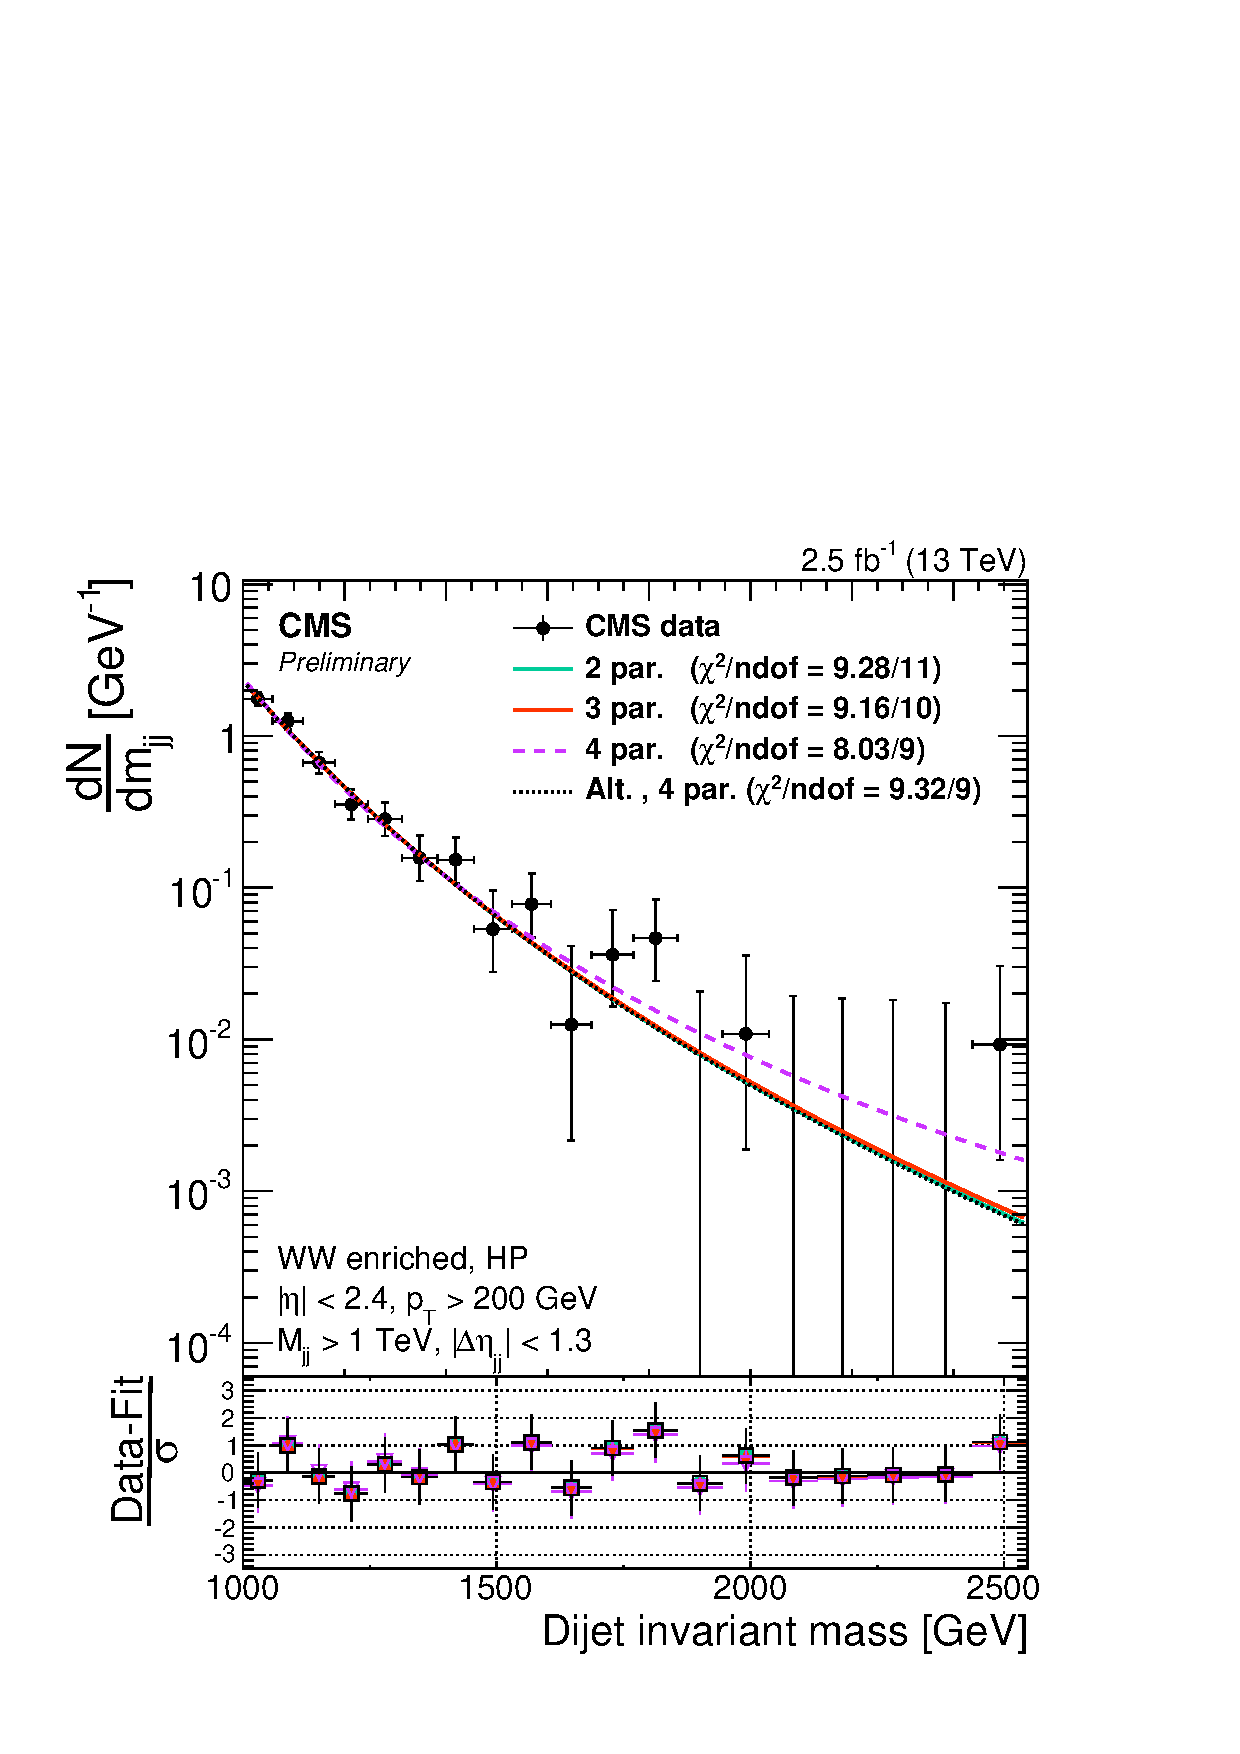
\includegraphics[width=0.32\textwidth]{figures/analysis/search1/AN-15-211/ftest/no5par/WWHP_fitComp.pdf}
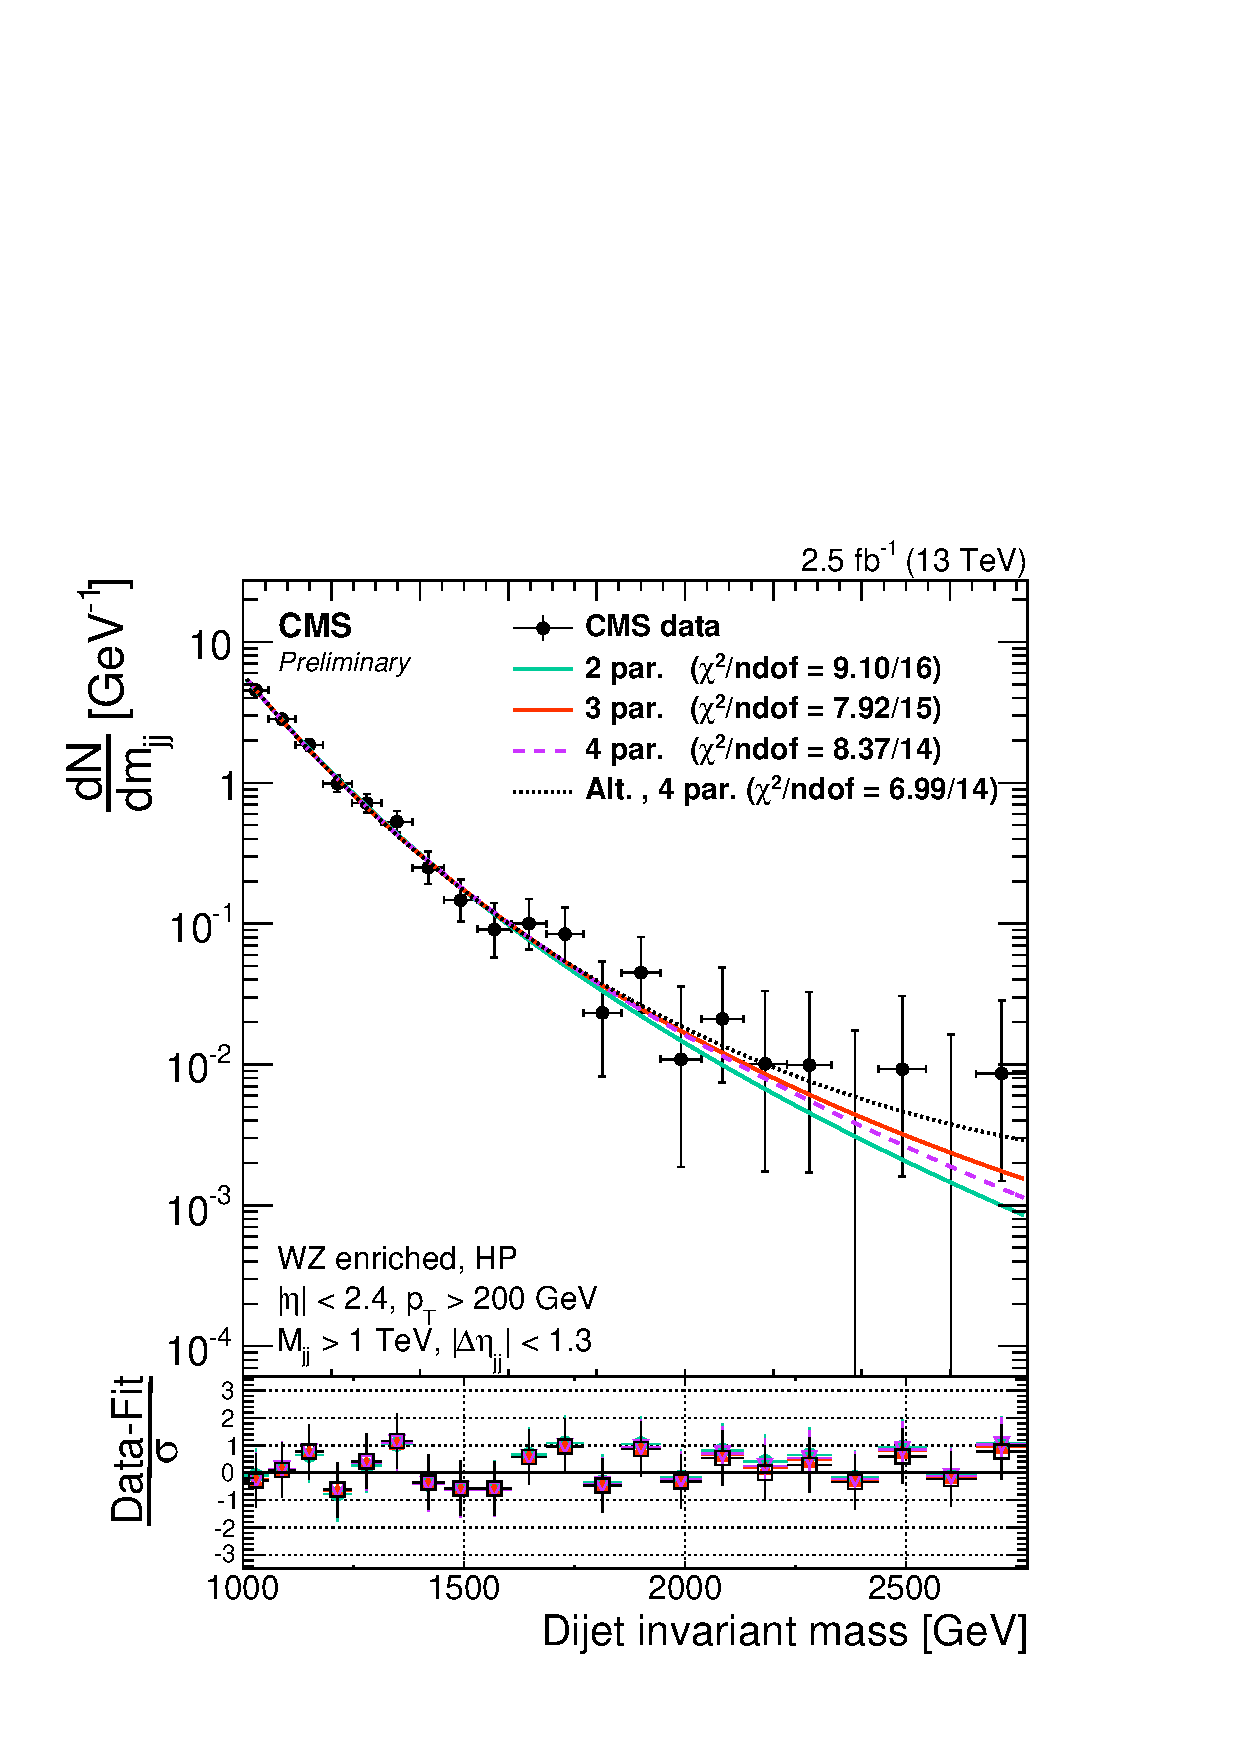
\includegraphics[width=0.32\textwidth]{figures/analysis/search1/AN-15-211/ftest/no5par/WZHP_fitComp.pdf}
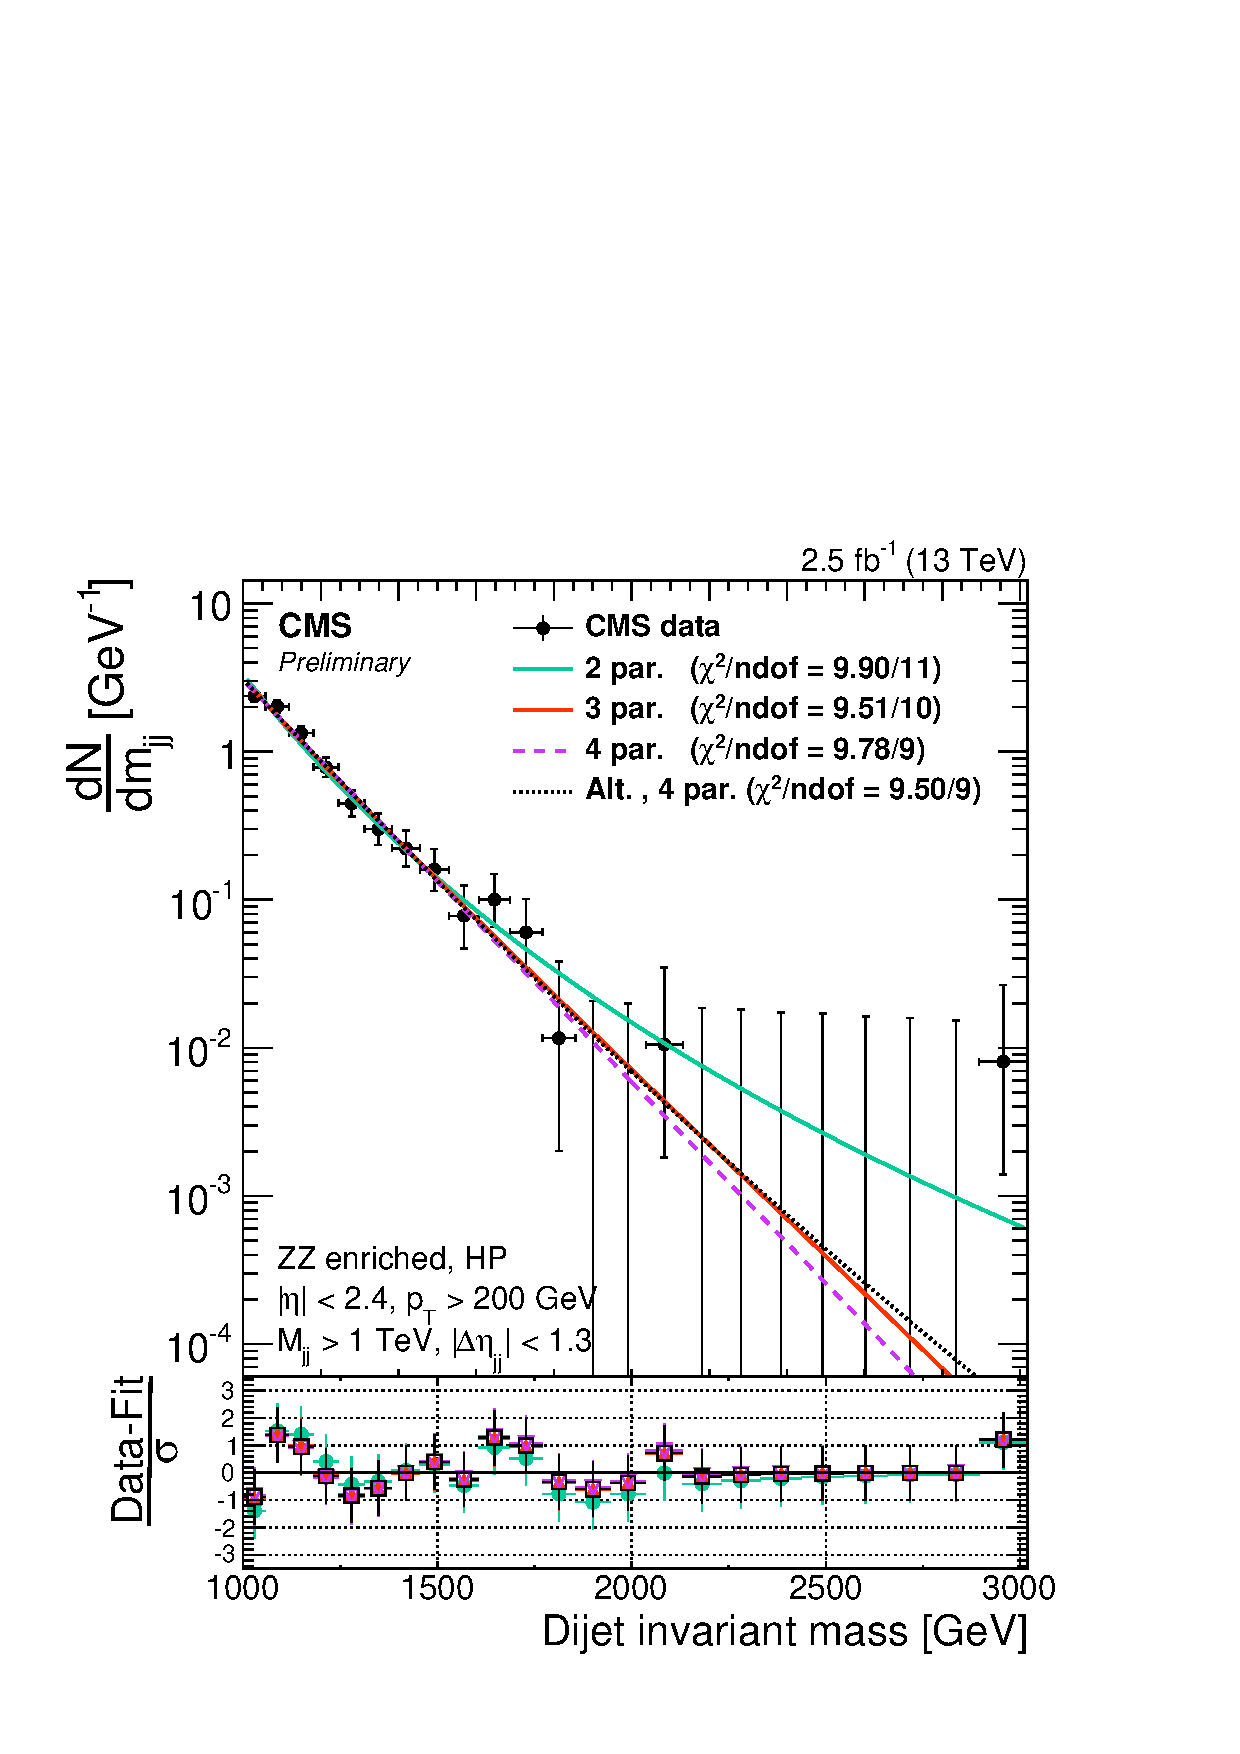
\includegraphics[width=0.32\textwidth]{figures/analysis/search1/AN-15-211/ftest/no5par/ZZHP_fitComp.pdf}\\
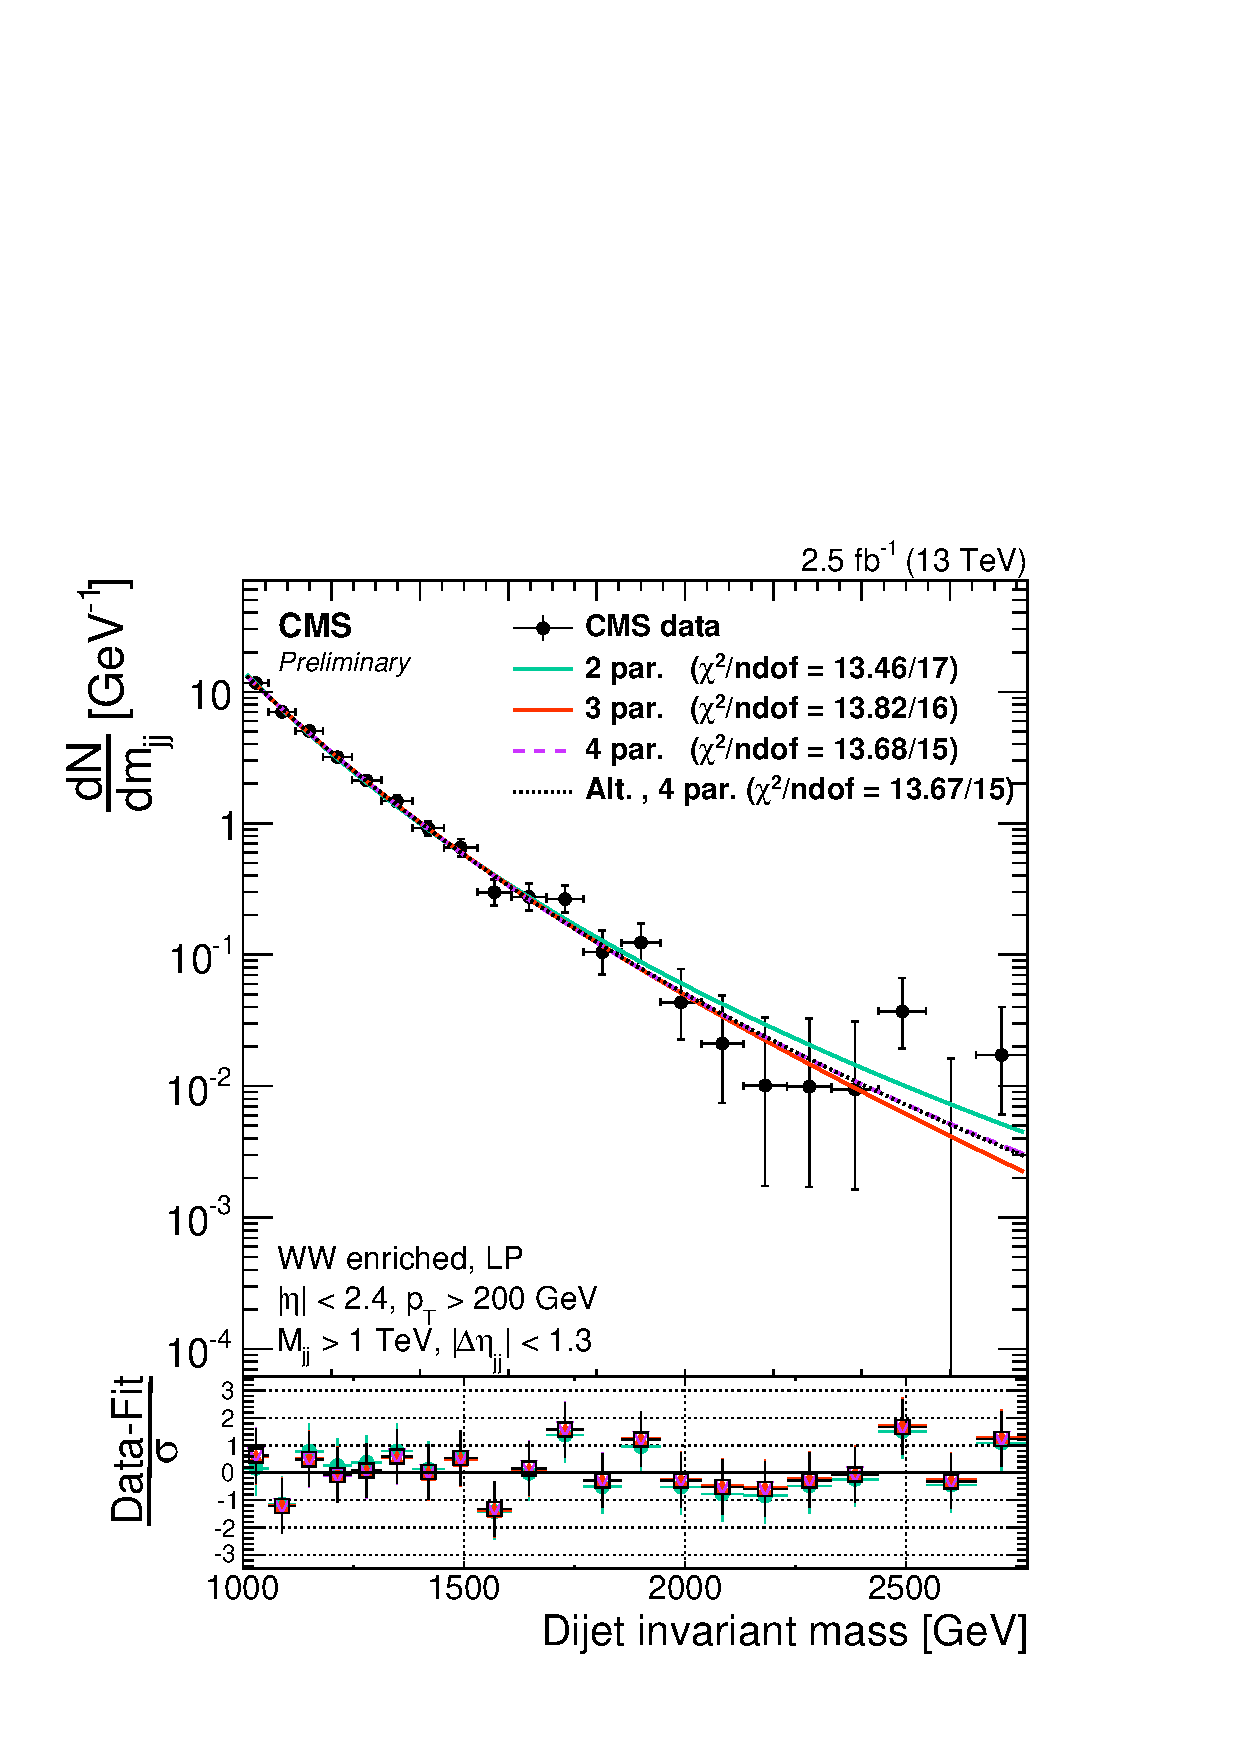
\includegraphics[width=0.32\textwidth]{figures/analysis/search1/AN-15-211/ftest/no5par/WWLP_fitComp.pdf}
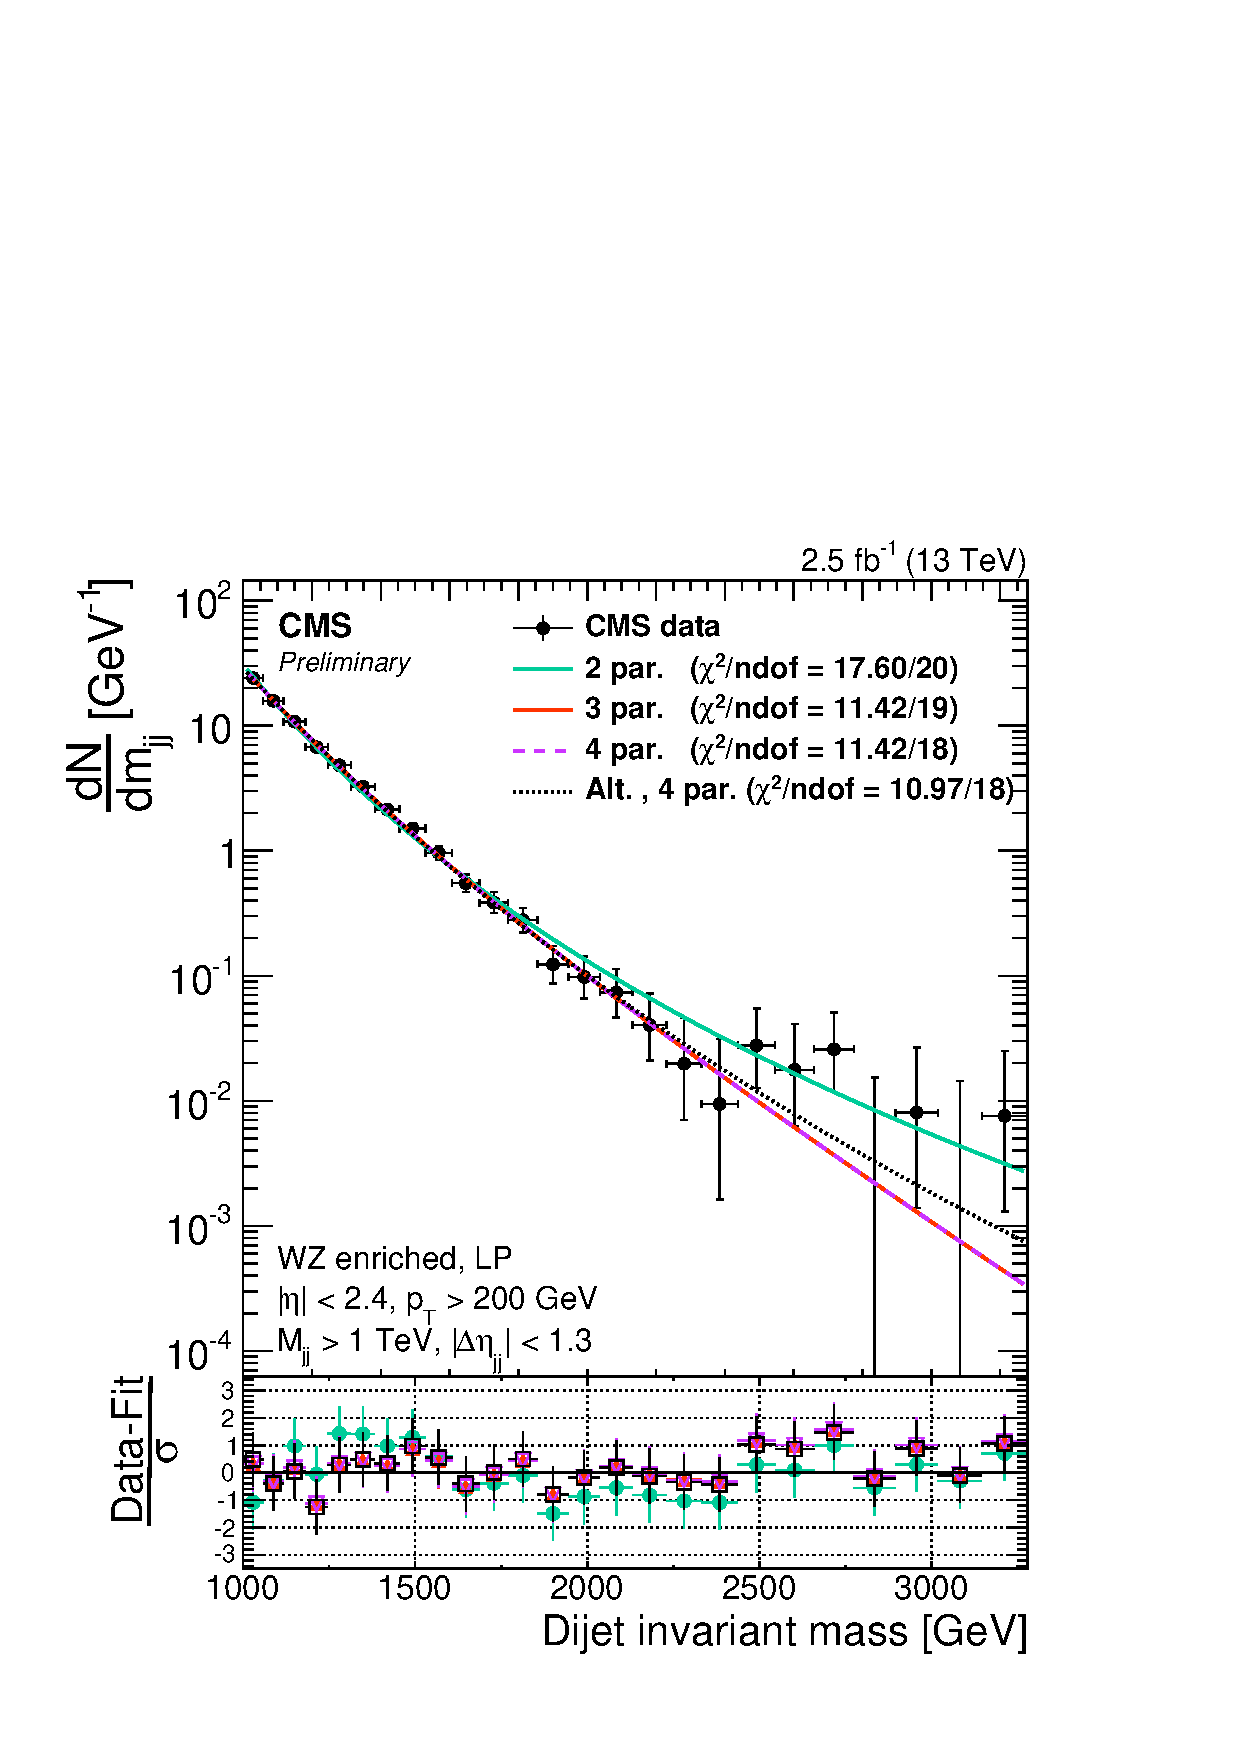
\includegraphics[width=0.32\textwidth]{figures/analysis/search1/AN-15-211/ftest/no5par/WZLP_fitComp.pdf}
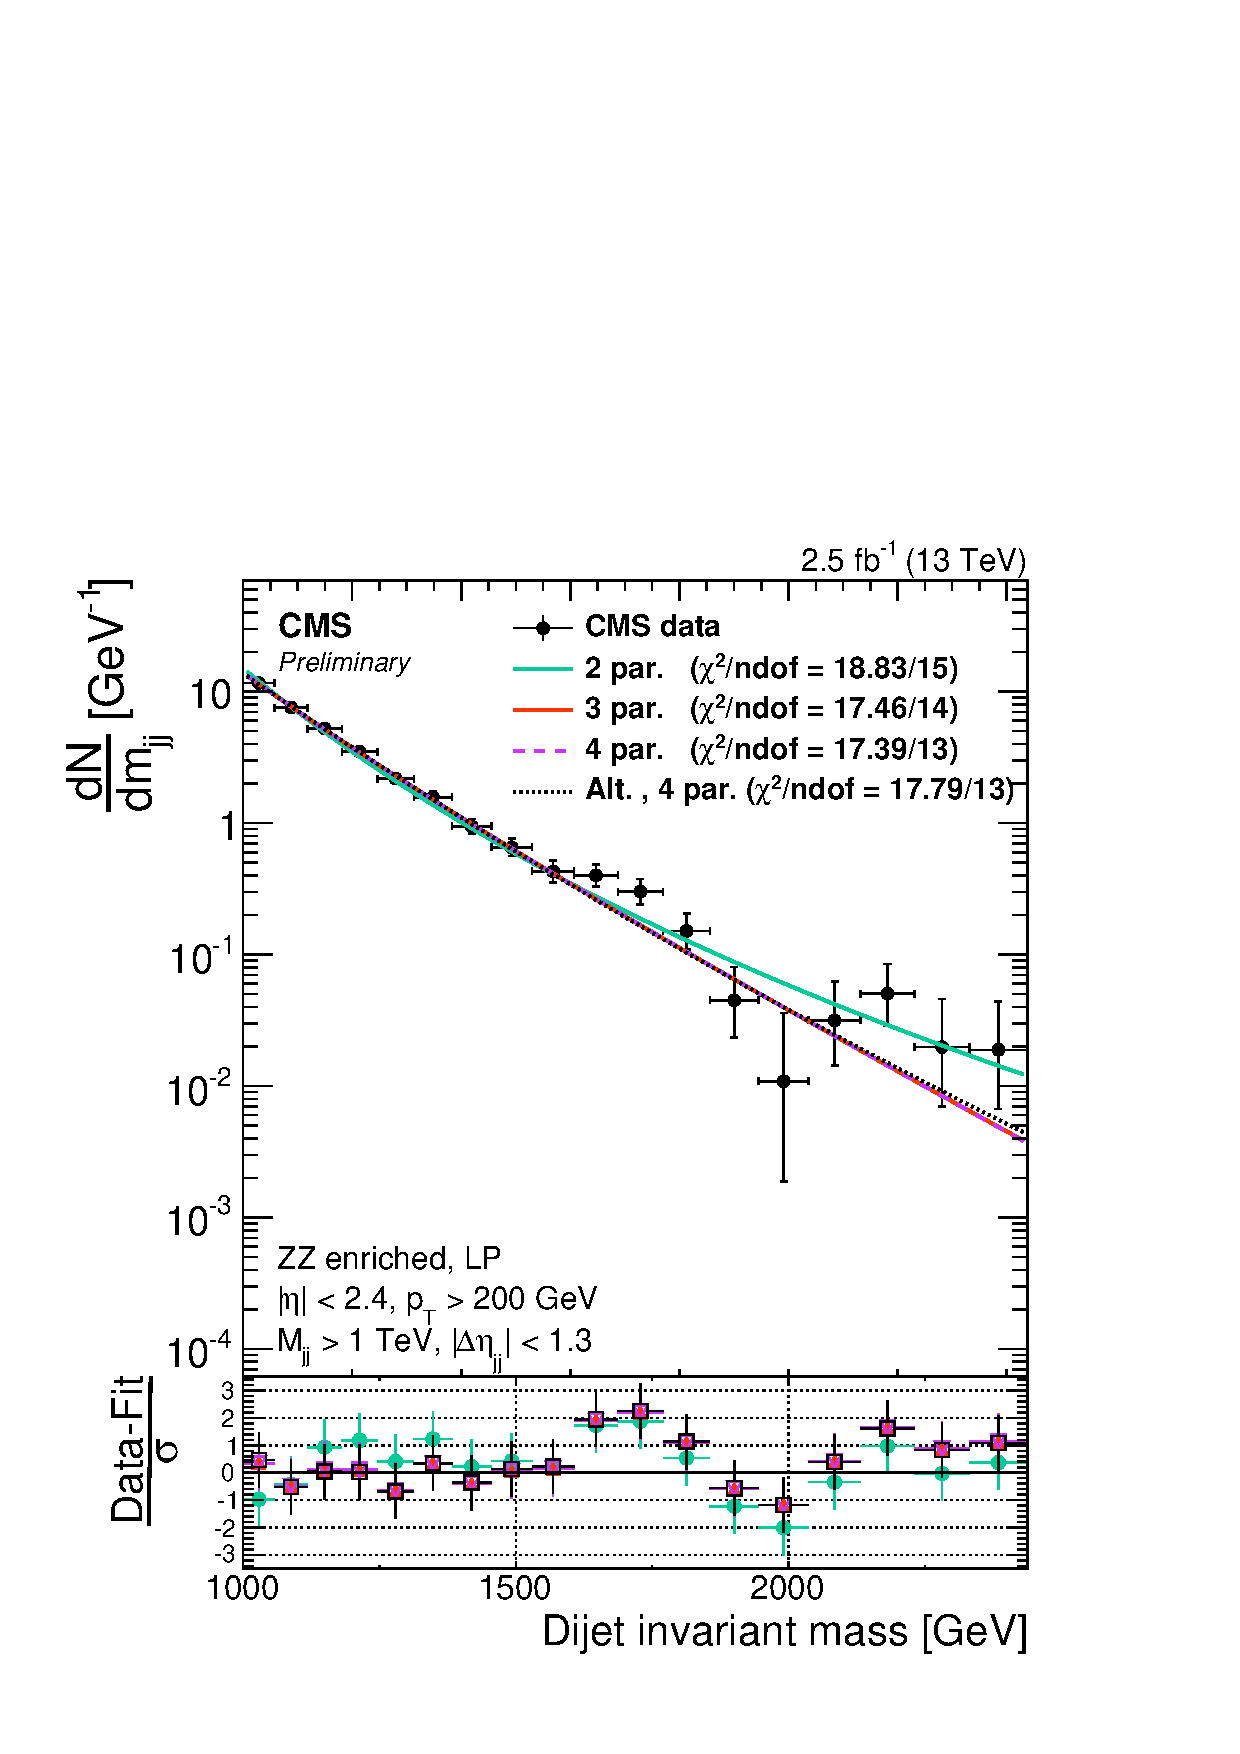
\includegraphics[width=0.32\textwidth]{figures/analysis/search1/AN-15-211/ftest/no5par/ZZLP_fitComp.pdf}
\caption{Fitted dijet mass spectrum in the different mass and purity categories in data. A 2-parameter fit is sufficient to describe the data in the WW- (HP and LP) and WZ-enriched (LP) categories. For the ZZ- (HP and LP) and WZ-enriched (HP) categories, a 3-parameter fit is needed.}
\label{fig:searchI:fit-dataVV}
\end{figure}
\begin{table}[h!]
\centering
\begin{tabular}{|l c c c |}
\hline
\multicolumn{4}{|c|}{WW-enriched, HP}\\
\hline
Function & Residuals & $\chi^2$ & ndof \\
\hline
2 par & 0.034 & 9.279 & 11 \\
3 par & 0.034 & 9.160 & 10 \\
4 par & 0.040 & 8.030 & 9 \\
\hline
\hline
Fishers23  & -0.053 &CL &1.0\\
Fishers34  & -1.456 &CL &1.0\\
\hline
\end{tabular}
\quad
\begin{tabular}{|l c c c |}
\hline
\multicolumn{4}{|c|}{WW-enriched, LP}\\
\hline
Function & Residuals & $\chi^2$ & ndof \\
\hline
2 par & 0.270 & 13.462 & 17 \\
3 par & 0.300 & 13.819 & 16 \\
4 par & 0.324 & 13.680 & 15 \\
\hline
\hline
Fishers23 & -1.723& CL & 1.0\\
Fishers34 & -1.191& CL & 1.0\\
\hline
\end{tabular}
\caption{Residuals, $\chi^{2}$, and degrees of freedom for the WW-enriched HP and LP categories. A 2-parameter fit is needed to describe the data in both categories.}
\label{tab:WW_enriched}
\end{table}
\begin{table}[h!]
\centering
\begin{tabular}{|l c c c |}
\hline
\multicolumn{4}{|c|}{WZ-enriched, HP}\\
\hline
Function & Residuals & $\chi^2$ & ndof \\
\hline
2 par & 0.039 & 9.105 & 16 \\
3 par & 0.047 & 7.915 & 15 \\
4 par & 0.048 & 8.370 & 14 \\
\hline
\hline
Fishers23 & -2.598& CL & 1.0\\
Fishers34 & -0.491& CL & 1.0\\
\hline
\end{tabular}
\quad
\begin{tabular}{|l c c c |}
\hline
\multicolumn{4}{|c|}{WZ-enriched, LP}\\
\hline
Function & Residuals & $\chi^2$ & ndof \\
\hline
2 par & 1.016 & 17.602 & 20 \\
3 par & 0.270 & 11.424 & 19 \\
4 par & 0.269 & 11.421 & 18 \\
\hline
\hline
Fishers23 & 55.258& CL & 0.0\\
Fishers34 & 0.078& CL & 0.783\\
\hline
\end{tabular}
\caption{Residuals, $\chi^{2}$, and degrees of freedom for the WZ-enriched HP (left) and LP (right) categories. A 2-parameter fit is sufficient to describe the data in the high-purity category, while three parameters are needed for the low-purity category.}
\label{tab:WZ_enriched}
\end{table}
\begin{table}[h!]
\centering
\begin{tabular}{|l c c c |}
\hline
\multicolumn{4}{|c|}{ZZ-enriched, HP}\\
\hline
Function & Residuals & $\chi^2$ & ndof \\
\hline
2 par & 0.220 & 9.901 & 11 \\
3 par & 0.140 & 9.511 & 10 \\
4 par & 0.124 & 9.781 & 9 \\
\hline
\hline
Fishers23 & 6.302& CL & 0.029\\
Fishers34 & 1.246& CL & 0.290\\
\hline
\end{tabular}
\quad
\begin{tabular}{|l c c c |}
\hline
\multicolumn{4}{|c|}{ZZ-enriched, LP}\\
\hline
Function & Residuals & $\chi^2$ & ndof \\
\hline
2 par & 0.448 & 18.832 & 15 \\
3 par & 0.121 & 17.463 & 14 \\
4 par & 0.118 & 17.394 & 13 \\
\hline
\hline
Fishers23 & 40.438& CL & 0.0\\
Fishers34 & 0.356& CL & 0.56\\
\hline
\end{tabular}
\caption{Residuals, $\chi^{2}$, and degrees of freedom for the ZZ-enriched LP and HP categories. A 3-parameter fit is sufficient to describe the data in both categories.}
\label{tab:ZZ_enriched}
\end{table}

\clearpage
\section{Signal modeling}
\label{sec:searchI:sig}

The signal shape is extracted from signal MC with resonance masses in the range from 1 to 4 TeV. A linear interpolation provides shapes for the mass points in between in steps of 100 GeV. From these shapes, signal shape models are constructed as composite models with a Gaussian core due to detector resolution and an exponential tail to account for parton distribution function effects. Parametric shape uncertainties due to jet energy scale and resolution uncertainties are inserted by variations of the Gaussian peak position and width. The dijet invariant mass shape for different benchmark model signals is shown in Figure \ref{fig:searchI:sigfit}. The signal and background components are then simultaneously fitted to the data points.
\begin{figure}[h!]
\centering
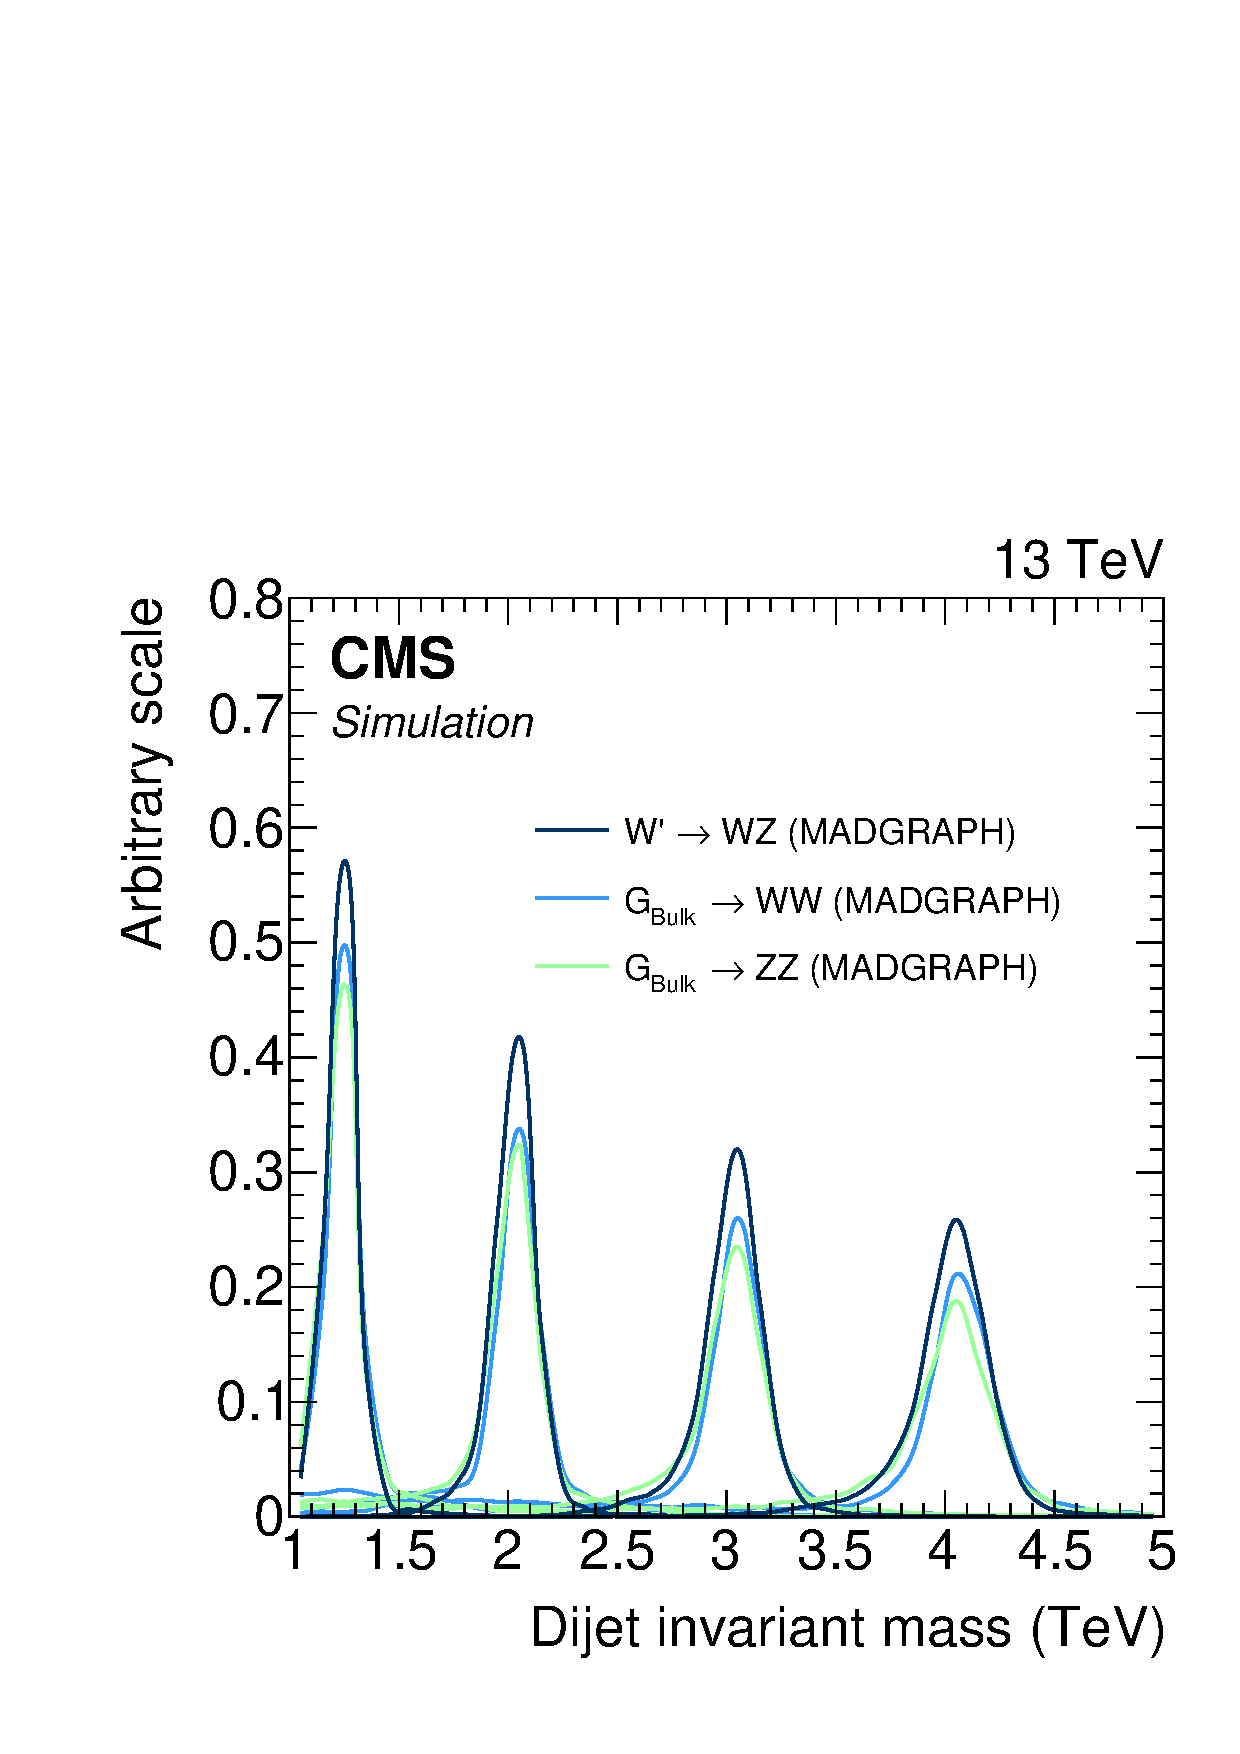
\includegraphics[width=0.49\textwidth]{figures/analysis/search1/B2G-16-004/Figure_005-a.pdf}
\caption{Dijet invariant mass from signal MC used to extract the signal shape, shown here for resonances with masses of 1.2, 2, 3, and 4 TeV.}
\label{fig:searchI:sigfit}
\end{figure}
\clearpage

\section{V-tagging scale factors}
\label{sec:searchI:vtag}
As seen in Figure~\ref{fig:wtag}, a discrepancy is observed in the \nsubj distribution between data and MC. This could lead to a bias in the signal efficiency estimation so we must measure the real signal efficiency in data in an orthogonal data sample.
The W-tagging efficiency is measured using real boosted W-jets in a data sample enriched in \ttbar decays with a hadronically decaying $W$ boson. This region is mainly quark-enriched, as opposed to the gluon-enriched QCD region previously studied, and substructure variables are better described here. The sample is obtained by requiring a final state compatible with two b-jets and two \PW bosons, where one of the bosons decays leptonically and the other one hadronically. There are several good reasons to use this channel: Top-quark pair production events are plentifully produced at the LHC; we can ensure a high purity of the sample by requiring a high-energy lepton, b-tag and missing energy requirements; and lastly, we can ensure that the W jets are boosted by requiring the leptonic leg, together with the hadronic W boson candidate, to have high transverse momentum. The final state is illustrated in Figure~\ref{fig:search2:ttsemilep}, with the object of interest being the AK R=0.8 jet containing the two quark daughters of the hadronically decaying W boson.
\begin{figure}[h!]
\centering
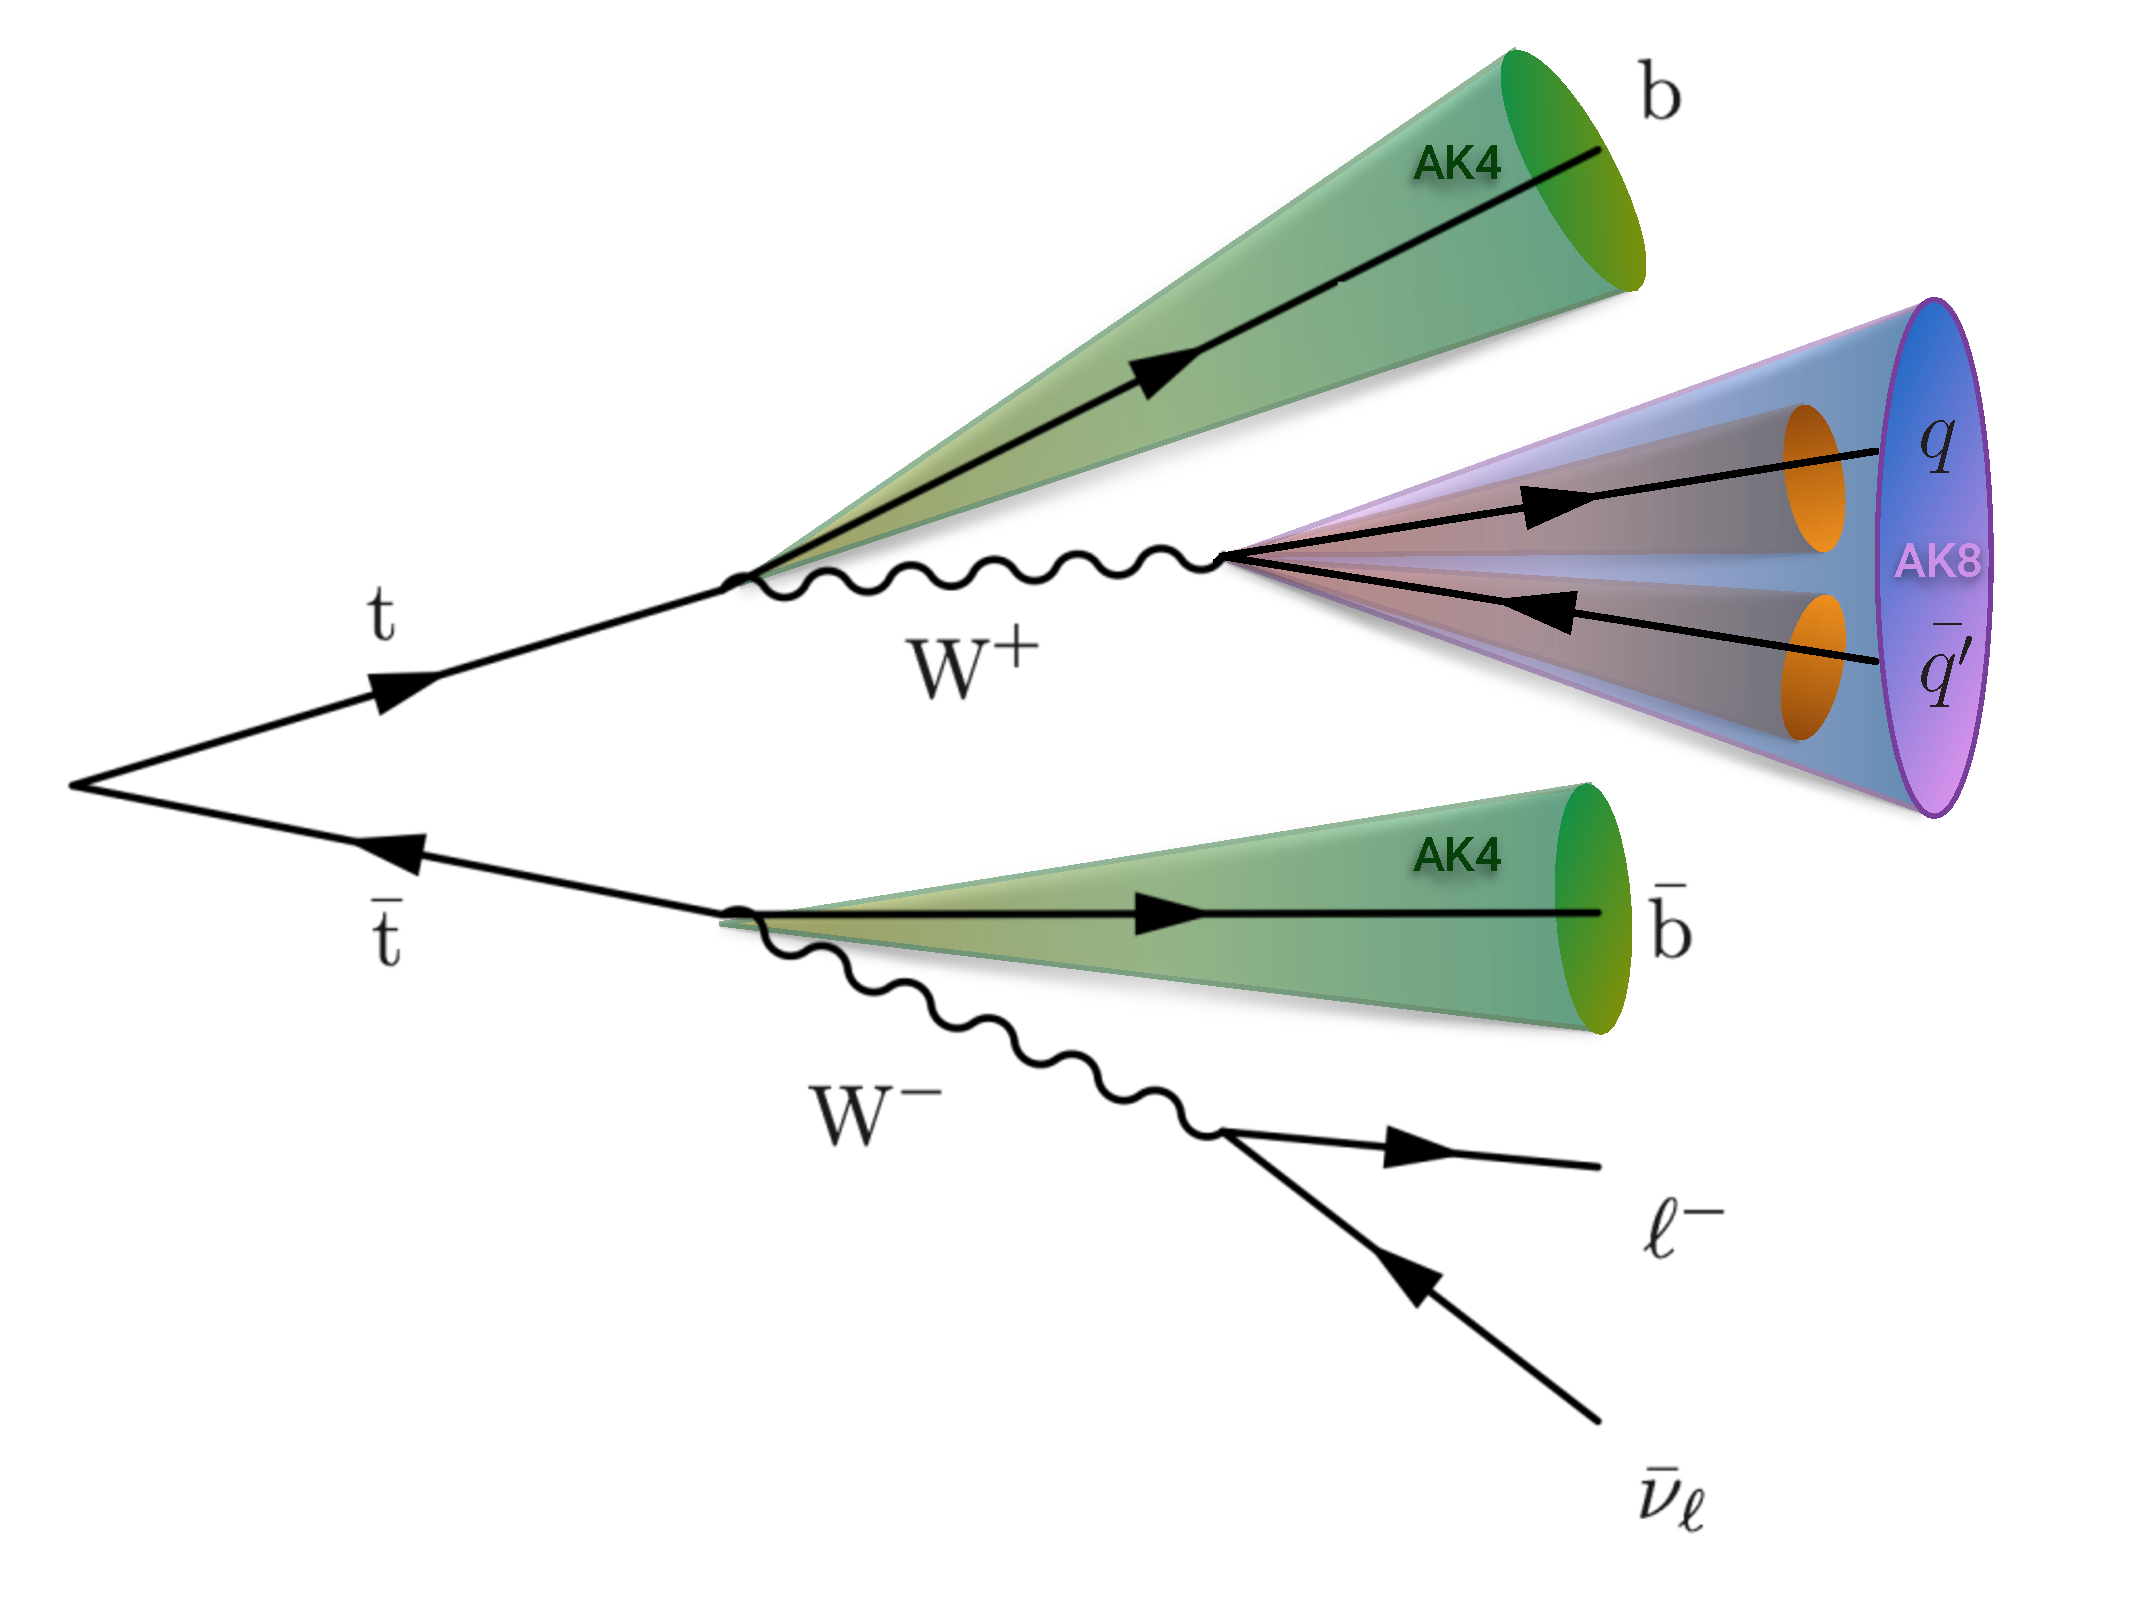
\includegraphics[width=0.49\textwidth]{figures/analysis/search2/misc/semileptt.pdf}
\caption{A top quark pair decaying into two b quarks and two \PW bosons, one of which decays leptonically and one of which decays hadronically.}
\label{fig:search2:ttsemilep}
\end{figure}

\subsection{Event selection}
\label{sec:searchI:vtag:evsel}
The W boson can decay to a neutrino and either an electron or muon, and both final states ("channels") are used in the analysis. We select events by triggering and event selection on the leptonic W decay. First, we require a high-energy lepton at trigger level, with an online \PT above 45 \GeV for the muon or 135 \GeV for the electron. This requires an offline muon (electron) \PT threshold of 53 (120) \GeV. The leptons are further required to pass the lepton requirements defined in Section~\ref{sec:objreco:muons}, and events containing additional leptons (passing the same ID requirements, but looser cuts as defined in Table~\ref{tab:searchII:cutsummary}) are vetoed. Offline, we further require a high missing energy of 40 (80) \GeV in the muon(electron) channel. To ensure a high signal purity of boosted, hadronically decaying W bosons, the four-vector of the leptonically decaying W boson is reconstructed such that we can put tight momentum requirements on the leptonic W boson (ensuring that both tops, and therefore vector bosons, have a high momentum). The leptonic W boson is reconstructed in two steps: First, the unknown z component of the neutrino momentum must be solved for through a second order equation assuming the real W boson mass
\begin{equation*}
M_\mathrm{W}^2 = m_\ell^2   + 2(E_\ell E_\nu - p_{x_\ell}p_{x_\nu} - p_{y_\ell}p_{y_\nu} - p_{z_\ell}p_{z_\nu} ) = (80.4)^2.  
\end{equation*}
This results in a completely defined neutrino four-vector, which is then added to the lepton four-vector. The sum of the two defines the leptonic W boson four-momentum, and its momentum is required to be greater than 200 \GeV. Further, we require at least one AK R=0.4 jet to be b-tagged with the Combined Secondary Vertex (CSV) algorithm~\cite{1748-0221-8-04-P04013,1748-0221-13-05-P05011}. This algorithm exploits the relatively long lifetime and large mass of b hadrons that leads to the presence of a displaced vertex in order to distinguish between jets originating from b quarks and those originating from light-flavor quarks. More information on the CSV algorithm can be found in ~\cite{1748-0221-8-04-P04013,1748-0221-13-05-P05011}. The reason for requiring only one b-tagged jet is to ensure a high selection efficiency. Finally, we require at least one AK R=0.8 jet in the event with a momentum greater than 200 GeV, which will be the hadronic W boson candidate. It's pruned jet mass is required to be between 40 \GeV and 150 \GeV. After reconstructing and selecting all our objects, a set of angular selections are applied to ensure a diboson-like topology. These are the following:
\begin{itemize}
\itemsep0em 
  \item the $\Delta R$ between the lepton and the hadronic W boson candidate must be $< \pi/2$, %$\Delta R(\l,W_{AK8}) > \pi/2$
  \item the $\Delta \phi$ between the hadronic W boson candidate and the $\ETmiss$ must be $>2$, and %$\Delta \phi(W_{AK8},\ETmiss) > 2$
  \item the $\Delta \phi$ between the hadronic W boson candidate and the lepton must be $>2$.%$\Delta \phi(W_{AK8},W_{lep}) > 2$
\end{itemize}
With these requirements, we have a nearly pure sample of \ttbar events, with a small contamination from
from single top-quark production, W+jets, and VV events. A summary of the final selection criteria is presented in Table~\ref{tab:searchII:cutsummary}. The pruned jet mass and \nsubj variables in data and in MC are shown in Figure~\ref{fig:searchI:ttbarcp}.
\begin{table}[h!]
\footnotesize
\centering
\begin{tabular}{lcc}
\hline 
\multicolumn{1}{c}{\textbf{Selection}} & \textbf{Value} & \textbf{Comments}\\
\hline
\multicolumn{1}{c}{\texttt{Tight} Lepton selection}\\
\cline{1-1}
Electron $\PT$ & $\PT > 120 \GeV$    & \\
Muon $\PT$ & $\PT > 53 \GeV$ & \\
Electron $\eta$ & $|\eta|_{\text{SC}} <2.5$ except [1.4442, 1.566] & Veto ECAL barrel-endcap transition.\\
Muon $\eta$  & $|\eta|<2.1$  & \\
\hline
\multicolumn{1}{c}{\texttt{Loose} Lepton selection}\\
\cline{1-1}
Electron $\PT$ & $\PT > 35 \GeV$    & \\
Muon $\PT$ & $\PT > 20 \GeV$ & \\
Electron $\eta$ & $|\eta|_{\text{SC}} <2.5$ except [1.4442, 1.566] & Veto ECAL barrel-endcap transition.\\
Muon $\eta$  & $|\eta|<2.4$  & \\
\hline
\multicolumn{1}{c}{AK8 jet selections}\\
\cline{1-1}
Jet $\PT$ &  $\PT >200~\GeV$ & For hadronic \\
Jet $\eta$  & $|\eta|<2.4$ & W reconstruction \\
\hline
\multicolumn{1}{c}{AK4 jet selections}\\
\cline{1-1}
Jet $\PT$ &  $\PT >30~\GeV$ & Used for b-tag \\
Jet $\eta$  & $|\eta|<2.4$ & jet selection\\
\hline
\multicolumn{1}{c}{\ETmiss selections}\\
\cline{1-1}
\ETmiss (electron channel) &  \ETmiss$>80~\GeV$ & \\
\ETmiss (muon channel) & \ETmiss$>40~\GeV$ & \\
\hline
\multicolumn{1}{c}{Boson selections}\\
\cline{1-1}
Pruned jet mass & $ 40 < m_{p} < 150 \GeV$ &  \\
Leptonic W $\PT$      &  $\PT > 200 \GeV$     & \\
Hadronic W $\PT$      &  $\PT > 200 \GeV$     & \\
\hline
\multicolumn{1}{c}{Veto}\\
\cline{1-1}
Number of \texttt{loose} electrons & 0    &  \\
Number of \texttt{loose} muons & 0    & \\
Number of b-tagged jets           & $>0$    & CSV medium working point \\
\hline
\multicolumn{1}{c}{Angular selections}\\
\cline{1-1}
$\Delta R(\l,W_{AK8})         $ & $> \pi/2$ & \\
$\Delta \phi(W_{AK8},\ETmiss) $ & $> 2$     & \\
$\Delta \phi(W_{AK8},W_{lep}) $ & $> 2$     & \\
\hline
\end{tabular}
\caption{Summary of the final semi-leptonic t$\bar{t}$ selections.}
\label{tab:searchII:cutsummary}
\end{table}

\begin{figure}[ht!]
\centering
\begin{tabular}{cc}
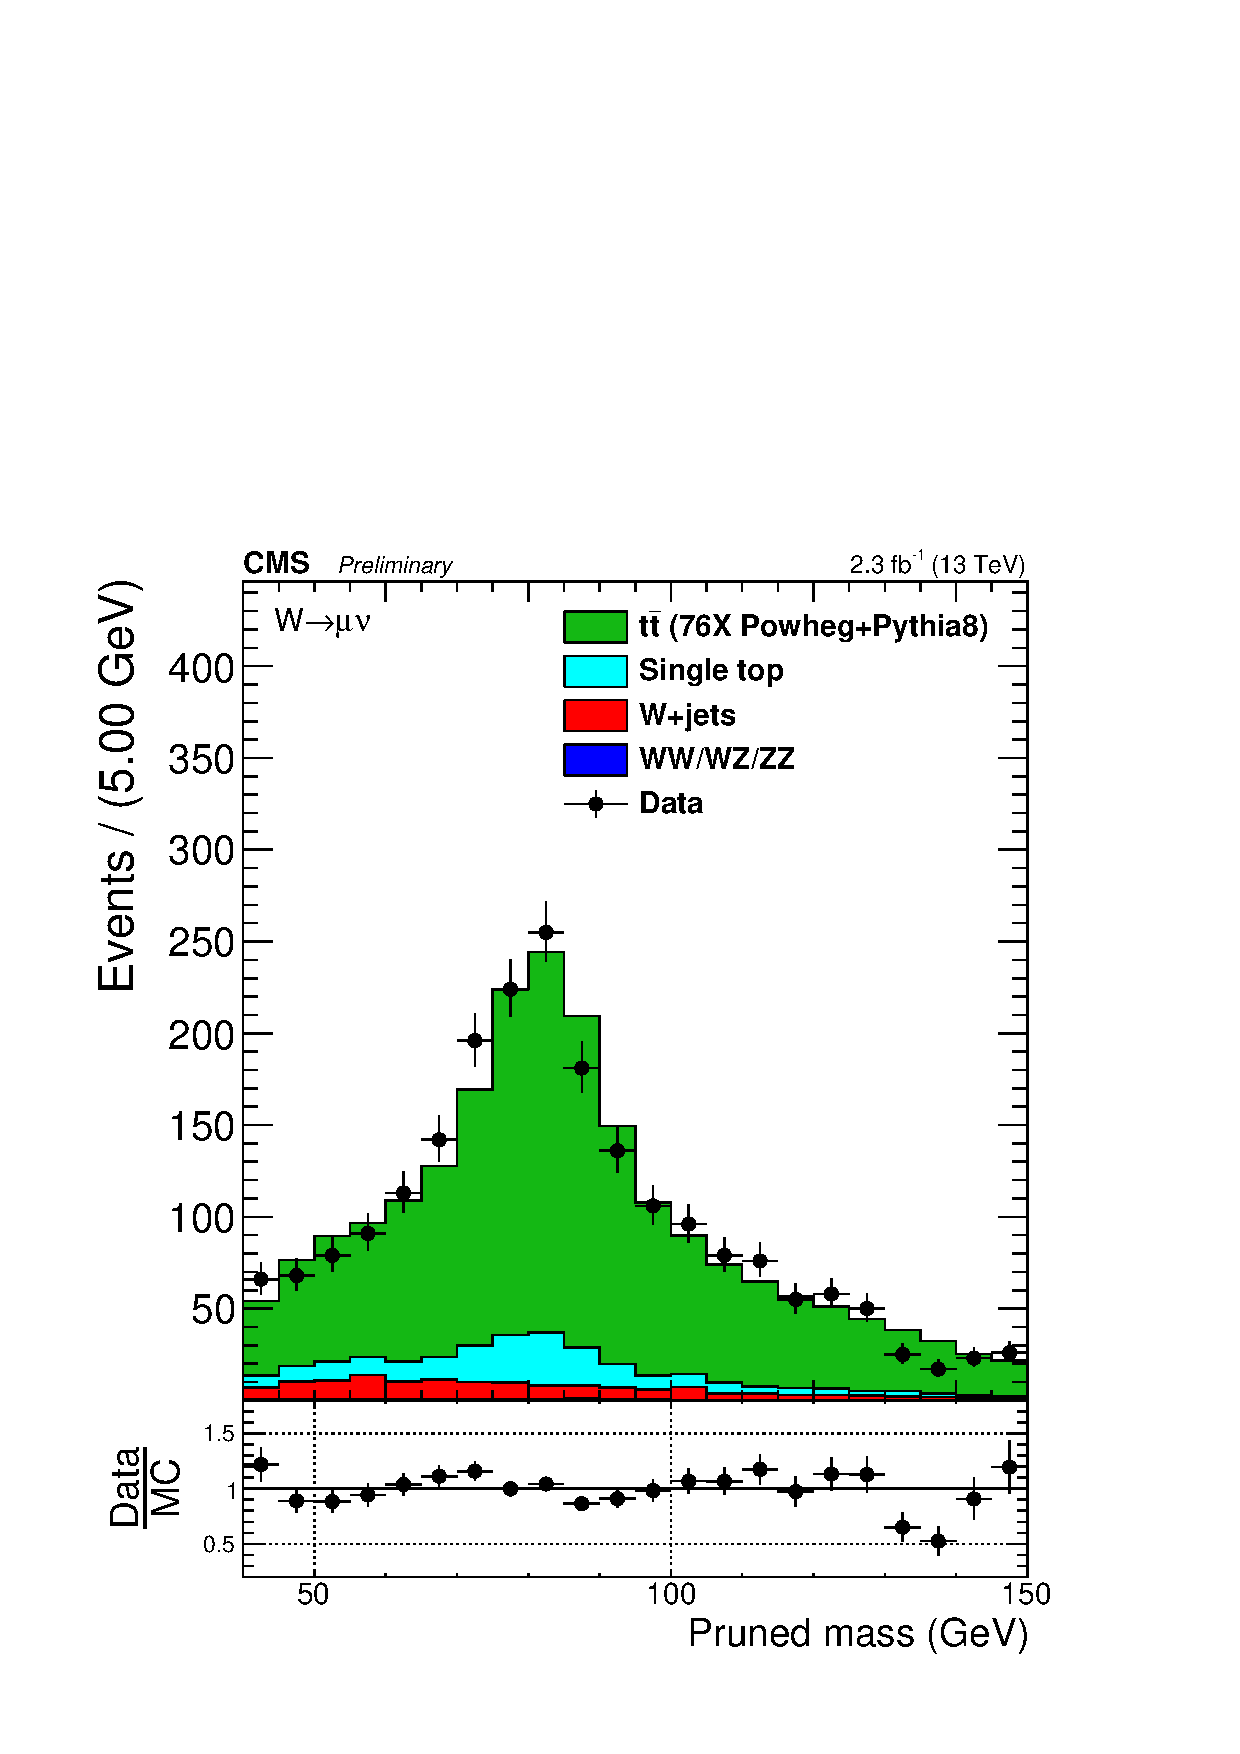
\includegraphics[width=0.4\textwidth]{figures/vtagging/AN-16-215/Whadr_pruned_mu.pdf}
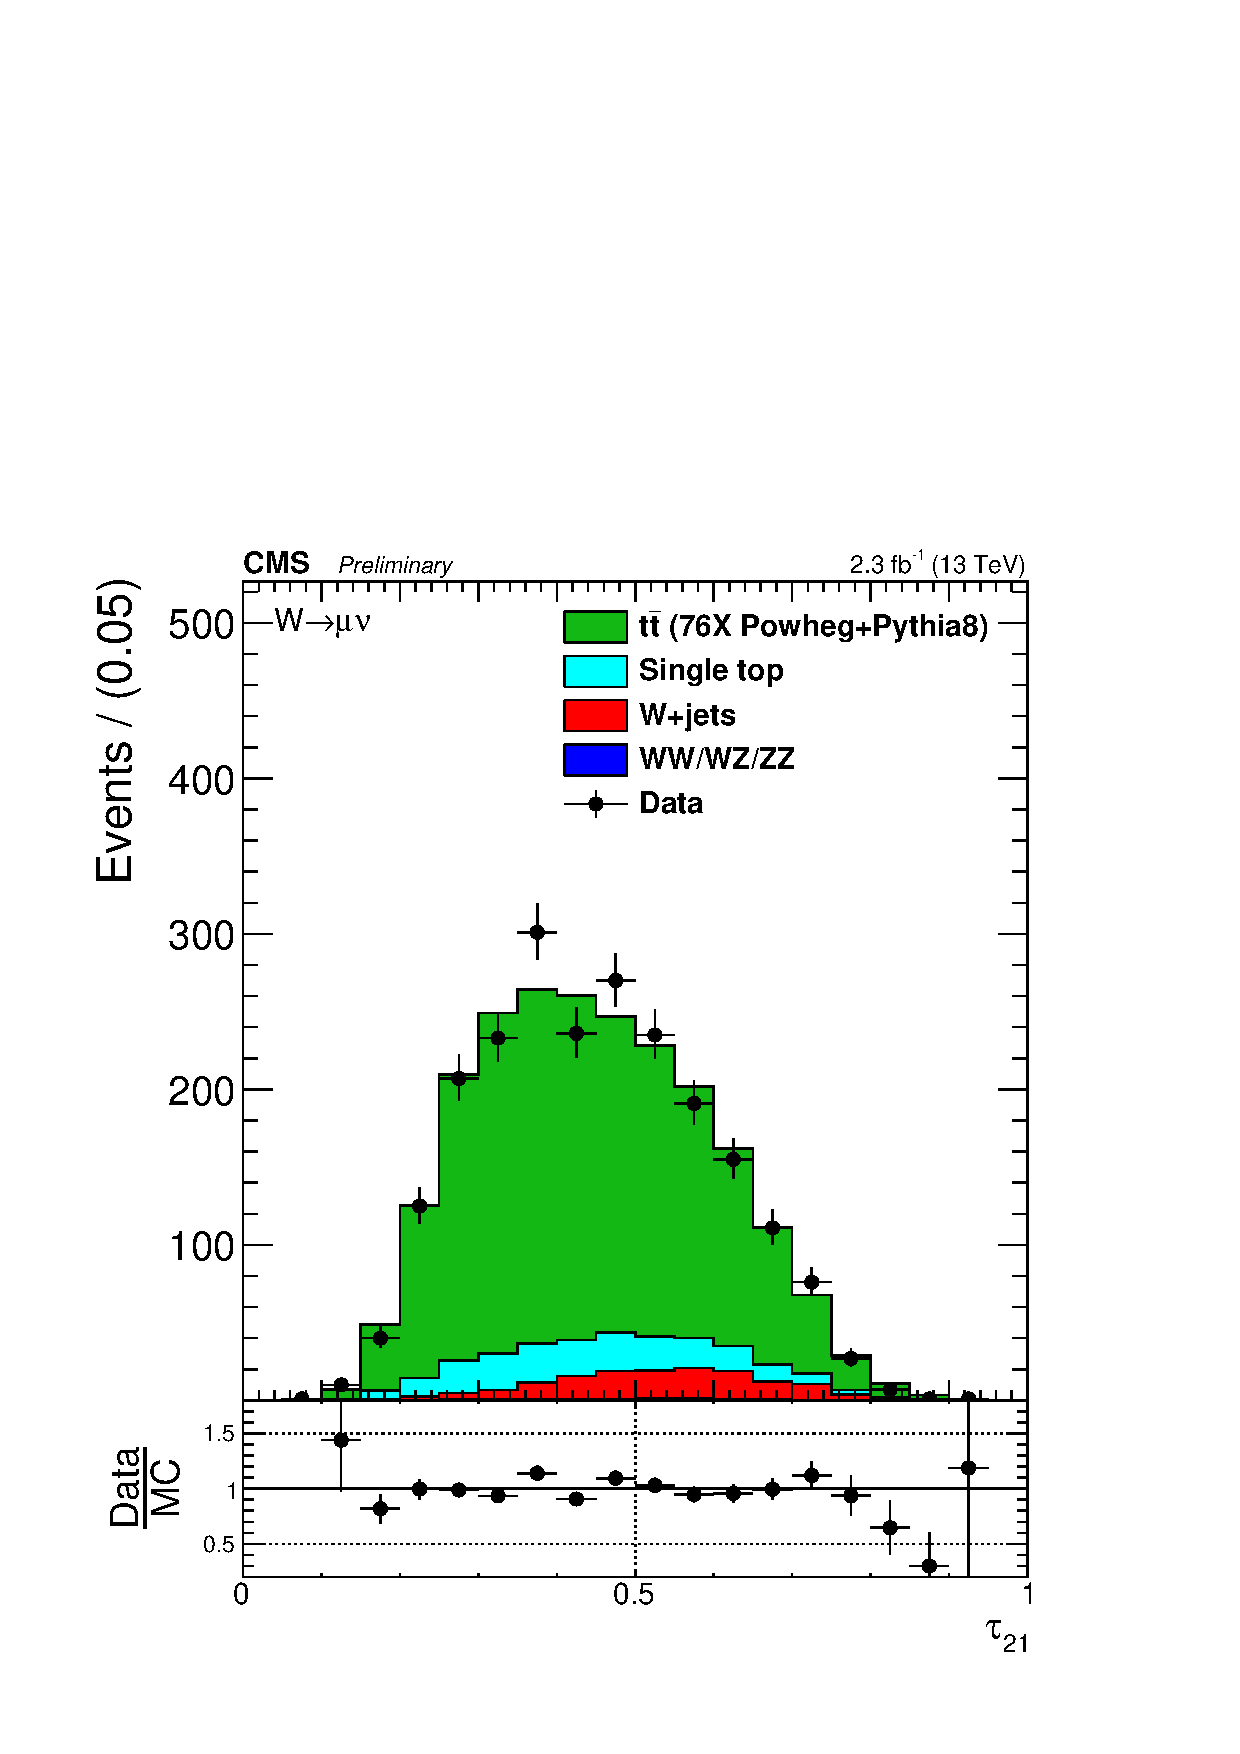
\includegraphics[width=0.4\textwidth]{figures/vtagging/AN-16-215/Whadr_tau21_mu.pdf}\\
% \includegraphics[width=0.5\textwidth]{figures/vtagging/AN-16-215/Whadr_puppi_softdrop_mu.pdf}
% \includegraphics[width=0.5\textwidth]{figures/vtagging/AN-16-215/Whadr_puppi_tau2tau1_mu.pdf}\\
\end{tabular}
\caption{Distribution of pruned jet mass (left) and n-subjettiness (right) in the \ttbar control sample.} 
\label{fig:searchI:ttbarcp}
\end{figure}
\clearpage
\subsection{Fitting procedure}
For this measurement, what we are interested in is to extract and compare the W-tagging efficiency of the combined selection of jet mass and \nsubj in data and MC. We are additionally interested in the difference in jet-mass scale (mean of the W-jet mass peak) and jet-mass resolution (width of the W-jet mass peak), as this also affects the shape of the signal jet mass and therefore the tagging efficiency. In order to study these variables, we look at the pruned jet mass spectrum between 40 and 150 \GeV in two regions: 
\begin{itemize}
\itemsep0em 
  \item Pass region: $0 <  \nsubj \leq 0.45 \sim$ high purity , and
  \item Fail region: $0.45 < \nsubj \leq 0.75\sim$ low purity.
\end{itemize}
Our goal is to understand what the real fraction of merged W jets is in the pass category and in the fail category, assuming that the sum of the two correspond to a 100\% selection efficiency (the amount of W boson jets falling outside of this region is negligible).
The strategy is as follows: We first derive probability density functions (PDFs) which describe the distribution of fully merged W boson jets and non-W boson jets in \ttbar, both in the pass and in the fail region. The PDFs describing real W jets and non-W jets are added with a fraction which is left floating: the fit decides what the fraction of real W to non-W jets is in the pass and in the fail region. A simultaneous fit of pass and fail regions is then performed (using the two composite PDFs), where the fraction of real W jets in both pass and fail regions is constrained such that, if the signal efficiency in the pass region is $\epsilon_S$, the signal efficiency in the fail region is ($1-\epsilon_S$). This is done by letting the normalization of the PDF describing real W jets in the pass category be defined as the total real W boson yield in the pass and fail regions combined, multiplied by some fraction, $\epsilon_S$. The normalization of the PDF describing real W boson jets in the fail category is then the total real W boson yield in the pass and fail regions combined, multiplied by ($1-\epsilon_S$).\par
To understand which part of the \ttbar jet mass distribution contains real, merged W boson jets and which are only pure combinatorial background, non-W jets, we start from \ttbar MC.
By matching the AK8 jet with quarks coming from the hadronic W boson at generator level, in a cone of $\Delta R < 0.8$, we can access the real merged W and non-merged W softdrop mass shapes.
The real W and non-W PDFs for jets that pass and fail the N-subjettiness selection $\nsubj < 0.45$, are found to be well described by the following functions:
\begin{align*} 
f_{\rm bkg}(m_{j}) &= F_{\textrm{ExpErf}} = e^{c_0m_{j}} \cdot \frac{1 + {\rm Erf}((m_{j}-a)/b)}{2}  &\sim\textrm{for non-\PW jets in both pass and fail }\\
f^{\rm sig}(m_{j}) &= F_{\rm Gaus}(m_{j}) + F_{\rm ExpErf}(m_{j})                                    &\sim\textrm{for real \PW jets in both pass and fail}
\end{align*}
Figure~\ref{fig:searchI:ttfitpruned} shows the fitted pruned jet mass spectrum for real W jets (upper) and non-W jets (lower) in \ttbar for jets that passed (left column) and failed (right column) the N-subjettiness selection $\tau_{21}<0.45$.

\begin{figure}[h!]
  \centering \includegraphics[width=0.3\textwidth]{figures/vtagging/AN-16-215/plots_76X/fits_TTMC/plots_em_HP0v45powheg_76X_MCfits/{_TTbar_realWExoDiBosonAnalysis.WWTree_TTbar_powheg_76X_GausErfExp_ttbar_with_pull}.pdf} \includegraphics[width=0.3\textwidth]{figures/vtagging/AN-16-215/plots_76X/fits_TTMC/plots_em_HP0v45powheg_76X_MCfits/{_TTbar_realW_failtau2tau1cutExoDiBosonAnalysis.WWTree_TTbar_powheg_76X_GausErfExp_ttbar_failtau2tau1cut_with_pull}.pdf}\\ \includegraphics[width=0.3\textwidth]{figures/vtagging/AN-16-215/plots_76X/fits_TTMC/plots_em_HP0v45powheg_76X_MCfits/{_TTbar_fakeWExoDiBosonAnalysis.WWTree_TTbar_powheg_76X_ErfExp_ttbar_with_pull}.pdf} \includegraphics[width=0.3\textwidth]{figures/vtagging/AN-16-215/plots_76X/fits_TTMC/plots_em_HP0v45powheg_76X_MCfits/{_TTbar_fakeW_failtau2tau1cutExoDiBosonAnalysis.WWTree_TTbar_powheg_76X_ErfExp_ttbar_failtau2tau1cut_with_pull}.pdf}
    \caption{Fit to the real W (upper) and non-W (lower) boson pruned jet mass distribution for jets that pass (left) and fail (right) the cut on $\tau_{21}~<$~0.45.}
  \label{fig:searchI:ttfitpruned}
\end{figure}
These shapes constitute the fit functions used for the simultaneous fit. As can be seen from the fit to real W jets in the pass region, the distribution is not purely Gaussian and has a tail at higher groomed masses. This tail depends on the matching requirements used to define real merged W jets and is unphysical. We therefore assume that the distribution of real W jets can be described by a Gaussian only, allowing the exponential error function  used to describe non W-jets to cover the contribution from the tails, thereby taking the number of real W jets as the integral of the Gaussian shape only. This eliminates two additional fit functions, corresponding to six free parameters from the fit.  In older estimations of the W-tagging scale factor based on the same procedure~\cite{CMS-PAS-B2G-16-021}), the functions used to describe the tail of the real W-jet distributions were also taken into account as contributing to the real W-jet tagging efficiency. These two calculations test two extremes: the new method assumes a Gaussian peak, absorbing the tails into the background function making the fit more robust, while the old method assumes a Gaussian peak with tails estimated from matched MC. The latter uses a more precise definition of real W jets, but yields a less robust fit. Both methods were investigated and we found that the absorption of tails into the background function resulted in a decrease in the relative uncertainty on the final scale factor of 50\% and an overall improvement on the fit quality, reducing the fit $\chi^2$ by 15\%. The fit parameters of the functions used to describe non-W jets in both the pass and in the fail region are further constrained using the values obtained from matched \ttbar MC. The W-tagging scale factors ($SF_{HP}$) for the high purity selection ($\nsubj<0.45$) are then extracted by estimating the selection efficiency ($\epsilon_{HP}$) for both data and simulated samples by fitting, simultaneously, the pass and fail categories:
\begin{align*}
\footnotesize
    L_{\rm pass} &= \prod_{i}^{N_{\rm evt}^{pass}} \bigg[N_{\rm W}\cdot\epsilon_{HP}\cdot f_{\rm pass}^{\rm sig}(m_{j}) + N_{\rm 2}\cdot f_{\rm pass}^{\rm bkg}(m_{j})+ \sum_{j=\textrm{ST,VV,WJet}} N^{j}_{\rm pass}\cdot f_{\rm pass}^{j}\bigg],\\
    L_{\rm fail} &= \prod_{i}^{N_{\rm evt}^{fail}} \bigg[N_{\rm W}\cdot(1-\epsilon_{HP})\cdot f^{\rm sig}_{\rm fail}(m_{j}) + N_{\rm 3}\cdot f_{\rm fail}^{\rm bkg}(m_{j})+ \sum_{j=\textrm{ST,VV,WJet}} N^{j}_{\rm fail}\cdot f_{\rm fail}^{j}\bigg],
\end{align*}
where $N_{W}$ is the number of real W boson jets, $N_{2}$ and $N_{3}$ are the number of combinatorial background events passing and failing the \nsubj selection, respectively, and $N_{j}$ and $f_{j}$, with $j$ = ST, VV, WJet, are the normalizations and shapes of the minor backgrounds (single top, VV, W+jets), which are fixed from simulation. The fit functions used are:
\begin{alignat*}{3}
    f_{\rm pass}^{\rm sTop} &= F_{\rm ErfExpGaus}(x) = &&\frac{1 + {\rm Erf}((x-a)/b)}{2} \cdot e^{-(x-x_{0})^{2}/2\sigma^{2}}\\
    f_{\rm fail}^{\rm sTop} &= F_{\rm ExpGaus}(x)    = &&e^{ax} \cdot e^{-(x-b)^{2}/2s^{2}},\\
    f_{\rm pass}^{\rm VV}   &= F_{\rm ExpGaus}(x)    = &&e^{ax} \cdot e^{-(x-b)^{2}/2s^{2}},\\
    f_{\rm fail}^{\rm VV}   &= F_{\rm ExpGaus}(x)    = &&e^{ax} \cdot e^{-(x-b)^{2}/2s^{2}},\\
    f_{\rm pass}^{\rm wjet} &= F_{\rm ErfExp}(x)     = &&e^{c_0x} \cdot \frac{1 + {\rm Erf}((x-a)/b)}{2},\\
    f_{\rm fail}^{\rm wjet} &= F_{\rm ErfExp}(x)     = &&e^{c_0x} \cdot \frac{1 + {\rm Erf}((x-a)/b)}{2},
\end{alignat*}
with the corresponding distributions shown in Figure~\ref{fig:searchII:minorbkr}.
\begin{figure}[h!]
   \centering \includegraphics[width=0.30\textwidth]{figures/vtagging/AN-16-215/plots_76X/plots_0v45/plots_em_HP0v45powheg_76X_MCfits/{_STopExoDiBosonAnalysis.WWTree_STop_76X_ErfExpGaus_sp}.pdf} \includegraphics[width=0.30\textwidth]{figures/vtagging/AN-16-215/plots_76X/plots_0v45/plots_em_HP0v45powheg_76X_MCfits/{_WJets0ExoDiBosonAnalysis.WWTree_WJets_76X_ErfExp}.pdf} \includegraphics[width=0.30\textwidth]{figures/vtagging/AN-16-215/plots_76X/plots_0v45/plots_em_HP0v45powheg_76X_MCfits/{_VVExoDiBosonAnalysis.WWTree_VV_76X_ExpGaus}.pdf}\\ \includegraphics[width=0.30\textwidth]{figures/vtagging/AN-16-215/plots_76X/plots_0v45/plots_em_HP0v45powheg_76X_MCfits/{_STop_failtau2tau1cutExoDiBosonAnalysis.WWTree_STop_76X_ExpGaus}.pdf} \includegraphics[width=0.30\textwidth]{figures/vtagging/AN-16-215/plots_76X/plots_0v45/plots_em_HP0v45powheg_76X_MCfits/{_WJets0_failtau2tau1cutExoDiBosonAnalysis.WWTree_WJets_76X_ErfExp}.pdf} \includegraphics[width=0.30\textwidth]{figures/vtagging/AN-16-215/plots_76X/plots_0v45/plots_em_HP0v45powheg_76X_MCfits/{_VV_failtau2tau1cutExoDiBosonAnalysis.WWTree_VV_76X_ExpGaus}.pdf}
  \caption{Fits to the pruned jet mass spectrum for the non-dominant backgrounds (Single top, W+jets and VV respectively) in the pass (upper) and fail (lower) regions.}
  \label{fig:searchII:minorbkr}
\end{figure} 
The floating parameters of the fit (besides the PDF shape parameters themselves) are the rates $N_{W}$, $N_{2}$ and $N_{3}$, and the mean and sigma of the W-mass distribution defined in
$f^{\rm sig}_{\rm pass}(m_{j})$ and $f^{\rm sig}_{\rm fail}(m_{j})$. The ratio between data and simulation efficiencies is then taken as the W-tagging scale factor:
\begin{equation}
  \label{SF}
  SF_{HP}= \frac{\epsilon_{HP}(\textrm{data})}{\epsilon_{HP}(\textrm{sim})}.
\end{equation}
Considering that, both for data and simulation, $\epsilon_{HP}+\epsilon_{LP}+\epsilon_{fail} = 1$, the scale factor for low purity category can be defined as:
\begin{equation*}
  SF_{LP} = \frac{1-\epsilon_{HP}(\textrm{data})-\epsilon_{fail}(\textrm{data})}{1-\epsilon_{HP}(\textrm{sim})-\epsilon_{fail}(\textrm{sim})},
\end{equation*}
where $\epsilon_{fail}$ is the ratio between the number of events with $\tau_2/\tau_1 > 0.75$ and the total number of events. As mentioned previously, the number of real \PW jets with $\tau_2/\tau_1 > 0.75$  is negligible and the definition of the low purity scale factor simplifies to
\begin{equation}
  SF_{LP} = \frac{1-\epsilon_{HP}(\textrm{data})}{1-\epsilon_{HP}(\textrm{sim})}.
\end{equation}

\subsection{Systematic uncertainties}
\label{sec:searchI:wtagsystematic}
As systematic uncertainties, we consider effects due to differences between \ttbar simulation as well as effects due to the choice of fit method. The former is evaluated by comparing the extracted scale factor when using \ttbar MC samples produced with three different combinations of matrix element (ME) and shower generators: \POWHEG (NLO) interfaced with \PYTHIA{8} , \MADGRAPH (LO) QCD interfaced with \HERWIG{++}, and \POWHEG interfaced with \HERWIG{++}. The uncertainty due to different ME generators (\POWHEG versus \MADGRAPH) corresponds to 3(13)\% and is listed in Table~\ref{tab:searchI:WtagSFs} as the first quoted systematic uncertainty. The uncertainty due to parton showering (\PYTHIA{8} versus \HERWIG{++}) is 8.6\%, but is not relevant for analyses where no \HERWIG{++} based simulation is used, as is the case for the search presented in this chapter. 
For the systematic uncertainty accounting for effects due to choice of fit method, we compare the estimated extracted efficiency in \ttbar MC using the two different fit models described above: the new model, where the signal is modeled by a Gaussian peak and the tails of the distribution are absorbed in the background fit model, and the old model, including the tails when calculating the fraction of real W jets. Figure~\ref{fig:searchII:gausvstails} shows the fits obtained in the pass and fail regions using the two different models. With the new model only the Gaussian component of the fit contributes to the W-tagging efficiency while, with the old model, a Chebyshev component is additionally contributing to the total W-tagging efficiency.
\begin{figure}[h!]
  \centering
    \includegraphics[width=0.33\textwidth]{figures/vtagging/AN-16-215/2Gauss.pdf}
    \includegraphics[width=0.33\textwidth]{figures/vtagging/AN-16-215/GausErfExpPass.pdf}\\
    \includegraphics[width=0.33\textwidth]{figures/vtagging/AN-16-215/GausChebysgev.pdf}
    \includegraphics[width=0.33\textwidth]{figures/vtagging/AN-16-215/GausErfExpFail.pdf}
  \caption{Fits obtained in the pass (top) and fail (bottom) regions using two different models: An alternative model with tails (top and bottom, left) where the tail component is contributing to the total W-tagging efficiency. When using the default model (top and bottom, right), only the Gaussian component of the fit contributes to the W-tagging efficiency.}
  \label{fig:searchII:gausvstails}
\end{figure} 
The estimated efficiencies obtained using both methods, after being corrected for the fraction of W jets in the tails, agree within 0.3(0.8)\% and are listed as a systematic uncertainty in Table~\ref{tab:searchI:WtagSFs}.\par
One additional uncertainty is added. As the W-tagging scale factor is evaluated in a \ttbar sample, the transverse momentum range is rather limited. When the W-jet \PT reaches $\sim 400 \GeV$, the AK8 jet becomes a fully merged top jet with a mass of 170 \GeV and a scale factor measurement becomes impossible. However, the jets used in the analyses presented in this thesis have very high transverse momenta, up to 2-3 \TeV, and we therefore need an estimate of how the uncertainty on the W-tagging scale factor changes as a function of \PT. This is estimated by comparing the difference in tagging efficiency between $\BulkG \rightarrow \PW \PW$ signal MC showered by \PYTHIA{8} as compared to \HERWIG{++} as a function of jet \PT, relative to the difference in tagging efficiency between the two at a $\PT \sim 200$~\GeV. This measurement was performed by a separate analysis team, and found to be $5.90\% \times \ln(\pt/200\GeV)$.
% \begin{figure}[h!]
%   \centering
%     \includegraphics[width=0.50\textwidth]{figures/vtagging/AN-16-215/wtag-ptdependence-tau21tight.pdf}
%   \caption{Uncertainty on the \pt dependence of the scale factor as a function of \pt, approximated with a logarithmic function.}
%   \label{fig:ptdependence}
% \end{figure}
Systematic uncertainties from other sources (lepton identification, b tagging, etc.) are less than 0.5\% and therefore negligible.

\subsection{Fit results}
The simultaneous fit as described above is then performed both for data and for simulation, where we take the ratio of data and MC efficiencies as efficiency scale factors. The corresponding fits are shown in Figure~\ref{fig:searchII:simfit}, with the corresponding extracted efficiencies and scale factors summarized in Table~\ref{tab:searchI:WtagSFs}.
\begin{table}[h!]
   \centering
   \footnotesize
   \begin{tabular}{ l | c | c | c | c }
    & Working point & Eff. data & Eff. simulation & Scale factor\\
   \hline
   HP&$\nsubj < 0.45$& $0.775 \pm 0.041 $& $0.822 \pm 0.033$ &$0.94 \pm 0.05~\rm{(stat)} \pm 0.03~\rm{(sys)} \pm 0.003~\rm{(sys)}$\\
   LP&$0.45 < \nsubj < 0.75$& $0.225 \pm 0.041 $& $0.178 \pm 0.033$ &$1.27 \pm 0.25~\rm{(stat)} \pm 0.13~\rm{(sys)} \pm 0.008~\rm{(sys)}$\\
   \hline
   \end{tabular}
   \caption{Efficiencies in data and in MC together with the corresponding W-tagging scale factors for the high purity and low purity categories. }
   \label{tab:searchI:WtagSFs}
\end{table}
\begin{figure}[h!]
\centering
\includegraphics[width=0.44\textwidth]{figures/vtagging/AN-16-215/_HP0v45powheg_76X_em_pTbin_200_5000.pdf}
\includegraphics[width=0.44\textwidth]{figures/vtagging/AN-16-215/_HP0v45powheg_76X_em_fail_pTbin_200_5000.pdf} \\
\caption{Pruned jet mass distribution that pass (left) and fail (right) the $\nsubj < 0.45$ selection. Results of both the fit to data (blue) and simulation(red) are shown. The background components of the fit are shown as short-dashed lines.}
\label{fig:searchII:simfit}
\end{figure}
\noindent We additionally extract the jet mass scale and jet mass resolution, used to scale and smear the jet mass signal shape in the limit setting procedure. These values are taken from the mean $\langle m \rangle$ and width $\sigma$ of the Gaussian
component of the simultaneous fit in the pass region and are summarized in Table~\ref{tab:searchI:params}. Both the jet mass scale as well as the jet mass resolution is larger in simulation than in data with a relative difference of 2 and 10\%, respectively.
However, the jet mass resolution scale factor has a large uncertainty attached to it and is statistically insignificant (in agreement with unity within uncertainty).
\begin{table}[!h]
 \begin{center}
 \begin{tabular}{l|c|c|c}
  Parameter & Data & Simulation & Data/Simulation \\
  \hline
  Pruning $\langle m \rangle$ &$80.9 \pm 0.6~{\rm \GeV}$   & $82.5 \pm 0.1~{\rm \GeV}$  & $0.980 \pm 0.007$ \\
  Pruning $\sigma$            & \ $6.7 \pm 0.7~{\rm \GeV}$ & \ $7.5 \pm 0.3~{\rm \GeV}$ & $0.89 \pm 0.10$ \\
  \hline
  % PUPPI softdrop $\langle m \rangle$ &$86.8 \pm 0.8~{\rm \GeV}$ & $87.9 \pm 0.2~{\rm \GeV}$ & $0.988 \pm 0.010$ \\
%   PUPPI softdrop $\sigma$ & \ $9.2 \pm 1.0~{\rm \GeV}$ & \ $8.7 \pm 0.4~{\rm \GeV}$ & $1.07 \pm 0.09$ \\
  % PUPPI softdrop $\langle m \rangle$ &$80.3 \pm 0.8~{\rm \GeV}$ & $81.9 \pm 0.01~{\rm \GeV}$ & $0.98 \pm 0.01$ \\%New mass corrections
  % PUPPI softdrop $\sigma$ & \ $9.0 \pm 0.9~{\rm \GeV}$ & \ $8.5 \pm 0.4~{\rm \GeV}$ & $1.07 \pm 0.12$ \\%New mass corrections
 \end{tabular}
 \caption{Jet mass scale and resolution in data and in simulation together with the relevant data-simulation scale factors.}
 \label{tab:searchI:params}
 \end{center}
\end{table}

\subsection{Impact on search variables}
\label{sec:searchI:wtagimpact}
The obtained W-tagging scale factors are used as a scale of the signal yield. As we require two W-tagged jets, either HP or LP, the actual scale factors for the high-purity signal yield is $\textrm{SF}_{HP}\times\textrm{SF}_{HP}$ and for the low-purity category $\textrm{SF}_{HP}\times\textrm{SF}_{LP}$. The signal yields are then
\begin{align*}
N_{S}^{HP} &= N_{\textrm{HP tot. yield}} \times \textrm{SF}_{HP} \times \textrm{SF}_{HP}\\
N_{S}^{LP} &= N_{\textrm{LP tot. yield}} \times \textrm{SF}_{HP} \times \textrm{SF}_{LP}\\
\end{align*}
The uncertainties on the scale factors are considered as anti-correlated between the HP and the LP categories.
The jet mass scale and resolution are used to scale and smear the signal Monte Carlo. An uncertainty on the signal yield based on the uncertainty on jet mass scale and resolution is also considered by scaling and smearing the jet mass up and down within the quoted uncertainties and then recomputing the signal efficiency. The results are listed in Table~\ref{tab:searchI:sys}.
% With a HP relative uncertainty of 6\% and LP relative uncertainty of 22\%, this becomes
% \begin{align*}
% \sigma_{rel}^{HPHP} &= 1.06 \times 1.06 = 1.12\\
% \sigma_{rel}^{HPLP} &= 1.28 \times 1.06 = 1.36\\
% \end{align*}
  
\section{Systematic uncertainties}
\label{sec:searchI:sys}
The uncertainty on the background parametrization is statistical only and is taken as the covariance matrix of the dijet fit function. As demonstrated in the F-test, we study different background parameterizations and we have found these to be within the fit uncertainty of the nominal fit. The remaining uncertainties concern the signal shape and yield and are listed in Table~\ref{tab:searchI:sys}. Jet reconstruction uncertainties affect both the signal yield and the signal shape. These are evaluated by rescaling the jet four-momenta according to uncertainties on the jet energy scale and resolution and recomputing the signal efficiency. The difference in efficiency with and without smearing/scaling is taken as a systematic uncertainty, as described above.
The jet mass/energy scale and resolution also affect the signal shape, and are added as uncertainties in the peak position and width of the Gaussian component of the signal PDFs.
\begin{table}[h!]
  \footnotesize
  \centering
  \begin{tabular}{lccc}
    \hline
    Source                           & Relevant quantity    & HP uncertainty (\%)  & LP uncertainty (\%)\\
    \hline
    Jet energy scale                 & Resonance shape      & 2                    & 2 \\
    Jet energy resolution            & Resonance shape      & 10                   & 10 \\
    \hline
    Jet energy and \mJ{} scale       & Signal yield         & \multicolumn{2}{c}{0.1--4}\\ 
    Jet energy and \mJ{} resolution  & Signal yield         & \multicolumn{2}{c}{0.1--1.4}\\
    Pileup                           & Signal yield         & \multicolumn{2}{c}{2}\\
    Integrated luminosity            & Signal yield         & \multicolumn{2}{c}{2}\\
    PDFs (\PWpr)                     & Signal yield		      & \multicolumn{2}{c}{4--19}\\
    PDFs (\PZpr)                     & Signal yield		      & \multicolumn{2}{c}{4--13}\\
    PDFs (\BulkG)                    & Signal yield		      & \multicolumn{2}{c}{9--77}\\
    Scales (\PWpr)                   & Signal yield		      & \multicolumn{2}{c}{1--14}\\
    Scales (\PZpr)                   & Signal yield		      & \multicolumn{2}{c}{1--13}\\
    Scales (\BulkG)                  & Signal yield		      & \multicolumn{2}{c}{8--22}\\
    \hline
    Jet energy and \mJ{} scale       & Migration            & \multicolumn{2}{c}{1--50}\\
    V tagging \nsubj{}               & Migration            & 14                    & 21\\
    V tagging \pt-dependence         & Migration            & 7--14                & 5--11\\
    \hline
  \end{tabular}
  \caption{Summary of the systematic uncertainties and the quantities they affect. Migration uncertainties result in events switching between the purity/mass categories and change the efficiency in each category, but do not affect the total signal efficiency.}
  \label{tab:searchI:sys}
\end{table}


\clearpage

\section{Results}
\label{sec:searchI:results}
The background fits for each analysis category in the data signal region are shown in Figure \ref{fig:search1:bkgfitMassCat}. Here a background-only fit is performed while, as described above, a simultaneous fit is used for the limit-setting procedure. The filled area corresponds to the $1 \sigma$ error band of the background fit, obtained using linear error propagation.
\begin{figure}[h!]
\centering
\includegraphics[width=0.45\textwidth]{figures/analysis/search1/AN-15-211/fits/MLfits/BkgFit_DijetMassHighPuriWW.pdf}
\includegraphics[width=0.45\textwidth]{figures/analysis/search1/AN-15-211/fits/MLfits/BkgFit_DijetMassLowPuriWW.pdf}\\
\includegraphics[width=0.45\textwidth]{figures/analysis/search1/AN-15-211/fits/MLfits/BkgFit_DijetMassHighPuriWZ.pdf}
\includegraphics[width=0.45\textwidth]{figures/analysis/search1/AN-15-211/fits/MLfits/BkgFit_DijetMassLowPuriWZ.pdf}\\
\includegraphics[width=0.45\textwidth]{figures/analysis/search1/AN-15-211/fits/MLfits/BkgFit_DijetMassHighPuriZZ.pdf}
\includegraphics[width=0.45\textwidth]{figures/analysis/search1/AN-15-211/fits/MLfits/BkgFit_DijetMassLowPuriZZ.pdf}
\caption{Fit to data in the signal region using the background fit only for the different mass and purity categories. The filled red area correspond to the $1 \sigma$  statistical error of the fit.}
\label{fig:search1:bkgfitMassCat}
\end{figure}
No excess is observed, and we proceed by setting upper limits on the cross section times branching ratio of the process $\text{X} \to \VV$, using the asymptotic $\textrm{CL}_\textrm{S}$ method~\cite{CLs}. The binned likelihood is defined as
\begin{equation}
L = \prod_i\frac{\mu^{n_i}_ie^{-\mu_i}}{n_i!},
\end{equation}
with
\begin{equation}
\mu_i=\sigma \cdot N_i(S)+N_i(B).
\end{equation}
Here $\sigma$ is the signal strength scaling the expected number of signal events in the $i$-th dijet invariant-mass bin $N_i(S)$, $N_i(B)$ is the expected number of background events in dijet invariant-mass bin $i$ and $n_i$ is the observed number of events in the $ith$ dijet invariant-mass bin. The background per bin $N_i(B)$ is estimated from the background component of the best signal and background fit to the data points, with the signal cross section set to zero. The number of signal events in the $i$-th dijet invariant mass bin, $N_i(S)$, is estimated from the signal templates, considering only dijet invariant massed in a 20\% window around the resonance mass, containing most of the signal contribution while making sure to keep a good description of the core.

\section{Limits}
\subsection{All-hadronic analysis only}
\label{sec:searchI:results4q}
As mentioned in Section~\ref{sec:searchI:samples}, we set limits on three different signal scenarios: $\BulkG \rightarrow \WW$, $\BulkG \rightarrow \ZZ$, and $\PWpr \rightarrow WZ$, with a $\ktilde = 0.5$ for the \BulkG. Figure \ref{fig:searchI:Limits_CombNew} shows the asymptotic limits at 95 \% confidence level on the signal cross section as a function of its resonance mass obtained with 2.7 \fbinv of 13 \TeV CMS data after combining all mass and purity categories (top). The corresponding p-values are shown in the bottom panel.
\begin{figure}[h!]
\centering
\includegraphics[width=0.32\textwidth]{figures/analysis/search1/AN-15-211/limits/brazilianFlag_BulkWW_new_combined_13TeV.pdf}
\includegraphics[width=0.32\textwidth]{figures/analysis/search1/AN-15-211/limits/brazilianFlag_WZ_new_combined_13TeV.pdf}
\includegraphics[width=0.32\textwidth]{figures/analysis/search1/AN-15-211/limits/brazilianFlag_BulkZZ_new_combined_13TeV.pdf}\\
\includegraphics[width=0.32\textwidth]{figures/analysis/search1/AN-15-211/pvalues/pvalue_BulkWWin_combined_new.pdf}
\includegraphics[width=0.32\textwidth]{figures/analysis/search1/AN-15-211/pvalues/pvalue_WZin_combined_new.pdf}
\includegraphics[width=0.32\textwidth]{figures/analysis/search1/AN-15-211/pvalues/pvalue_BulkZZin_combined_new.pdf}\\
\caption{Expected and observed limits with corresponding p-values obtained using 2.7 \fbinv of CMS data after combining all mass and purity categories. Here for a Bulk $G\rightarrow WW$ (left), $W'\rightarrow WZ$ (middle), and $G\rightarrow ZZ$ (right) signal.}
\label{fig:searchI:Limits_CombNew}
\end{figure}
The statistics are too low to exclude the excess around 2 \TeV observed in the corresponding Run 1 analysis and, in addition, an under-fluctuation in data is present in this region. The largest excess of 2.8 $\sigma$ is observed for a $\BulkG \rightarrow \ZZ$ hypothesis at a resonance mass of 2.8-3 TeV. This is driven by the high-purity ZZ mass category, the category with the lowest statistics, and is caused by one event. A 3-parameter fit is the default background fit function for this category, however, a 2-parameter fit could also be used to describe these data. In Figure \ref{fig:searchI:Limits_ZZHP} we compare the limits and p-values obtained using a 2-parameter and a 3-parameter fit to describe the background in this category. The significance at 3 TeV is reduced from 2.8 to 1.5 $\sigma$ with a 2-parameter fit, reflecting the fact that the fit is poorly constrained in the high mass tail due to low statistics. The fit to data using both a 2 and 3-parameter fit in the ZZ high-purity category is shown in Figure~\ref{fig:app:ZZHP2vs3p}, where we see that the 2-parameter fit lies within the fit uncertainties of the nominal fit.
\begin{figure}[h!]
\centering
\includegraphics[width=0.45\textwidth]{figures/analysis/search1/AN-15-211/limits/brazilianFlag_BulkZZ_ZZHP_13TeV.pdf}
\includegraphics[width=0.45\textwidth]{figures/analysis/search1/AN-15-211/limits/brazilianFlag_BulkZZ_ZZHP_2parFit__13TeV.pdf}\\
\includegraphics[width=0.45\textwidth]{figures/analysis/search1/AN-15-211/pvalues/pvalue_BulkZZinZZ_high_purity.pdf}
\includegraphics[width=0.45\textwidth]{figures/analysis/search1/AN-15-211/pvalues/pvalue_BulkZZinZZ_high_purity_2par.pdf}
\caption{Expected and observed limits (top) and the corresponding p-values (bottom) obtained in the ZZ high-purity category using a 3- (left) and 2-parameter (right) fit to describe the background. The significance at 3 TeV is reduced from 2.8 to 1.5 $\sigma$.}
\label{fig:searchI:Limits_ZZHP}
\end{figure}
\begin{figure}[h!]
\centering
\includegraphics[width=0.45\textwidth]{figures/analysis/search1/misc/CMS-PAS-EXO-15-002_Figure_004-e.pdf}
\caption{Background fit to data in the ZZHP category using the nominal 3- (red) and an alternate 2-parameter (blue) fit to describe the background.}
\label{fig:app:ZZHP2vs3p}
\end{figure}
The lack of constraint on the fit in the dijet invariant mass tail when statistics are very low is a drawback of a method relying fully on a parametric fit and reduces the analysis sensitivity in the high-\mjj region. In Search II (Section~\ref{searchII}) we will keep taking advantage of the dijet fit, however, the integrated luminosity is $\sim 15$ times higher, resulting in more datapoints in the \mjj tail which further constrains the fit. In Search III (Section~\ref{searchIII}), we will explore alternate methods which allow more control over the background shape across the full mass spectrum. 

\subsection{Semi-leptonic and all-hadronic combination}
\label{sec:searchI:resultsComb}
To maximize the search sensitivity, we combine the results obtained above with those of the corresponding semi-leptonic analysis. We assume the uncertainties on luminosity, V-tagging efficiency, and jet mass scale and resolution to be fully correlated. The obtained exclusion limits in Figure~\ref{fig:searchI:limitCombined} show the resulting expected and observed exclusion limits after combining the two analyses. As before, we consider a scenario where only either a \PWpr or \PZpr resonance is expected, called the singlet hypothesis (upper two plots). In addition, we set limits on the triplet hypothesis, assuming the \PWpr and \PZpr bosons to be degenerate in mass (bottom left plot). The all-hadronic analysis sets stronger upper limits than the semi-leptonic analysis above 1.7\TeV for a \PZpr and $>$ 1.3\TeV for a \PWpr. The improvement in sensitivity is due to the higher branching fraction, such that $\cal B$($\PW\PW\to\qqbar\qqbar$) = 44\%, $\cal B$($\PW\PW\to\ell\Pgn\qqbar$) = 31\%, $\cal B$($\PW\PZ\to\qqbar\qqbar$) = 46\%, and $\cal B$($\PW\PZ\to\ell\Pgn\qqbar$) = 16\%. 
The analysis sensitivity for \BulkG is too weak to set limits, but cross sections between 3--1200\unit{fb} are excluded.
For the HVT models A and B, a \PWpr is excluded below $2.0$ and $2.2 \TeV$, respectively, and \PZpr resonances are excluded below $1.7~(1.6)\TeV$ assuming a HVT model A(B). Assuming a HVT Model A(B) triplet hypothesis, resonances below 2.3 (2.4) \TeV are excluded.
\begin{figure}[!h]
\centering
\includegraphics[width=0.49\textwidth]{figures/analysis/search1/B2G-16-004//EXOVVhvt_JJLVJZPRIME13_UL_Asymptotic_log.pdf}
\includegraphics[width=0.49\textwidth]{figures/analysis/search1/B2G-16-004//EXOVVhvt_JJLVJWPRIME13_UL_Asymptotic_log.pdf}\\     
\includegraphics[width=0.49\textwidth]{figures/analysis/search1/B2G-16-004//EXOVVhvt_JJLVJHVT13_UL_Asymptotic_log.pdf}%
\includegraphics[width=0.49\textwidth]{figures/analysis/search1/B2G-16-004//EXOVVbulkg_ALL13_UL_Asymptotic_log.pdf}
\caption{Observed (black solid) and expected (black dashed) 95\% CL upper limits on the production of a narrow-width resonance decaying to 
a pair of vector bosons for different signal hypotheses. In the upper plots, limits are set in the context of a spin-1 neutral \PZpr (left) and charged \PWpr (right) resonance, and compared with the prediction of the HVT Models A and B. In the lower left plot, limits are set in the same model under the triplet hypothesis (\PWpr and \PZpr of degenerate mass). In the lower right plot, limits are set in the context of a bulk graviton with $\ktilde =0.5$ and compared with the prediction.
}
\label{fig:searchI:limitCombined}
\end{figure}
The combined results would therefore just exclude a $\PWpr$ with a mass around 2 \TeV, the favored candidate to explain the diboson excess observed in 8 TeV data.
However, Bulk Graviton signals were still far from excluded and, with the expected increase in luminosity of a factor of ten in 2016, we were excited to keep on searching.

% Figure~\ref{fig:hvtscan} shows a scan of the coupling parameters and the corresponding observed 95\% CL exclusion
% contours in the HVT model for the combined analyses. The parameters
% are defined as $g_{\rm V}c_{\rm H}$ and $g^2c_{\rm F}/g_{\rm V}$,  related to the coupling strengths of the new resonance to
% the Higgs boson and to fermions. The range of the scan is limited by the assumption that the
% new resonance is narrow.  A contour is overlaid, representing the region where the theoretical
% width is larger than the experimental resolution of the searches, and hence where the narrow-resonance assumption is not satisfied.
% This contour is defined by a predicted resonance width of 5\%, corresponding to the narrowest resonance mass resolution of the searches.

% \begin{figure}[!htb]
% \centering
%      \includegraphics[width=0.49\textwidth]{figures/analysis/search1/B2G-16-004/hvt-couplings.pdf}
% \caption{
% Exclusion regions in the plane of the HVT couplings ($g^2c_{\rm F}/g_{\rm V},g_{\rm V}c_{\rm H}$) for three
% resonance masses, 1.5, 2.0, and 3.5\TeV. Model points A and B of the benchmarks used in the analysis are also shown.
% The solid, dashed, and dashed-dotted lines represent the boundaries of the regions excluded by this search for different resonance masses (the region outside these lines is excluded).
% The areas indicated by the solid shading correspond to
% regions where the resonance width is predicted to be more than 5\% of the resonance mass and
% the narrow-resonance assumption is not satisfied.}
% \label{fig:hvtscan}
% \end{figure}









